\documentclass[12pt,a4paper]{report}
\usepackage[a4paper,margin=1in]{geometry}
\usepackage[hidelinks]{hyperref}
\usepackage{caption}
\usepackage{graphicx}
\usepackage{subcaption}
\usepackage{lmodern}
\usepackage{setspace}
\usepackage{titlesec}
\usepackage{lipsum}
\usepackage{fancyhdr}
\usepackage{xcolor}
\usepackage{float}
\usepackage{tcolorbox}
\usepackage{amssymb}
\usepackage{amsmath}
\usepackage{algorithm}
\usepackage{algorithmic}
\usepackage{pifont}
\usepackage{booktabs}
\usepackage{colortbl}
\usepackage{tabularx} 
\usepackage{ragged2e}
\usepackage{longtable}
\usepackage[Sonny]{fncychap}
\usepackage[acronym, nonumberlist]{glossaries}
\makeglossaries




% Load acronym definitions
% acronyms.tex
\newacronym{tcr}{TCR}{T-cell receptor}
\newacronym{mmr}{MMR}{Measles, Mumps, and Rubella}
\newacronym{shap}{SHAP}{SHapley Additive exPlanations}
\newacronym{enn}{ENN}{Edited Nearest Neighbours}
\newacronym{pca}{PCA}{Principal Component Analysis}
\newacronym{wbc}{WBC}{white blood cell counts}
\newacronym{rbc}{RBC}{red blood cell counts}
\newacronym{hgb}{HGB}{hemoglobin levels}
\newacronym{hct}{HCT}{hematocrit levels}
\newacronym{plt}{PLT}{platelet counts}
\newacronym{lym}{LYM}{lymphocytes}
\newacronym{mon}{MON}{monocytes}
\newacronym{gra}{GRA}{granulocytes}
\newacronym{kknn}{kNN}{k-nearest neighbors}
\newacronym{smote}{SMOTE}{Synthetic Minority Over-sampling Technique}
\newacronym{adasyn}{ADASYN}{Adaptive Synthetic Sampling}
\newacronym{ros}{ROS}{Random Over-Sampling}
\newacronym{rna}{RNA}{Ribonucleïnezuur}

\captionsetup{font=small} 

\newcommand{\todo}[1]{%
  \par\noindent%
  \begin{tcolorbox}[colback=yellow, colframe=black, boxrule=0.5pt, sharp corners, width=\linewidth, before skip=5pt, after skip=5pt]
    \textbf{TODO:} #1
  \end{tcolorbox}%
  \par
}

\newcommand{\answer}[1]{%
  \par\noindent%
  \begin{tcolorbox}[colback=blue!10!white, colframe=blue!80!black, boxrule=0.5pt, sharp corners, width=\linewidth]
    \textbf{ANSWER:}~#1
  \end{tcolorbox}%
}

% REMARK (orange with ! icon)
\newcommand{\remark}[1]{%
  \par\noindent%
  \begin{tcolorbox}[ colback=orange!20!white, colframe=orange!80!black, boxrule=0.5pt, sharp corners, width=\linewidth, ]
    {\textbf{\textcolor{orange!80!black}!REMARK:}}~#1
  \end{tcolorbox}%
}

%--------------------------------
% Chapter Title
%--------------------------------
\ChNameVar{\raggedleft\bfseries\Large}   % "CHAPTER" word
\ChNumVar{\raggedleft\bfseries\Large}    % Chapter number
\ChTitleVar{\raggedleft\bfseries\Large}  % Chapter title

%--------------------------------
% Section Title
%--------------------------------
\titleformat{\section}[block]
    {\titlerule[2pt]\addvspace{0.8ex}%
    \bfseries\Large}
    {\thesection}{0.5em}
    {}[{\addvspace{0.4ex}\titlerule[2pt]}]
\titlespacing{\section}{0pt}{*4}{*4}

% Display current section in header:
\pagestyle{fancy}
\fancyhf{}
\fancyhead[L]{\nouppercase{\rightmark}}
\fancyfoot[C]{\thepage}

\begin{document}

% Title Page
\begin{titlepage}
    \centering
    
    % University logo at the top
    
\includegraphics[width=0.3\textwidth]{images/uantwerpen_logo.png}\\[1cm]
    {\Huge \textbf{Multimodal Data Integration for Predictive Modelling of Measles Vaccine Response with Cross-Vaccine Marker Validation}} \\
    \vfill
    
    {\Large \textbf{Elias Dams}}\\[1cm]
    
    \textbf{Promotor:} Dr. Pieter Meysman\\
    \textbf{Supervisor:} Fabio Affaticati\\[1.5cm]
    
    {\Large \textbf{University of Antwerp}}\\
    {\large Faculty of Science}\\[0.5cm]
    
    \textbf{2024-2025}\\[1.5cm]
    
    Submitted in fulfilment of the requirements for the degree of\\
    \textbf{Master in Computer Science: AI \& Data Science}\\[1cm]
    
    \textbf{June 2025}\\[2cm]
    
    % Decorative line at the bottom
    \vfill

\end{titlepage}

% Disclaimer Page
\clearpage
\thispagestyle{empty}
\vspace*{\fill}               % push content to bottom
\noindent
\begin{minipage}[b]{\textwidth}
  \raggedright
  \textbf{Disclaimer Master’s thesis}\\[2ex]
  This document is an examination document that has not been corrected for any errors identified. Without prior written permission of both the supervisor(s) and the author(s), any copying, copying, using or realizing this publication or parts thereof is prohibited. For requests for information regarding the copying and/or use and/or realisation of parts of this publication, please contact to the university at which the author is registered.\\[2ex]
  Prior written permission from the supervisor(s) is also required for the use for industrial or commercial utility of the (original) methods, products, circuits and programs described in this thesis, and for the submission of this publication for participation in scientific prizes or competitions.\\[2ex]
  This document is in accordance with the faculty regulations related to this examination document and the Code of Conduct. The text has been reviewed by the supervisor and the attendant.
\end{minipage}
\clearpage

% Table of Contents
\pagenumbering{roman}
\tableofcontents
\newpage

% List of Figures
\phantomsection
\addcontentsline{toc}{chapter}{List of Figures}
\listoffigures

% List of Tables
\phantomsection
\addcontentsline{toc}{chapter}{List of Tables}
\listoftables

% Acronyms
\phantomsection
\addcontentsline{toc}{chapter}{List of Acronyms}
\printglossary[type=\acronymtype, title=List of Acronyms, toctitle=List of Acronyms, style=long]

% Summary
\phantomsection
\addcontentsline{toc}{chapter}{Nederlandstalige Samenvatting}
\chapter*{Nederlandstalige Samenvatting}
Deze masterproef ontwikkelt en evalueert een data-gedreven voorspellingspipeline voor de immuunrespons op het mazelenvaccin, gebaseerd op multimodale gegevens van 40 volwassenen die een MMR-booster ontvingen. De dataset bestaat uit antilichaamtiter-metingen op dag 0, 21, 150 en 365, waarmee respondenten (significante titerstijging $\geq$ 120 mIU/mL tussen dag 0 en 21) van niet-respondenten worden onderscheiden. Vijf verschillende datamodaliteiten: cytokine-concentraties, standaard hematologie-parameters (cytometrie), T-celrepertoire-breedte en -diepte (via DETECT-voorspellingen voor mazelspecifieke TCR’s) en genexpressiemodules (BloodGen3-PCA), worden elk apart voorbewerkt, waarbij sterk gecorreleerde variabelen gecomprimeerd worden met PCA. De data werden opgesplitst in trainings-, validatie- en testset, waarna verschillende balans- en normalisatietechnieken (SMOTE) werden toegepast en vijf klassieke machine learning-classifiers werden getraind. De beste modellen werden gecombineerd tot een consensusvoorspelling.\\
\\
Gezien de beperkte steekproefomvang (N = 40, resp. 27 voor T-celdata) en de hoge dimensionaliteit, richt deze studie zich op de stabiliteit van zowel modelprestaties als verklarende kenmerken. In een uitgebreid vervolggedeelte wordt een alternatieve pipeline geïntroduceerd voor stabiele feature-identificatie: hiervoor worden per modaliteit en data-split SHAP-waarden berekend, waarna over meermaals gesplitste datasets wordt geaggregeerd om robuuste biomerker-hypothesen te genereren. Tenslotte onderzoekt de studie de overdraagbaarheid van deze markers door cross-vaccin-validatie op een onafhankelijke hepatitis B-cohort, waarbij gedeeltelijke overeenkomsten in moleculaire signaturen worden gevonden, ondanks biologische en technische verschillen.\\
\\
Deze masterproef laat zien hoe je met zorgvuldige data-balancering, herhaalde data-splits en aggregatie van interpreteerbare modeloutputs consistente immuunbiomarkers kunt identificeren in kleine, heterogene datasets, waarbij willekeurige variatie wordt geëlimineerd en betrouwbare kenmerken naar voren komen.

% Acknowledgements
\phantomsection
\addcontentsline{toc}{chapter}{Acknowledgements}
\chapter*{Acknowledgements}
I would like to express my deepest gratitude to my promotor, Dr. Pieter Meysman, and my supervisor, Fabio Affaticati, for their invaluable guidance, insightful feedback, and continued encouragement during our regular meetings. Their expertise and support were instrumental in shaping this thesis and keeping me motivated at every stage.\\
\\
I also acknowledge the use of generative AI tools, specifically ChatGPT and GitHub Copilot, for assistance with text generation and code development throughout the thesis writing process. This assistance was used responsibly for brainstorming, drafting, and refining content, as well as debugging code snippets. All outputs were reviewed, edited, and validated by me.

% Abstract
\phantomsection
\addcontentsline{toc}{chapter}{Abstract}
\chapter*{Abstract}
% - What you studied (content/purpose)
% - How you studied it (method)
% - What you found (results)
% - What it means/implications (aanknopingspunten)
This study investigated immune markers predictive of individual variability in response to the measles vaccine component of the \gls{mmr} booster in a cohort of 40 adults. Using multimodal data, the primary aim was to identify robust features associated with a binary antibody-based vaccine response (responder vs. non-responder). The research addressed challenges inherent in small (N=40), heterogeneous, high-dimensional datasets, including class imbalance in vaccine response groups.\\
\\
A comprehensive feature identification pipeline was developed and applied. This involved data preprocessing, including \acrshort{pca}-based compression of correlated features and \acrshort{smote}-based oversampling for class imbalance on specially partitioned data. Multiple classification algorithms were trained, and feature importance was robustly assessed using aggregated \gls{shap} values from selected models. The stability and directional consistency of these identified features were further validated through an iterative multi-split analysis.\\
\\
The developed pipeline effectively identified stable immune markers for measles vaccine response in a small cohort, providing a principled framework for biomarker discovery in such challenging datasets. While direct cross-vaccine validation proved challenging due to inherent biological and technical differences, partial consistency in some markers suggests conserved immunological mechanisms. The study also highlighted the critical role of SMOTE application for class imbalance, and the pipeline's capacity to indicate when underlying signals are weak or robust, guiding interpretation in small cohorts. This work offers robust hypotheses for future large-scale validation in vaccine responsiveness.

\chapter{Introduction}
% put page numbering back on
\pagenumbering{arabic}
\setcounter{page}{1}
%%%%%%%%%%%%%%%%%%%%%%%%%%%%%%%%%%%%%%%%%%%%%%%%%%%%%%%%%%%%%%%%%%%%%%%%%%%%%%%%%%%%%%%%%%%%%%%%%%%%%%%%%%%%%%%%%%%%%%%%%%%%%%%%%%%%%%%%%%%%%%%%%
% Problem
Vaccination is widely recognized as one of the most cost‑effective public health strategies, yet individuals exhibit significant variability in their immune responses. Foundational studies in systems immunology \cite{brodin2017human, castrucci2018factors} investigate this variability by examining responses to standard vaccinations, such as the influenza vaccines and the particularly effective and robust yellow fever vaccine. Systems immunology aims to reveal which components of the immune system change and how they change in response to these vaccine stimuli, thereby yielding information about the sensitivities of a given person’s immune system and the extent of variation in immune responses between individuals. Predicting vaccine responsiveness is an important problem, particularly for less robust vaccines, such as the influenza vaccines, and especially when administered to populations known to exhibit altered or potentially less efficient immune responses, such as very young or elderly individuals, or those with other health issues.\\
%goal
\\
\textbf{This thesis addresses this challenge by developing a robust predictive modeling pipeline aimed at identifying stable immune response markers for the measles vaccine based on multimodal data. Furthermore, it investigates whether these identified markers generalize to other vaccines by validating them on an independent hepatitis B dataset.}\\
% Solution
\\
To achieve this, this work undertakes a \textbf{feasibility study}, employing a \textbf{data-driven, computer science approach leveraging multimodal data integration}. This involves combining different types of data (each representing a distinct aspect of the immune response) into a single, unified analysis to uncover relevant immune markers. The immune response to the measles component is primarily evaluated based on antibody titers, which are regarded as the gold standard for assessing vaccine effectiveness because they offer a precise, quantifiable measure of the immune system’s capacity to generate protective antibodies \cite{plotkin2010correlates} (see Section~\ref{sec:antibody_titers} for further details). The methodology will focus on developing predictive models for measles vaccine response, and subsequently, perform cross-vaccine marker validation using data from a separate hepatitis B vaccination study. This validation aims to assess if the identified markers are also indicative of immune response strength to different vaccines, thereby distinguishing between measles-specific and potentially universal immune signatures associated with general vaccine-induced immune responses.\\
% Justification
\\
This focus on measles is particularly relevant given the recent outbreaks in the United States and across Europe indicate the continued risk this highly contagious disease presents. Despite the widespread availability of an effective vaccine, factors such as declining vaccination rates in certain communities and the inherent variability in individual immune responses may contribute to the reappearance of measles \cite{Broom2025Measles,CDC2025MeaslesData, WHOEuropeUNICEF2025Measles}. The tragic consequences of these outbreaks, including hospitalizations and deaths, particularly among vulnerable populations such as young children, suggest the need for continued research to optimize vaccination strategies \cite{moss2017measles}. Predictive modeling is essential because it allows anticipation of an individual’s vaccine response well before the full immune reaction is measured. For example, Van Tilbeurgh et al. (2021) \cite{vanTilbeurgh2021predictive} demonstrated that combining high‑throughput technologies (such as transcriptomics, proteomics, and \textit{in vivo} imaging) with computational models can reveal immune signatures linked to vaccine efficacy. This indicates the reasonable likelihood that the computational approach in this thesis can indeed lead to identifying meaningful correlations and can potentially support personalized vaccination strategies by allowing healthcare providers to tailor vaccine schedules, dosages, or even select alternative vaccines based on predicted responses.\\
% Details
\\
The initial measles dataset used is derived from the study by Bartholomeus et al. (2020) \cite{bartholomeus2020transcriptomic}.
In this study, adult volunteers (23 females and 17 males, aged between 19 and 29 years, all of whom were previously primed with \gls{mmr} vaccines in childhood) received a booster dose of Priorix$^{\mbox{\scriptsize\textregistered}}$ and were monitored at four time points (Day 0, Day 21, Day 150, and Day 365) to measure antibody titers and gene expression profiles. In this thesis, the focus will be concentrated specifically on the measles-related data from this dataset. \\
% Limitations
\\
Nevertheless, several challenges must be addressed to realize the full potential of predictive modeling. One primary challenge in this research is that the dataset comprises only 40 samples. While this dataset is representative of contemporary systems immunology studies, which often involve high-dimensional multimodal data and limited participant numbers due to cost, complexity, and ethical constraints, it impacts the statistical power and increases the risk of overfitting, making it difficult to generalize the model to a broader population. In addition, the project involves integrating heterogeneous data types, such as cytokine levels, cytometry data, T cell receptor sequences, and \acrshort{rna} profiles. These different modalities come with varying scales and units, which adds complexity to data normalization and feature selection. In addition, any noise or missing values in a small dataset can have a large impact on the model’s performance, potentially leading to biased results. The high number of features (in the \acrshort{rna} data) relative to the number of samples may require careful feature selection or dimensionality reduction to prevent the models from becoming too complex and overfitted.  Finally, the objective of performing cross-vaccine marker validation introduces a specific challenge related to potential data leakage during feature selection. Methodologies must carefully ensure that information from the measles dataset (e.g., test set performance or labels) does not influence feature selection or model training conducted primarily on the hepatitis B dataset (and vice versa). Such leakage could artificially inflate performance metrics and reduce the reliability of identified cross-vaccine markers. The insights and "lessons learned" from addressing these challenges will be key conclusions of this feasibility study.


%%%%%%%%%%%%%%%%%%%%%%%%%%%%%%%%%%%%%%%%%%%%%%%%%%%%%%%%%%%%%%%%%%%%%%%%%%%%%%%%%%%%%%%%%%%%%%%%%%%%%%%%%%%%%%%%%%%%%%%%%%%%%%%%%%%%%%%%%%%%%%%%%







\chapter{Background}
%%%%%%%%%%%%%%%%%%%%%%%%%%%%%%%%%%%%%%%%%%%%%%%%%%%%%%%%%%%%%%%%%%%%%%%%%%%%%%%%%%%%%%%%%%%%%%%%%%%%%%%%%%%%%%%%%%%%%%%%%%%%%%%%%%%%%%%%%%%%%%%%%
\noindent
To understand the work presented in this thesis, it is essential to have a basic grasp of concepts from both immunology and data science. As a computer scientist, my approach is mainly data-driven, focusing on extracting, integrating, and analyzing various types of biological data. However, a foundational understanding of the underlying biological processes is critical to meaningfully interpret the results and validate the predictive models developed in this research.

\section{Background in Biology}

\subsection{Immune System Overview}


A key element of these biological processes is the functioning of the immune system, which can be broadly divided into three main components, as depicted in Figure \ref{fig:immunity}:\\
\\
\textbf{Physical barriers (top)}\\
Physical barriers, including the skin and mucous membranes, serve as the body’s first line of defense by blocking most pathogens (microorganisms such as viruses, bacteria, fungi, and parasites that can cause disease) from entering.\\
\\
\textbf{Innate Immunity (right)}\\
In case a pathogen still crosses the barriers, innate immunity comes into action. This defense is rapid and non-specific, providing an immediate response within minutes to hours of detecting a pathogen. Think of macrophages and neutrophils as cells that engulf invaders through a process called phagocytosis. Neutrophils, Eosinophils and other granulocytes also attack pathogens or initiate inflammatory responses. Natural killer cells (NK cells) are also part of innate immunity and can directly destroy infected or abnormal cells. Although this response is very rapid, it does not recognize pathogens in the same specific way as the next branch. \cite{janeway2001immunobiology}\\
\begin{figure}[H]
  \centering
  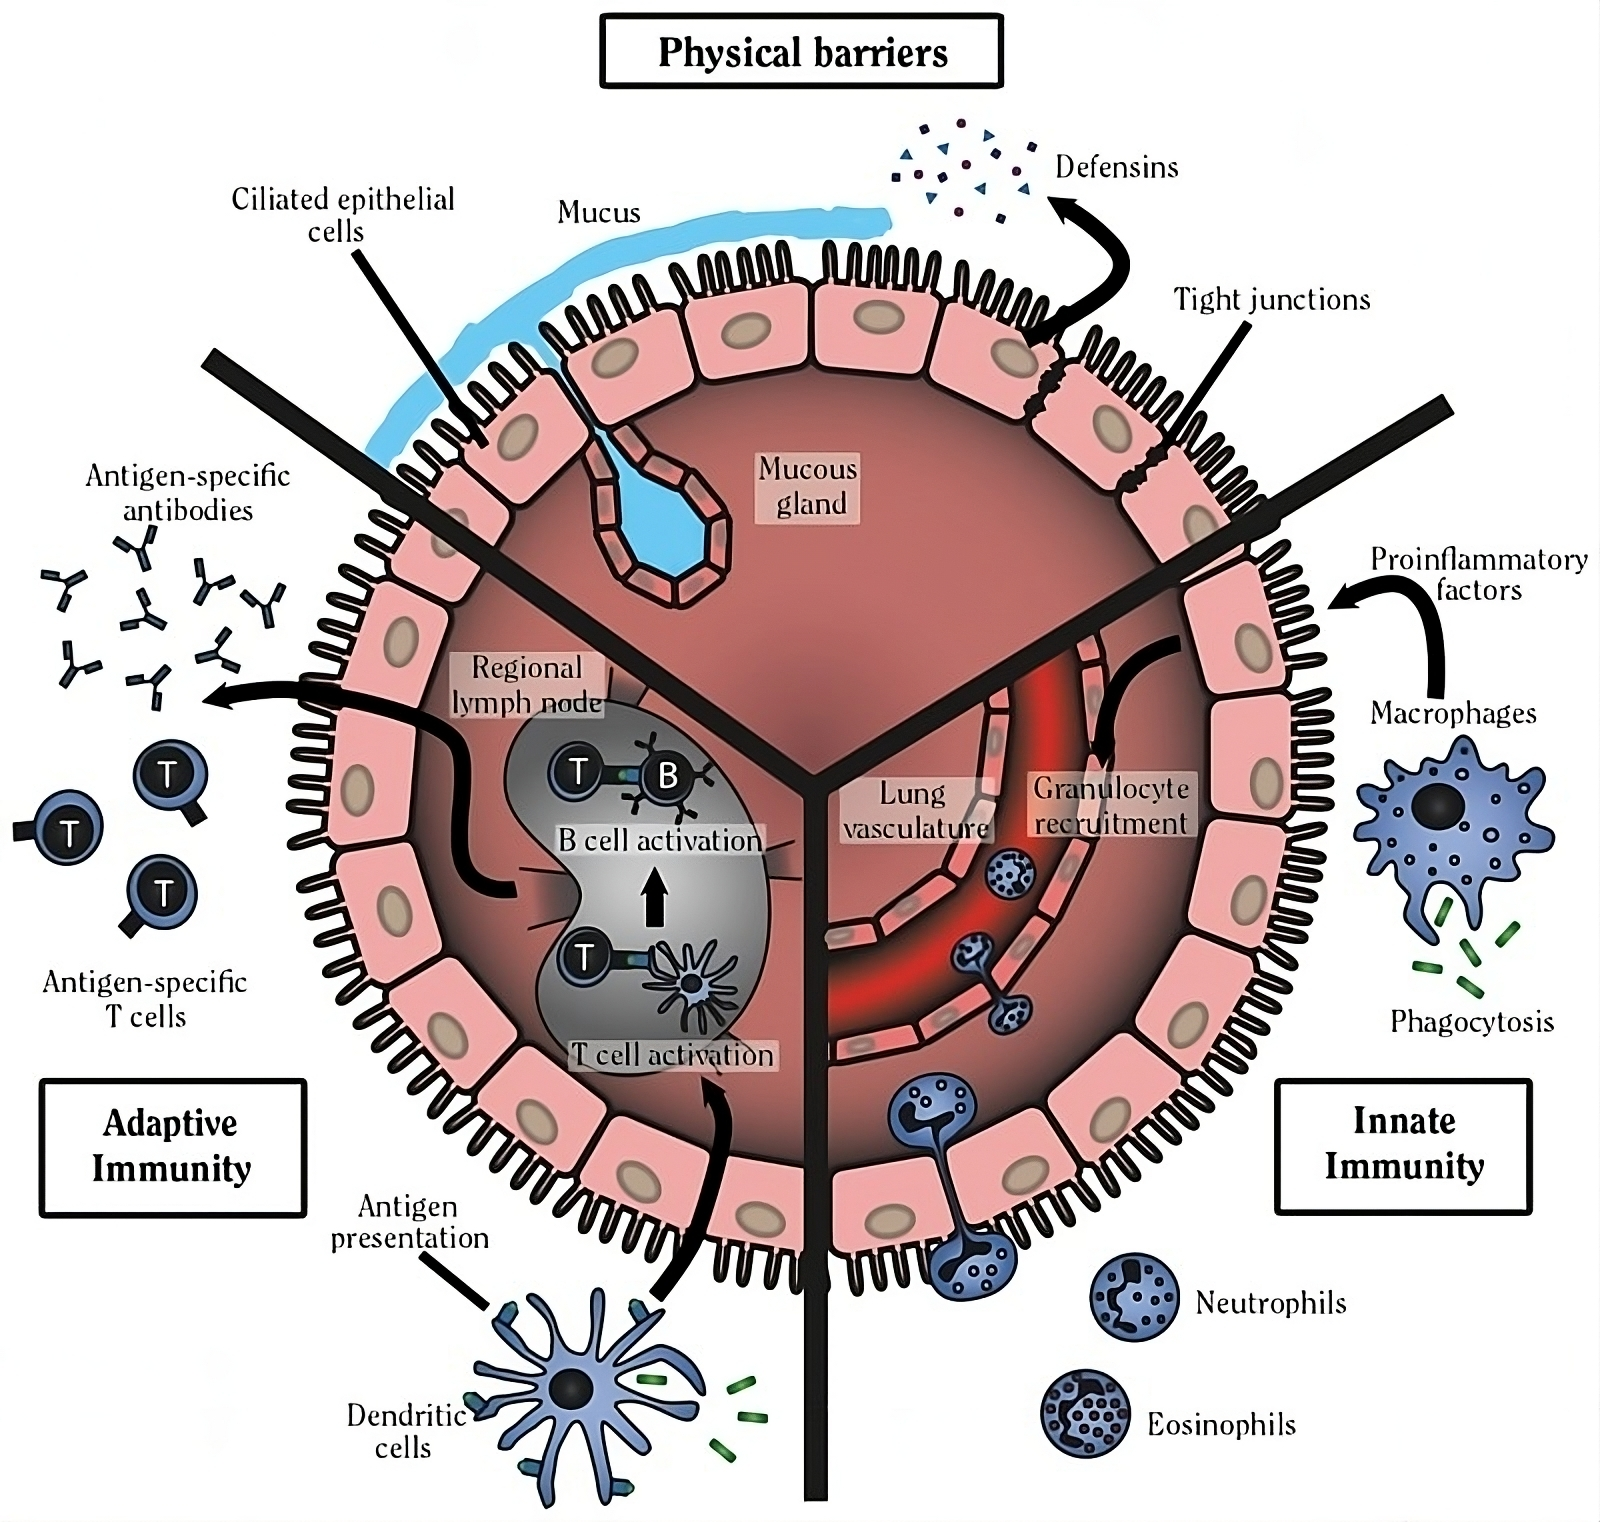
\includegraphics[width=0.9\textwidth]{images/Diagram_of_innate_and_adaptive_immunity.jpeg}
  \caption[Diagram of Innate and Adaptive Immunity]{Diagram showing physical barriers, innate immune cells (e.g., macrophages, dendritic cells, natural killer cells) and adaptive immune components (B and T cells) working together. Reproduced from Figure 10.5 in \emph{The Health Consequences of Smoking—50 Years of Progress: A Report of the Surgeon General} (2014) \cite{smoking2014}.}
  \label{fig:immunity}
\end{figure}
\noindent
\textbf{Adaptive Immunity (left)}\\
Acquired or adaptive immunity is the “slower but more targeted” defense. This branch takes days to weeks to develop a full, specific response upon initial exposure to a pathogen (or vaccine antigen). A key concept in adaptive immunity is the antigen, which is any substance, usually foreign (such as from a pathogen or vaccine), that triggers a specific immune response in the body. B cells play a crucial role by producing antibodies, which are proteins that bind to specific non-self antigens. These antibodies neutralize pathogens and tag them for destruction by immune cells such as phagocytes.
Higher concentrations of antibodies generally indicate a stronger immune response. T cells are also crucial and have several roles. They help coordinate the immune response (often referred to as helper T cells) and can directly kill infected cells (cytotoxic T cells). \glspl{tcr}, located on the surface of T cells and responsible for recognizing peptides presented by MHC I/II molecules, can be sequenced (see Figure~\ref{fig:TCR_profiling}) to determine which T cell clones are activated in response to a vaccine. A major advantage of adaptive immunity is that it “learns” from previous exposure, allowing for much faster and more powerful immune responses in the event of repeated infection. This ability to form memory also underlies how vaccines work \cite{janeway2001immunobiology}.

\begin{figure}[h]
  \centering
  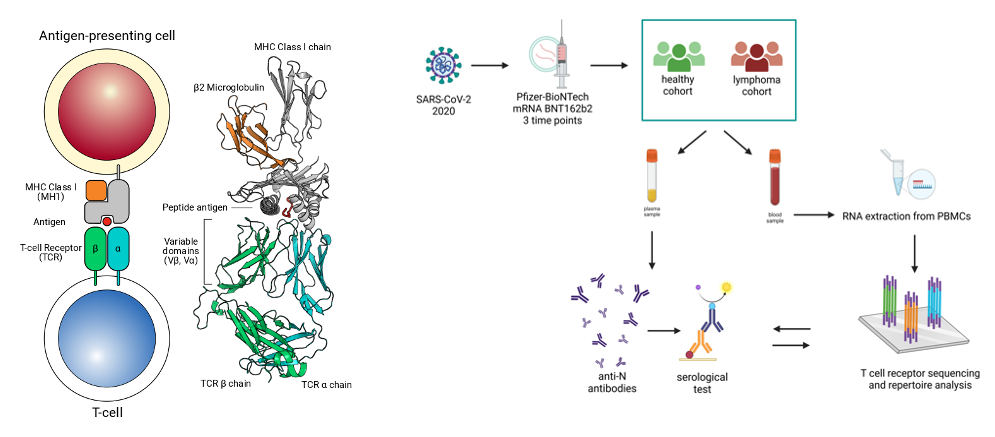
\includegraphics[width=1\textwidth]{images/TCR_profiling.png}
  \caption[ \gls{tcr} sequencing Workflow]{Schematic outline of how \gls{tcr} data is obtained from peripheral blood mononuclear cells (PBMCs) after vaccination. By extracting and profiling \gls{tcr} sequences, it becomes possible to identify which T cell clones expand in response to the vaccine. This information provides insights into the breadth (diversity) and depth (magnitude or intensity) of the adaptive immune response. (Left panel Adapted from Leem et al. (2018) \cite{Leem2018IMGTHLA}}
  \label{fig:TCR_profiling}
\end{figure}

\noindent
Together, these three pillars provide a robust defence system that is able to successfully fight off most infections. It is also this dynamic between innate and adaptive immunity that determines the degree of vaccine response. The innate branch prepares the way, while the adaptive branch provides targeted antibodies and memory cells. This context is important because the predictive models developed here integrate features from both the innate and adaptive immune systems. For example, innate markers such as cytokine levels and certain cell counts can provide early signals about the body's general readiness to respond. Meanwhile, adaptive markers, such as \gls{tcr} sequences of T cells, directly reflect the specific immune response that leads to antibody production after vaccination. Combining this data gives us a more complete picture of the immune landscape, allowing for better predictions of how effectively an individual will respond to the measles vaccine.

\subsection{Antibody Titers}
\label{sec:antibody_titers}
As mentioned above, antibody titers provide a quantitative measure of the concentration in the blood antibodies with a certain specificity, making them a reliable indicator of the immune system’s functional response against a pathogen \cite{plotkin2010correlates}. In essence, they reflect the “signal strength” of the response, with high titers indicating robust protection and low titers suggesting a weaker response. Antibody titers thus serve as a crucial biomarker for classifying vaccine responses into strong and weak responders.

\pagebreak
\section{Background in Computer Science}
\noindent
In this work, several key computer science concepts, primarily from machine learning, are employed to analyze and interpret multimodal biological data in predicting vaccine responses. Methodologies for addressing class imbalance, such as the \acrfull{smote}, and for understanding model predictions, like \acrfull{shap}, are more central to this work and will be detailed further in the methodology sections (Chapter~\ref{chap:methodology}).

\subsection{Classification}
Classification is a type of machine learning in which the goal is to assign a label or category to a sample, also called an instance or observation, which typically corresponds to one row in a dataset. In our case, a sample represents the biological data of a vaccinated individual. Each sample is described by multiple features (such as gene expression values or immune cell counts), and together these features place the sample in a high-dimensional space, where each axis corresponds to a specific feature of that sample.\\
\\
In the simplest case, we deal with binary classification, where there are only two possible outcomes. Here, those outcomes are: either the person responded to the vaccine (a responder), or they did not (a non-responder). The goal of the classification model is to learn from known examples, where the response is already labeled, and then use that knowledge to make predictions about new, unseen examples.\\
\\
For this scenario, you can think of classification as teaching a model to recognize biological patterns. For example, the model is trained on data like immune cell counts or gene expression from individuals whose vaccine response is already known. Over time, it learns to associate certain patterns in this data with responders or non-responders. Once trained, it can predict the response for new individuals based on their biological measurements.\\
\\
However, one important risk in training such models is called overfitting. Overfitting happens when a model becomes too good at memorizing the training data, including small details or noise that don’t apply generally. This means it might perform very well on the training set but fail to make accurate predictions on new, unseen data. Instead of learning general patterns, it has simply memorized specific examples. A well-designed classification model aims to avoid this by focusing on patterns that are likely to hold true across different datasets, not just the one it was trained on.

\subsection{Classifiers}
Classifiers are algorithms or models used to implement classification tasks. This thesis utilizes several classifiers, each selected for their unique strengths and applicability to biological data:
\begin{itemize}
    \item \textbf{Logistic Regression}: A statistical model used for binary classification that estimates the probability of a sample belonging to a class using a sigmoid function. This model may perform poorly when the true relationship between features and the target is highly non-linear or complex.
    \item \textbf{Decision Trees}: Intuitive models that split data into subsets based on feature values, forming a tree of decision rules. They are easy to interpret and visualize, and handle both numerical and categorical data. However, they are prone to overfitting, especially with deep trees or noisy data.
    \item \textbf{Random Forest}: An ensemble method that constructs multiple decision trees and combines their predictions to improve generalization. This makes them more robust and accurate than a single decision tree and less sensitive to overfitting. A disadvantage is that they are less interpretable and more computationally intensive than individual trees.
    \item \textbf{Support Vector Machine (SVM)}: A classifier that finds the optimal boundary (hyperplane) that maximally separates different classes. SVMs are effective in high-dimensional spaces and with clear margins of separation. On the other hand, they can be slow to train and are also less effective when classes are not well-separated.
    \item \textbf{Gaussian Naive Bayes}: A probabilistic classifier based on Bayes’ theorem that models continuous features using Gaussian distributions and assumes feature independence. It is highly efficient and performs well on small datasets or when the independence assumption is approximately valid. However, its performance can degrade when features are strongly correlated.
\end{itemize}

\subsection{Verification of Classifiers}
Verification of classifiers involves assessment of their predictive capabilities on unseen data to ensure reliability and generalization, thus avoiding overfitting. Techniques used include:
\begin{itemize}
\item \textbf{Cross-Validation}: This technique repeatedly partitions the dataset into subsets, training models on a majority of subsets and validating performance on the remaining subset. It robustly estimates how models perform on unseen data.
\item \textbf{Permutation Testing}: A statistical method where the labels of the dataset are randomly shuffled multiple times, and the model performance is evaluated on these permuted datasets. It determines if the model's observed predictive performance is significantly better than random chance.
\end{itemize}

\subsection{Performance Metrics}
Performance evaluation metrics are crucial for understanding and quantifying classifier effectiveness. These metrics rely on counts of correct and incorrect predictions, categorized as follows:
\begin{itemize}
\item \textbf{True Positives (TP)}: Correctly identified positive cases.
\item \textbf{True Negatives (TN)}: Correctly identified negative cases.
\item \textbf{False Positives (FP)}: Incorrectly identified negative cases as positive (Type I error).
\item \textbf{False Negatives (FN)}: Incorrectly identified positive cases as negative (Type II error).
\end{itemize}
\noindent
\textbf{Precision} measures the accuracy of positive predictions, critical when false positives are costly:
\[
\textbf{Precision} = \frac{\text{TP}}{\text{TP} + \text{FP}}
\]
\noindent
\textbf{Recall} (or sensitivity) assesses how effectively actual positives are identified, essential when missing positives is especially detrimental:
\[
\textbf{Recall} = \frac{\text{TP}}{\text{TP} + \text{FN}}
\]
\noindent
\textbf{Accuracy} is one of the most basic evaluation metrics in classification and measures the overall proportion of correctly predicted samples. It is calculated as:
\[
\textbf{Accuracy} = \frac{\text{TP} + \text{TN}}{\text{TP} + \text{TN} +  \text{FP} + \text{FN}}
\]
While easy to interpret, accuracy can be misleading in datasets where the classes are imbalanced. For example, if 90\% of samples belong to one class, a model that always predicts that majority class will achieve 90\% accuracy, even if it completely fails to recognize the minority class.\\
\\
\noindent
\textbf{Balanced Accuracy} offers a more informative view in such scenarios. It equally weights performance across classes by averaging recall for each class:
\[
\textbf{Balanced Accuracy} = \frac{1}{2} \left(\frac{\text{TP}}{\text{TP} + \text{FN}} + \frac{\text{TN}}{\text{TN} + \text{FP}}\right)
\]
This metric ensures that the evaluation accurately reflects the classifier’s ability to correctly identify instances across both majority and minority classes, making it highly relevant for the imbalanced biological data analyzed in this thesis.

\subsection{\acrfull{pca}}
\acrfull{pca} is a dimensionality reduction technique used to simplify complex datasets. \acrshort{pca} works by transforming a set of potentially correlated variables into a new set of uncorrelated variables called \textbf{principal components}. These principal components represent linear combinations of the original features and are ordered such that the first principal component captures the largest variance from the dataset. Each subsequent component captures progressively less variance and remains orthogonal (uncorrelated) to all preceding components. Thus, when \acrshort{pca} is applied to a dataset with $n$ features, it generates $n-1$ principal components, each accounting for a decreasing proportion of the dataset's total variance.\\
\\
In the context of this thesis, \acrshort{pca} serves multiple critical purposes. First, it reduces redundancy in the data by projecting correlated features into a smaller number of uncorrelated principal components. This transformation simplifies the dataset and can improve predictive performance by mitigating issues such as multicollinearity. Second, \acrshort{pca} it can facilitate visualization by projecting high-dimensional data onto a two dimensional space. Such visualization helps to reveal inherent patterns, clusters, and potential outliers, thus providing clearer insights into the dataset’s underlying structure, which would otherwise be difficult to discern in high-dimensional feature spaces.
%%%%%%%%%%%%%%%%%%%%%%%%%%%%%%%%%%%%%%%%%%%%%%%%%%%%%%%%%%%%%%%%%%%%%%%%%%%%%%%%%%%%%%%%%%%%%%%%%%%%%%%%%%%%%%%%%%%%%%%%%%%%%%%%%%%%%%%%%%%%%%%%%






\chapter{Related Work}
%%%%%%%%%%%%%%%%%%%%%%%%%%%%%%%%%%%%%%%%%%%%%%%%%%%%%%%%%%%%%%%%%%%%%%%%%%%%%%%%%%%%%%%%%%%%%%%%%%%%%%%%%%%%%%%%%%%%%%%%%%%%%%%%%%%%%%%%%%%%%%%%%
Integrating diverse patient data, such as omics, imaging, and clinical information, is crucial for personalized medicine. Various computational approaches exist to fuse these multimodal data types to enhance predictive modeling and derive deeper biological insights \cite{Qoku2023Multimodal}.\\
\\
Feature-Level (Early) Fusion Classifiers combine all raw features from different modalities into a single, comprehensive input vector. This consolidated vector is then fed into a single classifier, which can be a traditional machine learning algorithm or a deep neural network. For instance, studies have successfully applied early fusion by combining radiology and pathology image features to improve tumor grade predictions. While straightforward, early fusion may not optimally handle modality-specific structures or extensive missing data within individual modalities \cite{Qoku2023Multimodal}. Intermediate Fusion Neural Networks process each data modality through dedicated subnetworks to learn initial, modality-specific representations. These learned latent representations are then merged at an intermediate layer within the neural network's architecture. This mid-level fusion strategy benefits from initial modality-specific learning while subsequently capturing interactions through a joint representation. Multi-branch deep neural networks, often employing specialized components like convolutional neural networks for images, are common in this approach. An example includes cancer studies using separate CNN branches for histopathology and radiology images, with their outputs then fused to predict survival. This method is often highly effective for modeling complex cross-modal relationships in biomedical tasks \cite{Qoku2023Multimodal}. Decision-Level (Late) Fusion Approaches involve training independent models on each data modality separately. Each model generates its own prediction or decision, and these individual outputs are then combined in a final step to form a unified decision. The combination can be as simple as averaging predictions or as sophisticated as using a meta-learner. This strategy offers flexibility, allowing for different model types to be used for each modality, and is robust to missing data from specific modalities since each model operates independently. For example, researchers have built separate predictive models for histology, imaging, and genomic biomarkers, then integrated their combined risk scores to enhance overall survival prediction \cite{Qoku2023Multimodal}. In this study, this concept was explored by building independent models for different data types within a single cohort, and then combining their predictions through a consensus mechanism.\\
\\
Beyond primary methods, Autoencoder-Based Joint Representation uses autoencoders (e.g., VAEs) to create a shared latent space across modalities for prediction. Attention-Based and Transformer Models (like MCAT) employ attention mechanisms for dynamic cross-modal information alignment, enhancing performance and interpretability. Other approaches include Ensemble \& Stacking, which combine predictions from single-modality models. Probabilistic Graphical Models define relationships between multimodal variables. Lastly, Graph Neural Networks (Graph-Based Fusion) treat multimodal data as a network to fuse information and incorporate domain knowledge \cite{Qoku2023Multimodal}.\\
\\
Implementing these multimodal classifiers comes with challenges that need to be addressed. Recent advances in biomedical machine learning have increasingly emphasized both the need to address class imbalance and the importance of interpretability in predictive models. Techniques such as \acrfull{smote} and \acrfull{shap} have gained prominence in this context.\\
\\
In the last five to seven years, a limited number of studies have explored pipelines combining \acrshort{smote} and \acrshort{shap}. For instance, \acrshort{smote} has been used to balance data distributions prior to model training, followed by \acrshort{shap} to identify key predictive features in Parkinson’s disease diagnosis (31 individuals, 195 voice samples) and cardiac arrhythmia classification (48 recordings) \cite{sofi2025parkinsons, xiao2024interpretable}. A similar strategy was applied in cancer informatics, where Kim (2025) used \acrshort{smote} to improve minority-class representation and \acrshort{shap} to engineer a reduced, interpretable feature space for appendiceal cancer prediction \cite{kim2025shap}. While these studies demonstrate the feasibility of the \acrshort{smote}+\acrshort{shap} pairing, they are typically situated in domains with lower dimensionality or larger sample sizes, and they rarely address the issue of instability across data splits.\\
\\
Initially, the thesis explored consensus modeling techniques to mitigate instability in model performance on small, multimodal datasets. However, it became apparent that standard consensus models proved insufficiently robust. This motivated the development of a revised pipeline which explicitly incorporates repeated data partitioning. In this approach, models are trained and \acrshort{shap}-based interpretations are generated for each data split. Feature importance is then aggregated across reliable models. The primary goal of this strategy is to counteract the known instabilities associated with high-dimensional, low-sample-size data while preserving both predictive power and interpretability. This design was also driven by recent literature warning that a naive application of \acrshort{smote} may distort downstream model interpretation. Gholampour (2023) found that oversampling altered \acrshort{shap} feature rankings in stroke prediction models to the extent that spurious features replaced clinically validated ones \cite{gholampour2024impact}. This shows the necessity of careful methodological design when combining data augmentation and model explanation techniques.\\
\\
Therefore, while the use of \acrshort{smote} and \acrshort{shap} is slowly gaining traction in biomedical AI, their combined use in the context of small, heterogeneous datasets with repeated-split validation is an area that merits further comprehensive investigation. This thesis aims to provide insights into this challenging area through a deliberately cautious and stability-driven implementation, seeking to gain results that are not only predictive, but also more robust and biologically meaningful.

%%%%%%%%%%%%%%%%%%%%%%%%%%%%%%%%%%%%%%%%%%%%%%%%%%%%%%%%%%%%%%%%%%%%%%%%%%%%%%%%%%%%%%%%%%%%%%%%%%%%%%%%%%%%%%%%%%%%%%%%%%%%%%%%%%%%%%%%%%%%%%%%%






\pagebreak
\chapter{Data Description and Preprocessing}
%%%%%%%%%%%%%%%%%%%%%%%%%%%%%%%%%%%%%%%%%%%%%%%%%%%%%%%%%%%%%%%%%%%%%%%%%%%%%%%%%%%%%%%%%%%%%%%%%%%%%%%%%%%%%%%%%%%%%%%%%%%%%%%%%%%%%%%%%%%%%%%%%
\noindent
In this chapter, I provide an overview of the measles dataset used in this study and outline the preprocessing steps required to prepare the data for analysis. The dataset integrates multiple biological modalities (including cytokine profiles, cytometry measurements, antigen-specific clonal breadth and depth of T cell receptors, and \acrshort{rna} sequencing data) to capture various aspects of the immune response to the measles vaccine. Additionally, I explain how response labels were assigned based on antibody titer trajectories, which serve as a key indicator of vaccine effectiveness.

\section{Label Assignment Strategy}
\noindent
Defining a successful immune response following vaccination can be complex, particularly in the presence of pre-existing immunity due to prior exposure or vaccination. To capture the dynamics of antibody levels over time, this study utilizes antibody titer measurements taken at four time points: at baseline (pre-vaccination) and at 21, 150, and 365 days following inoculation.\\
\\
The original source study \cite{bartholomeus2020transcriptomic} employed a hierarchical clustering method based on these longitudinal IgG titer evolution patterns to classify subjects into more granular response groups, effectively avoiding potentially biased arbitrary cut-off values. The study identified four primary response clusters: High Ab, Low Ab, Long response, and Peak response. For visualization purposes, these original classifications were consolidated into three categories displayed in Figure~\ref{fig:titer_original_label}: \texttt{responder} (combining Long response, and Peak response), \texttt{no response - high ab} (representing individuals with high baseline antibody levels who did not show a significant increase), and \texttt{no response - low ab} (representing individuals with low baseline levels who also did not show a significant increase).\\
\\
Figure~\ref{fig:titer_original_label} displays the antibody titer trajectories for each subject over the four measured time points, with lines colored according to these response categories. The x-axis displays the time points at which measurements were taken: Day 0 (post-vaccination), Day 21, Day 150, and Day 365.The y-axis indicates the antibody titer level. Each line follows the trajectory of an individual subject. Subplots A–C each show per-subject trajectories for one response group: (A) responders, (B) no response – low ab, and (C) no response – high ab. Panel D combines all three groups for comparison.\\
\\
The visualization highlights distinct dynamic patterns associated with these categories. Subjects classified as \texttt{responder} typically exhibit a pronounced increase in antibody titers following vaccination, primarily between Day 0 and Day 21, before a gradual decline. Conversely, the non-responder groups generally show more stable trajectories. The \texttt{no response - high ab} group maintains high titers throughout, while the \texttt{no response - low ab} group maintains low titers, neither showing the significant early boost characteristic of the responders. This visual distinction shows how pre-existing titers can influence the observed response pattern, where individuals with high baseline levels may not show a significant increase upon re-vaccination as their immune system is already primed and maintaining high antibody production.\\
\begin{figure}[h!]
  \centering
  \hspace*{-0.5cm}
  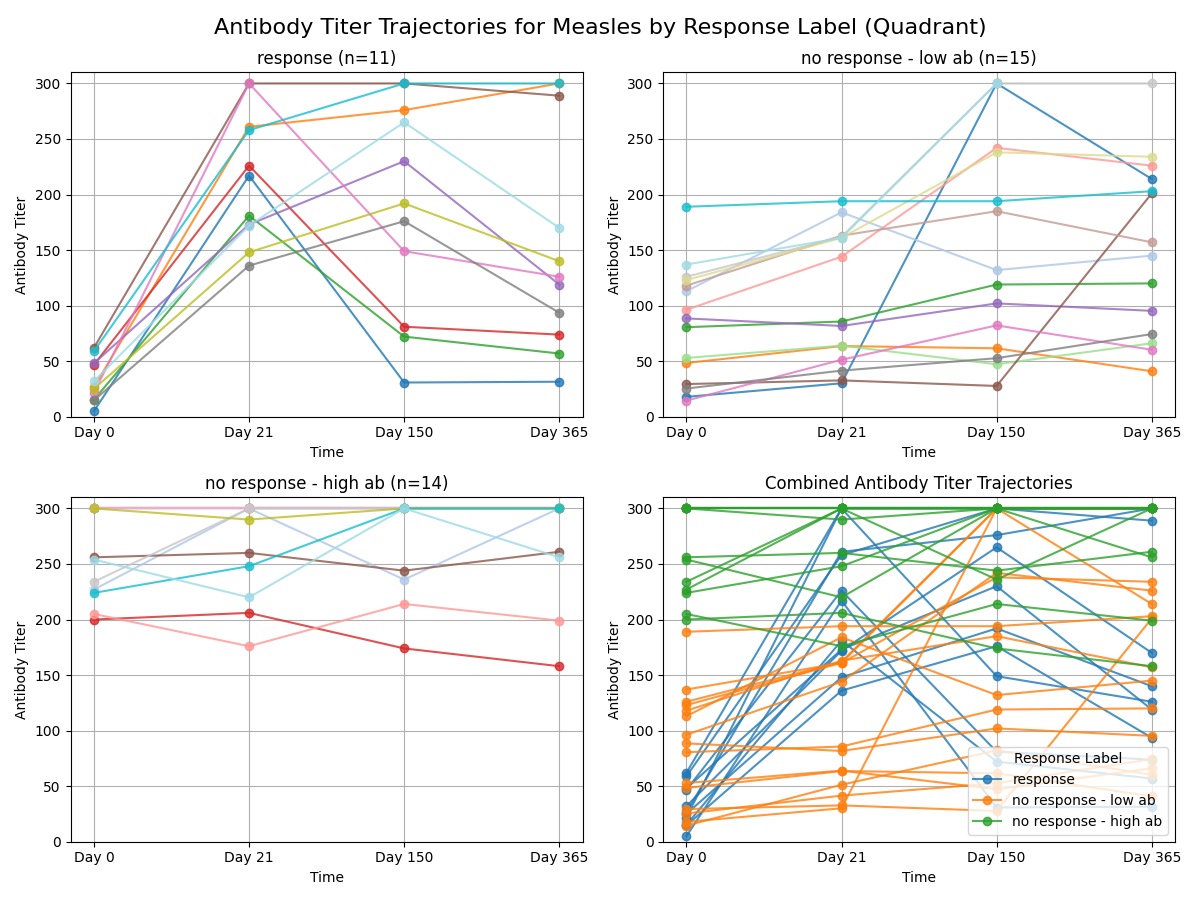
\includegraphics[width=1.05\textwidth]{images/Antibody_Titer_Trajectories_for_Measles_by_Original_Label_(Quadrant).png}
  \caption[Antibody Titer Trajectories by Original Label (Quadrant)]{Antibody titer trajectories for each subject, colored by the original qualitative labels (quadrant). The plots illustrate variations in antibody responses, suggesting distinct patterns. Responders typically display a sharp initial increase followed by gradual decline, while non-responders tend to maintain consistently low or high titers.}
  \label{fig:titer_original_label}
\end{figure}
\\
\noindent
For the initial stages of predictive modeling in this thesis, we simplified the outcome variable to a binary classification: \texttt{responder} and \texttt{non-responder}. This simplification was made to create a more straightforward prediction task, focusing on the presence or absence of a successful boosting effect. Based on the visually distinct boosting pattern observed in Figure~\ref{fig:titer_original_label}, a subject was defined as a \texttt{responder} if their antibody titer increased by at least 120 mIU/mL from Day0 to Day21. This threshold reflects a widely accepted criterion for achieving protective immunity against measles \cite{chen1990measles} and corresponds to capturing the significant initial titer increase characteristic of the \texttt{responder} group in the figure. Subjects from both the \texttt{no response - high ab} and \texttt{no response - low ab} categories in Figure~\ref{fig:titer_original_label} were combined into the \texttt{non-responder} class for the binary prediction task, as neither group exhibited this defining boosting signature despite their different baseline states.

\section{Dataset Construction and Preprocessing}
\subsection{Cytokines}
The cytokine data consists of direct measurements of the concentrations of various cytokines and related soluble factors in patient samples. The dataset contains quantified levels for each cytokine (CMV.Status, EBV.Status, HSV1\_2.Status, HHV6.Status, EGF, FGF-2, Eotaxin, TGF-a, GCSF, Flt3 Ligand, GM-CSF, Fractalkine, IFNa2, IFNg, GRO, IL-10, MCP3, IL12-p40, MDC, IL12-p70, IL-13, IL-15, sCD40L, IL17A, IL1Ra, IL1a, IL-9, IL-1b, IL-2, IL-5, IL-6, IL-7, IL-8, IP-10, MCP-1, MIP1a, MIP1b, TNFa, TNFb, VEGF) across different vaccinees, along with their CMV and viral status. Unlike the \acrshort{rna} data, which required a multi-step process to derive module scores from raw read counts, the cytokine data represents the empirically measured values. Therefore, it did not need a complex data construction or preprocessing workflow to obtain the presented concentrations.

\subsection{Cytometry}
The cytometry data consists of various hematological parameters, including \acrfull{wbc}, \acrfull{rbc}, \acrfull{hgb}, \acrfull{hct}, \acrfull{plt}, and the percentages of lymphocytes (\%\acrshort{lym}), monocytes (\%\acrshort{mon}), and granulocytes (\%\acrshort{gra}). These measurements were collected at multiple time points post-vaccination (Day 0 (pre-vaccination), Day 21, Day 180, and Day 365). For the analysis presented here, only the baseline values obtained at Day 0 were utilized. Similar to the cytokine data, the cytometry data comprises direct quantitative measurements and did not require a complex data construction or preprocessing workflow beyond the selection of the Day 0 time point.

\subsection{\gls{tcr} Breadth and Depth Metrics}
Analyzing the adaptive immune response, especially T cells, through characterization of the \gls{tcr} repertoire reveals critical insights into the diversity and strength of responses to specific antigens. This study focused on metrics describing the T cell response specific to the measles pathogen, as individuals were vaccinated with the \gls{mmr} vaccine containing a live-attenuated measles virus strain.\\
\\
To identify \gls{tcr} clones likely involved in this measles-specific response, the ImmuneWatch DETECT tool \cite{ImmuneDetectDocs} was utilized. This tool has been shown to be the best performing method for TCR-epitope binding predictions, as demonstrated by its superior results in the IMMREP23 benchmark \cite{benchmarking_paper_2024}. DETECT analyzes \gls{tcr} sequencing data. It predicts which \gls{tcr}  sequences in a sample are specific to a pathogen or antigen using a large database of known pathogen-associated \gls{tcr}s. Once the measles-specific \gls{tcr} clones were identified using DETECT, two key metrics were calculated: Breadth and Depth.\\
\\
\textbf{Breadth} quantifies the diversity of the T cell response. It measures the variety of unique T cell clones in a sample. Each distinct \gls{tcr} sequence is a unique clone. Higher breadth indicates a more diverse repertoire and broader participation of different T cell clones in the immune response. The Breadth metric was computed from the DETECT output. It's reported as the fraction of unique \gls{tcr} sequences specific to measles. These are presented separately for alpha-beta (ab) and gamma-delta (gd) \gls{tcr}s, in the "fraction\_sequences\_ab" and "fraction\_sequences\_gd" columns of the dataset.\\
\\
\textbf{Depth}, on the other hand, quantifies the magnitude or abundance of the predicted measles-specific T cell response. It reflects how much individual predicted measles-specific clones have expanded upon encountering the antigen. Depth measures the abundance of these expanded clones. This metric is computed from the predicted measles-specific \gls{tcr} sequences identified by DETECT and the abundance data from the full repertoire. The "uniqueMoleculeFraction\_ab" and "uniqueMoleculeFraction\_gd" columns represent this. They show the frequency or proportion of molecules associated with these unique predicted sequences, indicating clonal abundance within the predicted response. Higher depth for a clone means it expanded more within this predicted repertoire, showing a stronger response from that T cell group.\\
\\
Together, breadth and depth, provide a comprehensive view of the T cell immune response, characterizing both the diversity of the responding clones and the magnitude of their expansion.

\subsection{Bulk \acrshort{rna} Sequencing Data}
\label{subsec:rna_data_construction}
The \acrshort{rna} data utilized in this study was constructed from two primary sources. The first source comprised raw \acrshort{rna} read counts, provided in a matrix format where rows represented individual patients and columns corresponded to detected genes. The second source was a curated list of gene modules. These modules, known as BloodGen3 \cite{Altman2021BloodGen3}, group genes based on co-expression patterns identified across 985 unique blood transcriptome profiles from studies of diverse immune conditions. Each module also has an assigned biological function.\\
\\
To transform the raw gene-level read counts into a more interpretable and lower-dimensional representation, module scores were calculated. This process involved iterating through each defined gene module. For a given module, the read count data for its member genes were extracted across all patients. Before calculating module scores, the raw \acrshort{rna} read counts were first normalized using DESeq2 to account for library size and \acrshort{rna} composition differences between samples. Using these normalized gene expression values helps ensure that differences in gene-level expression scales do not disproportionately influence the module score. For further information on the DESeq2 normalization method \cite{love2014deseq2}. Subsequently, a single representative score for each module in each patient was derived by calculating the first principal component of the standardized expression values for the genes within that module using \gls{pca}. The resulting module score encapsulates the overall activity or expression pattern of the gene set comprising the module within each patient sample. This transformation yields a dataset where each row represents a patient and each column represents the calculated score for a specific gene module.

\section{Correlation Analysis Within Individual Datasets}
\label{sec:correlation_analysis_within_individual_datasets}
\noindent
In an initial exploratory phase, \acrfull{pca} was performed to understand the structure and dimensionality of the feature sets, specifically to investigate potential redundancy and correlations among features. \gls{pca} was applied to the full feature set, with a close look at the cytokines dataset. The analysis revealed that the first 10 principal components captured the majority of the variance within the data. This suggests that much of the dataset's information can be summarized in fewer dimensions, indicating a high degree of redundancy among features. Identifying these correlations is important, as it's a known challenge in high-dimensional data that can affect model interpretation and the stability of feature importance estimates. This observation also suggested that similar correlations might exist in the other datasets. These preliminary findings underline the challenges of high dimensionality and feature redundancy  that need to be addressed in subsequent predictive modeling efforts.\\
\\
Subsequently, correlation analysis was performed to examine the relationships between variables within each data source. As said earlier, the study comprises five distinct datasets capturing various aspects of the immune response: cytokines, cytometry, clonal breadth (\gls{tcr} metrics), clonal depth (\gls{tcr} metrics), and \acrshort{rna} data. Given the unique nature of the features captured by each modality, correlation analysis was conducted independently for each dataset. This approach enabled the identification of relationships within each data modality, which supported later clustering and feature selection steps for downstream modeling.

\subsection{Methodology}
\noindent
In this analysis, highly correlated features are grouped using hierarchical clustering. First, a pairwise Pearson correlation matrix is computed from the data. This correlation matrix is then used for hierarchical clustering of the features, performed by the \texttt{pheatmap} package \cite{pheatmap_package}. The output of \texttt{pheatmap} includes a heatmap visualizing the correlation matrix and a dendrogram representing the clustering results. To define modules, or clusters, of features, this dendrogram is cut at a fixed height corresponding to a specific number of clusters ($k$). The \texttt{cutree} function in R is used to obtain cluster assignments based on the desired number of clusters. While visualization functions from the \texttt{WGCNA} package \cite{WGCNA}, such as \texttt{plotDendroAndColors}, are used to display the dendrogram and assigned module colors, the module assignment itself is derived from cutting the \texttt{pheatmap}-generated hierarchical clustering dendrogram at a predetermined number of clusters. The resulting dendrogram with module assignments is provided in the appendix. This approach groups features that exhibit similar correlation patterns across the samples.

\subsection{Cytokine Data}
\begin{figure}[h!]
  \centering
  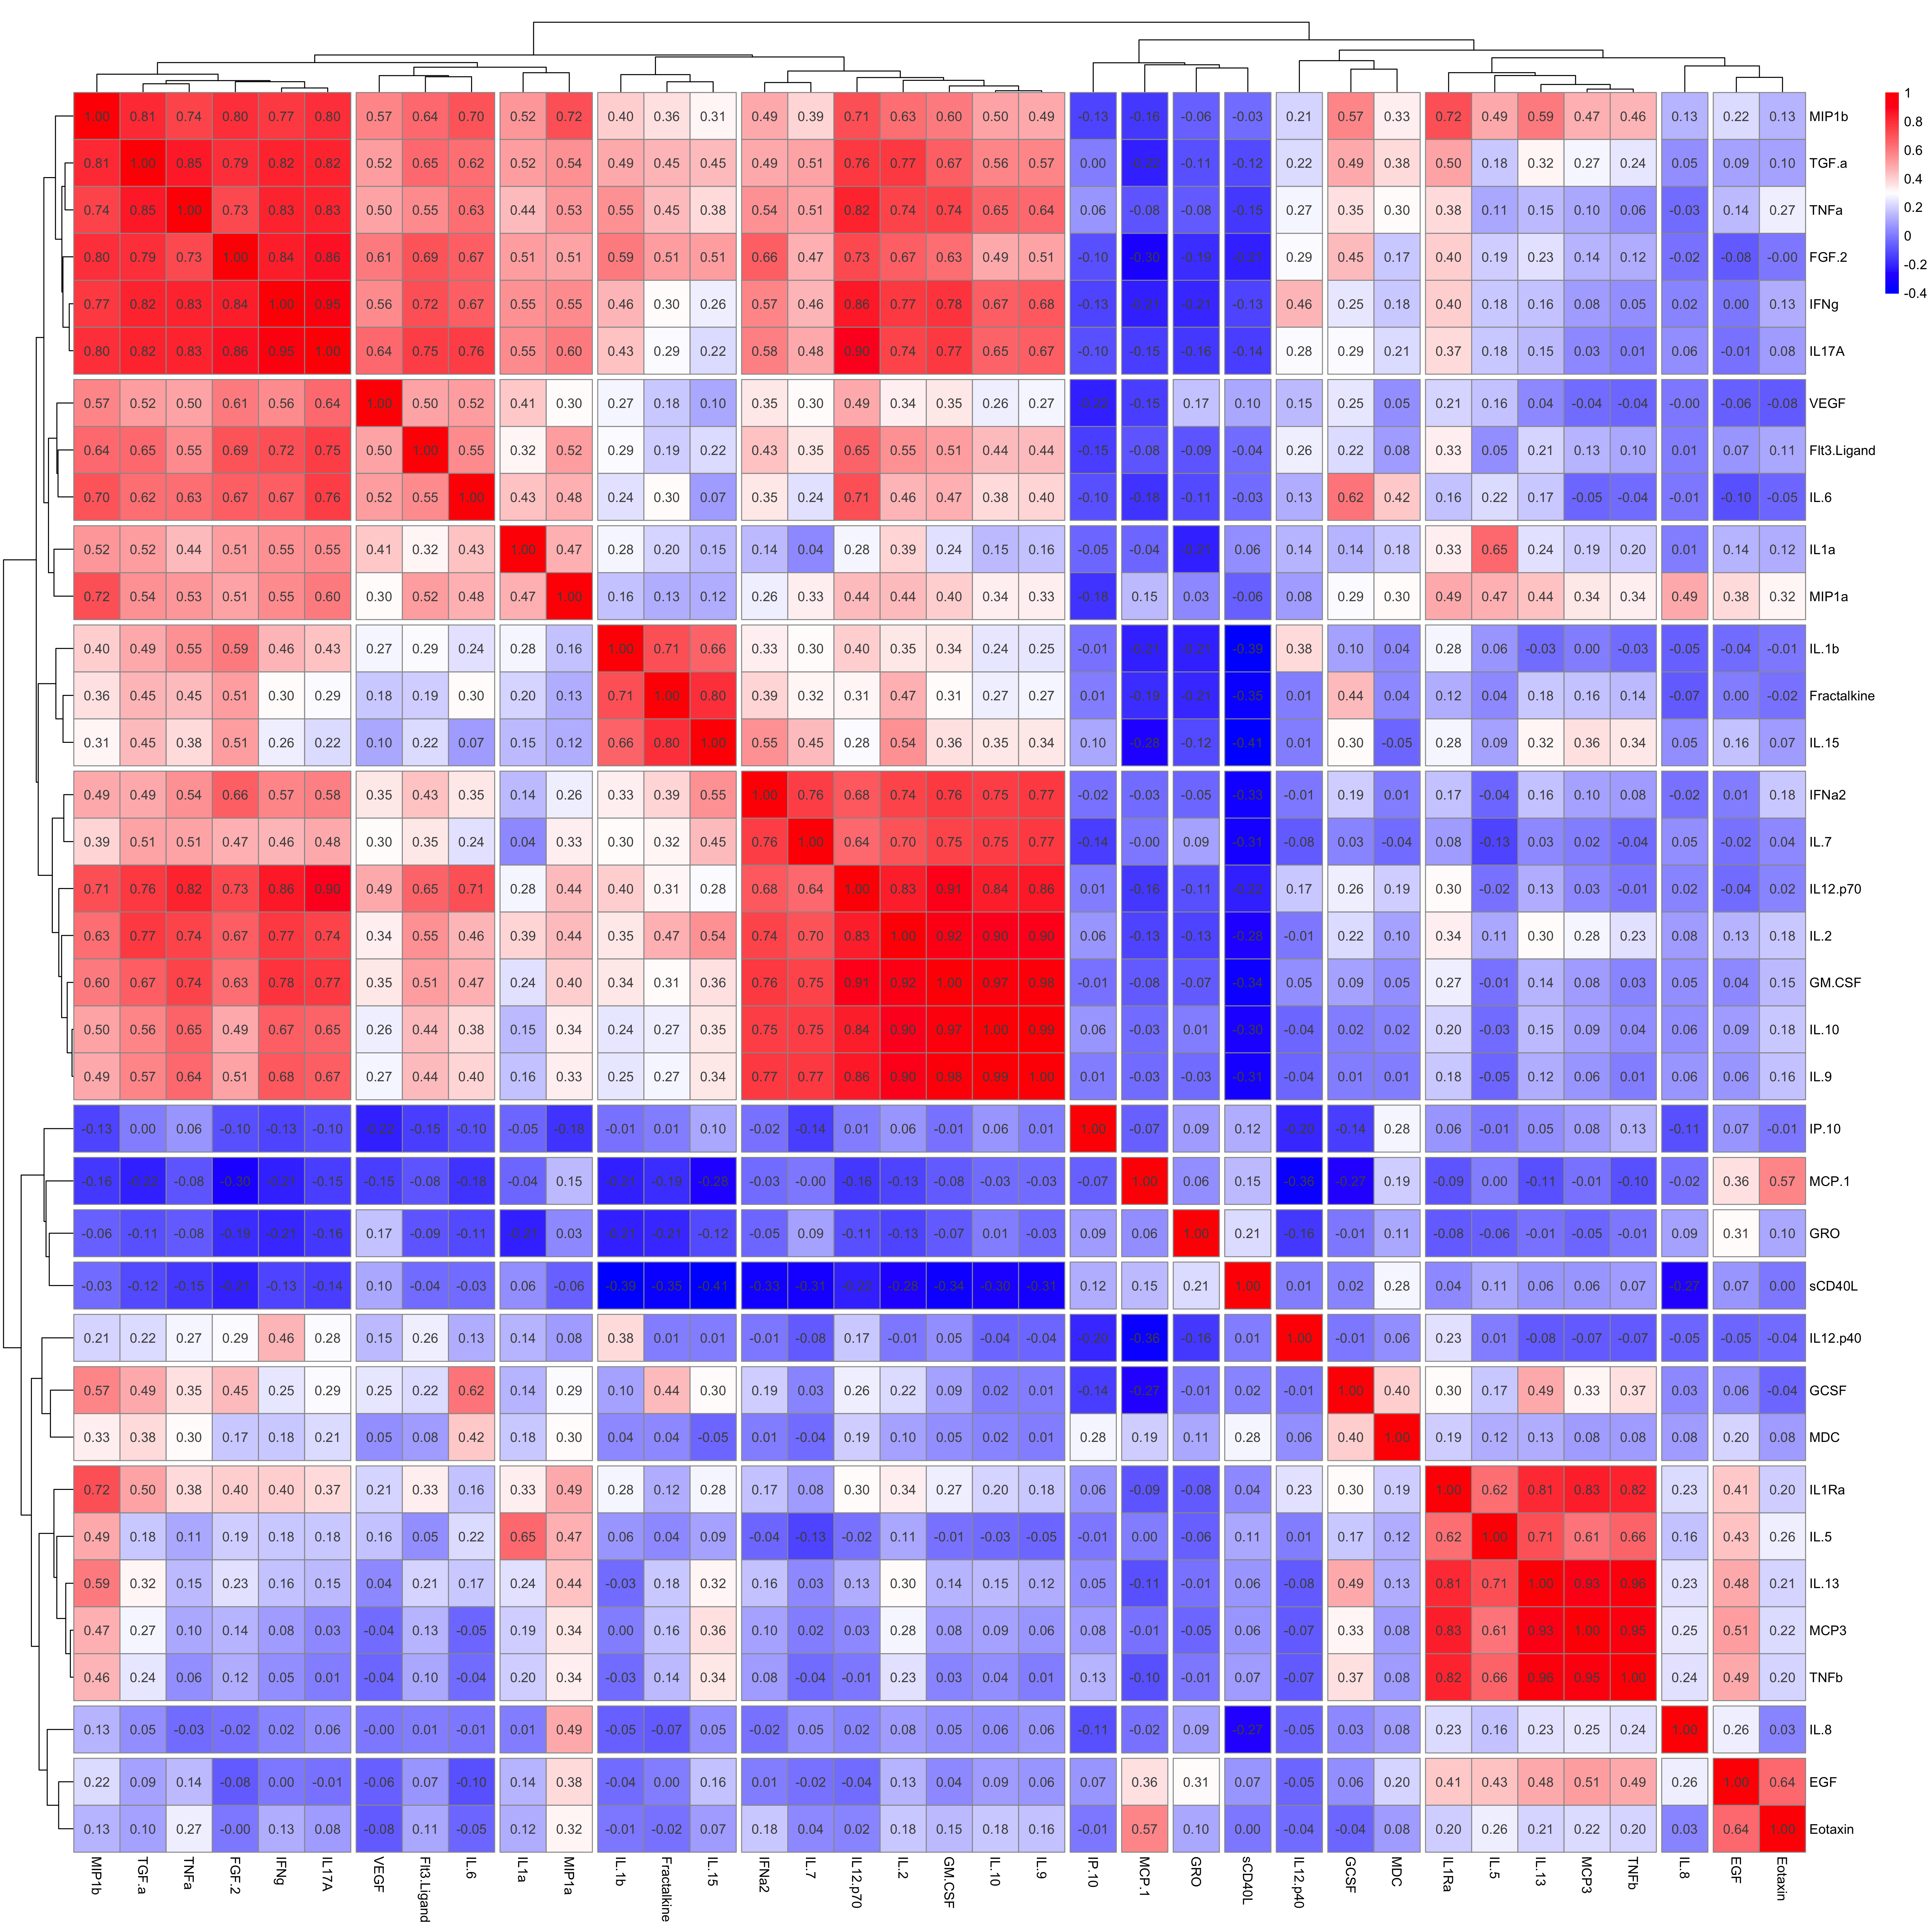
\includegraphics[width=0.8\textwidth]{images/Cytokine_euclidean_distance.png}
  \caption[cytokines data correlations]{Correlation heatmap of the cytokine data using hierarchical clustering.}
  \label{fig:cytokine_heatmap}
\end{figure}
\noindent
The following cytokine clusters were obtained from the hierarchical clustering analysis. The clustering reveals groups of cytokines with high inter-correlation, suggesting potential co-regulation or shared functional pathways. (For the corresponding dendrogram, refer to Figure~\ref{fig:Cytokines_features_clustering_cut_colors} in Appendix~\ref{appendix:cytokine_features_clusterings}).

\begin{table}[h!]
    \centering
    \begin{tabular}{ll}
        \textbf{Cluster 1:} & MIP1$\beta$, TGF-$\alpha$, TNF-$\alpha$, FGF-2, IFN-$\gamma$, IL17A. \\
        \textbf{Cluster 2:} & VEGF, Flt3 Ligand, IL-6. \\
        \textbf{Cluster 3:} & IL1$\alpha$, MIP1$\alpha$. \\
        \textbf{Cluster 4:} & IL-1$\beta$, Fractalkine, IL-15. \\
        \textbf{Cluster 5:} & IFN$\alpha$2, IL-7, IL12-p70, IL-2, GM-CSF, IL-10, IL-9. \\
        \textbf{Cluster 6:} & IL1Ra, IL-5, IL-13, MCP3, TNF$\beta$. \\
        \textbf{Cluster 7:} & GCSF, MDC. \\
        \textbf{Cluster 8:} & EGF, Eotaxin.
    \end{tabular}
    \caption{Cytokine Clusters}
    \label{tab:cytokine_clusters}
\end{table}


\subsection{Cytometry Data}

\begin{figure}[H]
  \centering
  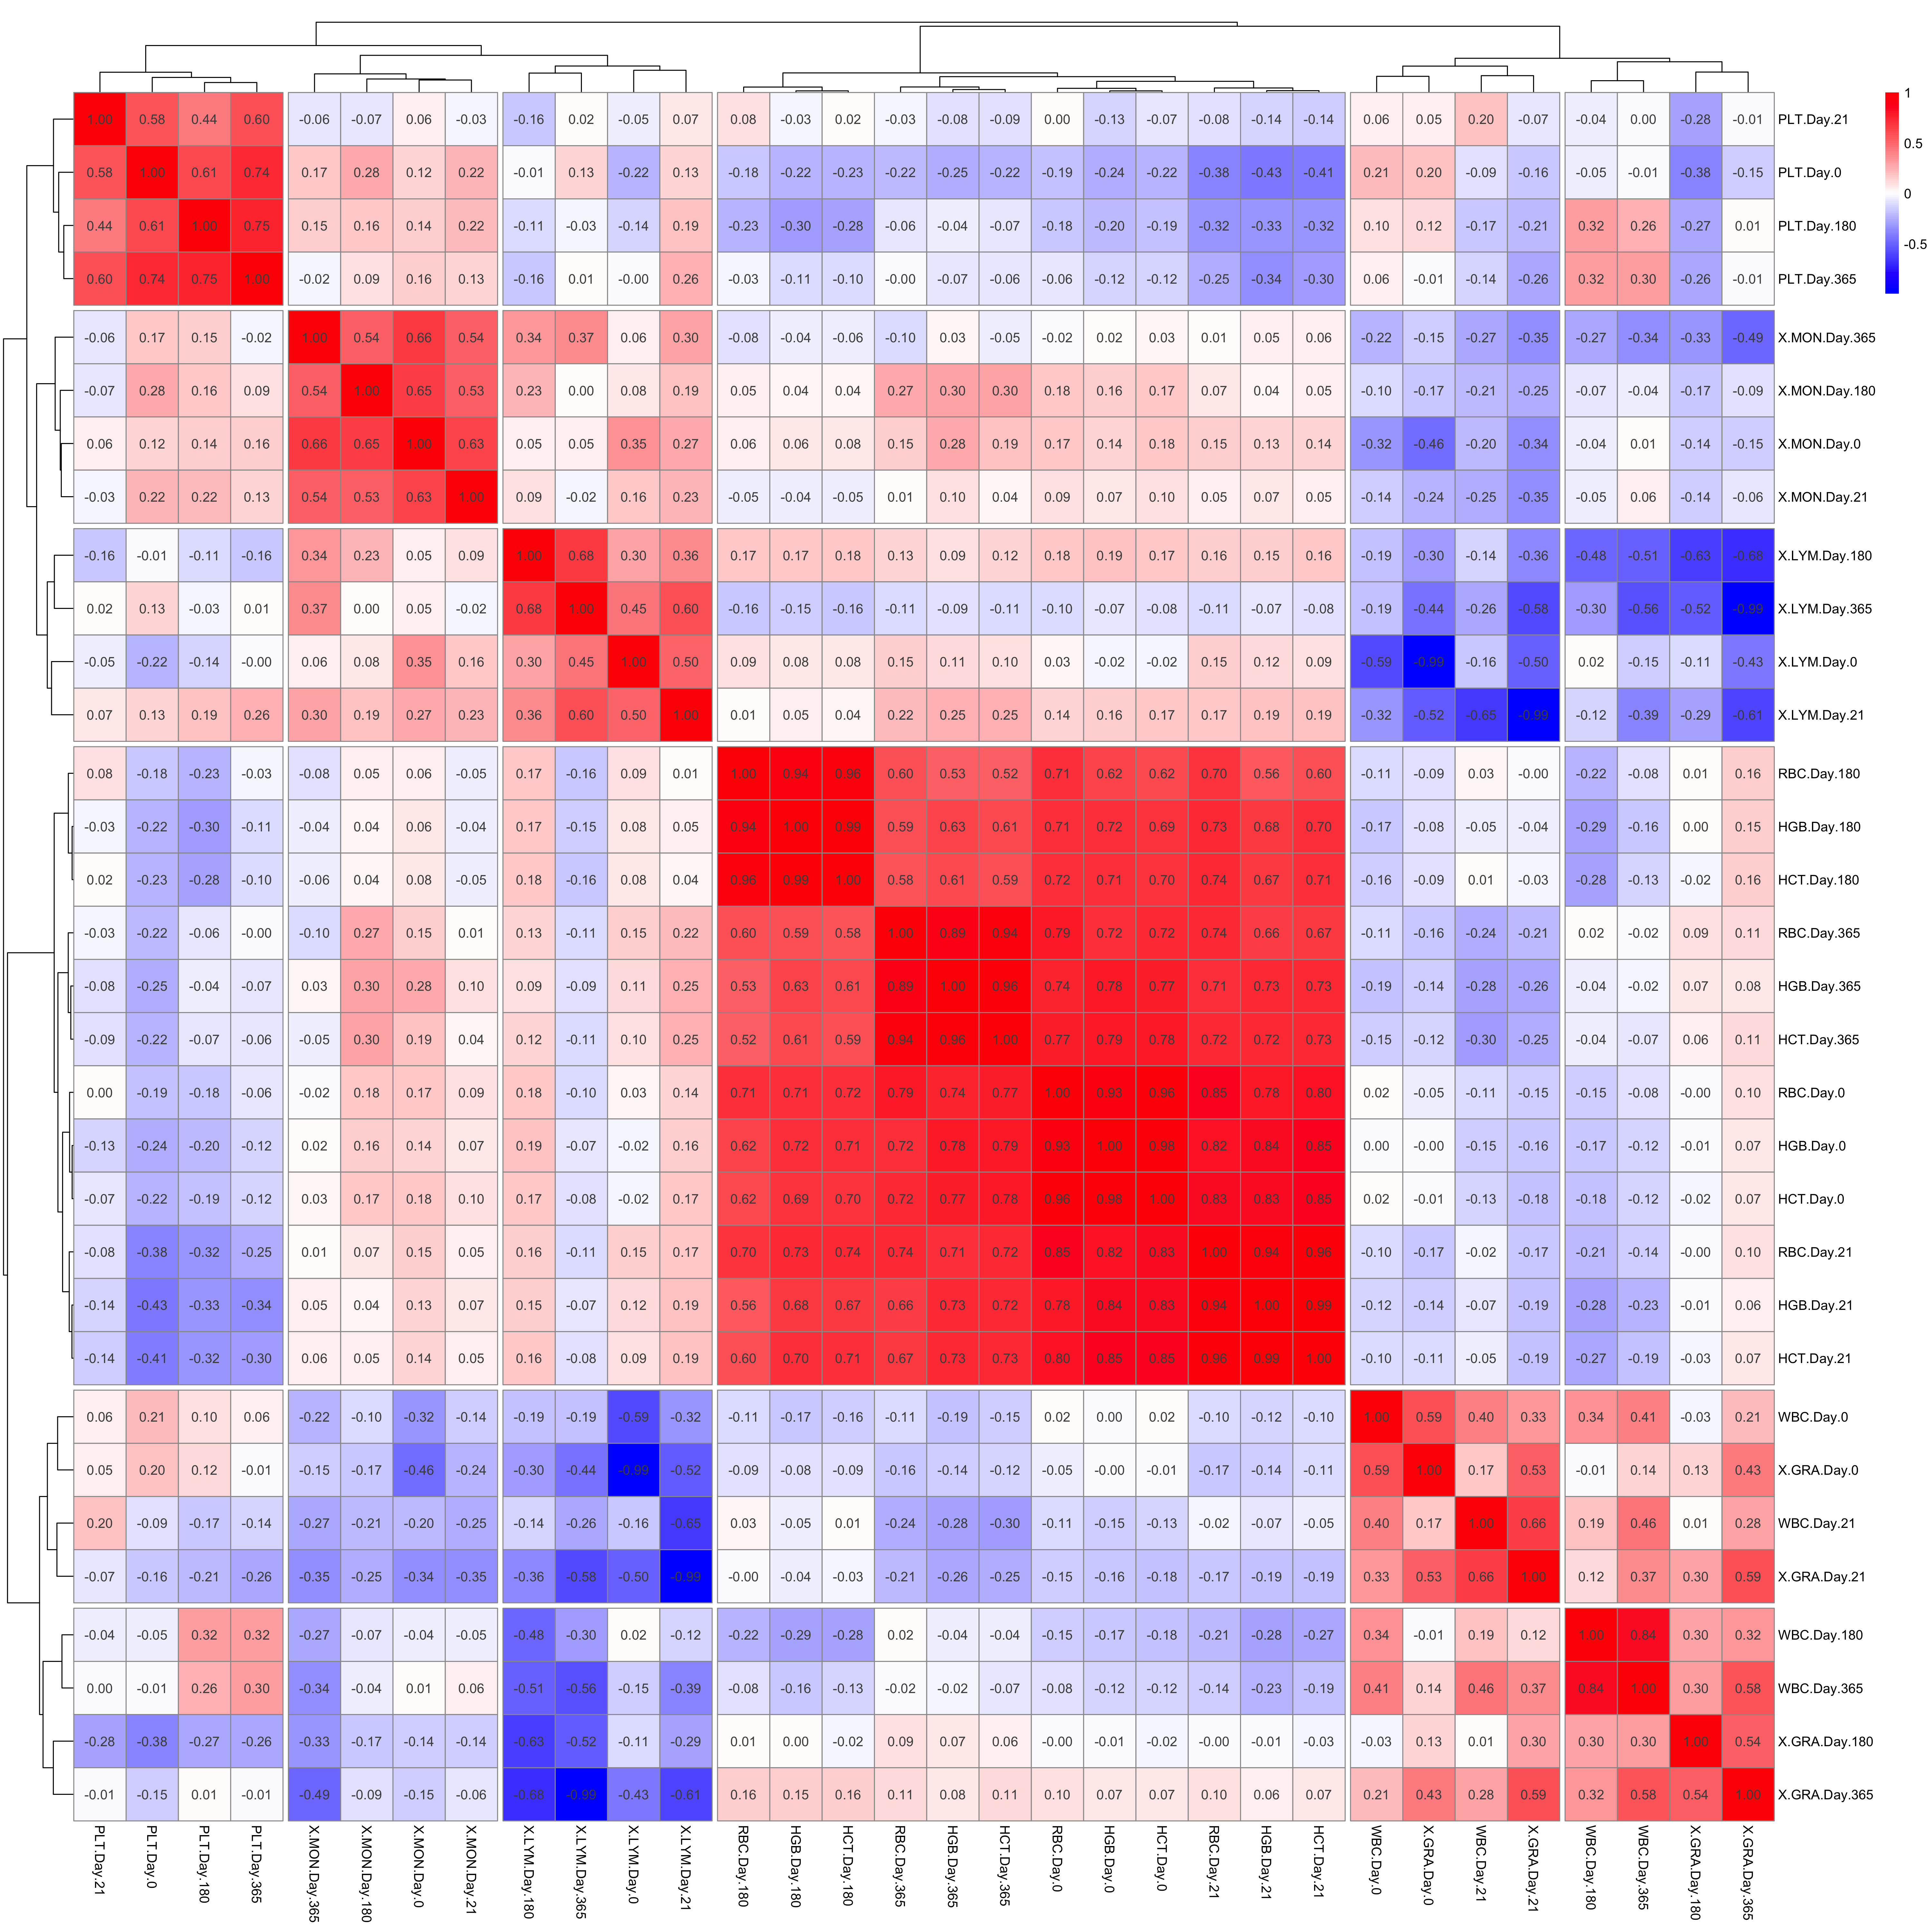
\includegraphics[width=0.8\textwidth]{images/Cytometry_euclidean_distance.png}
  \caption[cytometry data correlations]{Correlation heatmap of the cytometry data using hierarchical clustering.}
  \label{fig:cytometry_heatmap}
\end{figure}
\noindent
At Day~0, the heatmap reveals high correlation coefficients (e.g., 0.89--0.99) among \acrshort{rbc}, \acrshort{hgb}, and \acrshort{hct}, and similar correlation patterns emerge at Day~0, Day~21, Day~180, and Day~365, reinforcing their consistent co-variation over time. Even when only Day~0 is considered. (For the corresponding dendrogram, refer to Figure~\ref{fig:Cytometry_features_clustering_cut_colors} in Appendix~\ref{appendix:cytometry_features_clusterings}).
\begin{table}[h!]
    \centering
    \begin{tabular}{ll}
        \textbf{Cluster 1:} &  \acrshort{rbc}, \acrshort{hgb}, and \acrshort{hct}
    \end{tabular}
    \caption{Cytometry Clusters}
    \label{tab:cytometry_clusters}
\end{table}



\subsection{\acrshort{rna} Data}
\begin{figure}[H]
  \centering
  \includegraphics[width=0.8\textwidth]{images/circos_RNA_only.png}
 \caption[\acrshort{rna} data correlations circular]{Circular correlation plot of the \acrshort{rna} data. Each feature is represented along the outer edge. Points within the tracks represent the mean expression level for each feature across different response groups. Colored lines indicate correlations between features (blue for positive correlations, red for negative correlations). The dense network of lines highlights the complexity of the dataset and the difficulty in visually identifying specific patterns or clusters.}
  \label{fig:rna_circos}
\end{figure}

The \acrshort{rna} dataset presented a greater challenge for correlation analysis due to the high dimensionality, with a total of 382 features. To explore potential relationships within this data, various visualization techniques where employed, including the circular plot shown above.\\
\\
 Although the plot provides a comprehensive overview of all possible correlations, the dense web of lines makes it difficult to discern specific patterns or clusters visually. However, the primary advantage of this visualization is that it allows for the identification of broad trends and the detection of features that may be particularly well-connected or influential.

\begin{figure}[H]
  \centering
  \includegraphics[width=0.8\textwidth]{images/RNA_euclidean_distance.png}
  \caption[\acrshort{rna} data correlations]{Correlation heatmap of the \acrshort{rna} data using hierarchical clustering.}
  \label{fig:RNA_heatmap}
\end{figure}

\noindent
The same heatmap visualization technique (as used for Figures~\ref{fig:cytokine_heatmap} and~\ref{fig:cytometry_heatmap}) was applied to the \acrshort{rna} dataset, using a total of 36 cuts to correspond to the 36 different \acrshort{rna} modules identified through hierarchical clustering. Selecting 36 cuts was challenging, but this number provided a reasonable balance between capturing distinct clusters and maintaining interpretability. The heatmap effectively highlights clear blocks of positively (red) and negatively (blue) correlated features. The precise cut point within the hierarchical tree that resulted in these 36 modules is visually represented in Figure~\ref{fig:RNA_features_clustering_cut_colors} (Appendix~\ref{appendix:rna_features_clusterings}). For further details of the features comprising each of the 36 identified RNA modules, please refer to Table~\ref{tab:clustered_terms_RNA}, located in the Supplemental Material.
%%%%%%%%%%%%%%%%%%%%%%%%%%%%%%%%%%%%%%%%%%%%%%%%%%%%%%%%%%%%%%%%%%%%%%%%%%%%%%%%%%%%%%%%%%%%%%%%%%%%%%%%%%%%%%%%%%%%%%%%%%%%%%%%%%%%%%%%%%%%%%%%%





\chapter{Methodology: Modeling and Feature Selection for Measles}
\label{chap:methodology}
%%%%%%%%%%%%%%%%%%%%%%%%%%%%%%%%%%%%%%%%%%%%%%%%%%%%%%%%%%%%%%%%%%%%%%%%%%%%%%%%%%%%%%%%%%%%%%%%%%%%%%%%%%%%%%%%%%%%%%%%%%%%%%%%%%%%%%%%%%%%%%%%%
%\todo{Explain your pipeline for exploratory analysis, model building, and selection of stable predictive features, highlighting the specific challenges and how they were overcome.}
\section{Consensus Model Approach}
\label{sec:consensus_model_approach}
\noindent
In the initial phase of the modeling process, this study opted for a consensus model approach to leverage the complementary strengths of multiple predictive models. This technique involves training several distinct models independently on the different datasets and then concatenating their responses to form a unified prediction. The reason behind this approach is that different models may capture unique aspects of the data or be sensitive to different feature sets, thus enhancing the overall robustness and generalizability of the predictions.\\
\\
It is noteworthy that while many conventional consensus or ensemble learning strategies achieve diversity by applying different model algorithms or parameterizations primarily to a single dataset or variations thereof \cite{Rokach2010}, the approach adopted in this thesis introduces diversity fundamentally at the data level. Here, distinct modeling pipelines, each including internal model evaluation and selection, are applied independently to multiple, heterogeneous datasets (cytokines, cytometry, clonal breadth, clonal depth, \acrshort{rna} data), each representing a different biological viewpoint. Only after each pipeline generates its best prediction on the validation set are these modality-specific test set outputs aggregated.\\
\\
By combining model outputs, the consensus approach aims to mitigate individual model biases and reduce the risk of overfitting, particularly given the high-dimensional nature and small size of the dataset. However, the complexity introduced by this approach requires careful consideration of how model outputs are integrated and evaluated.

\begin{figure}[H]
  \centering
  \hspace*{-0.9cm}
  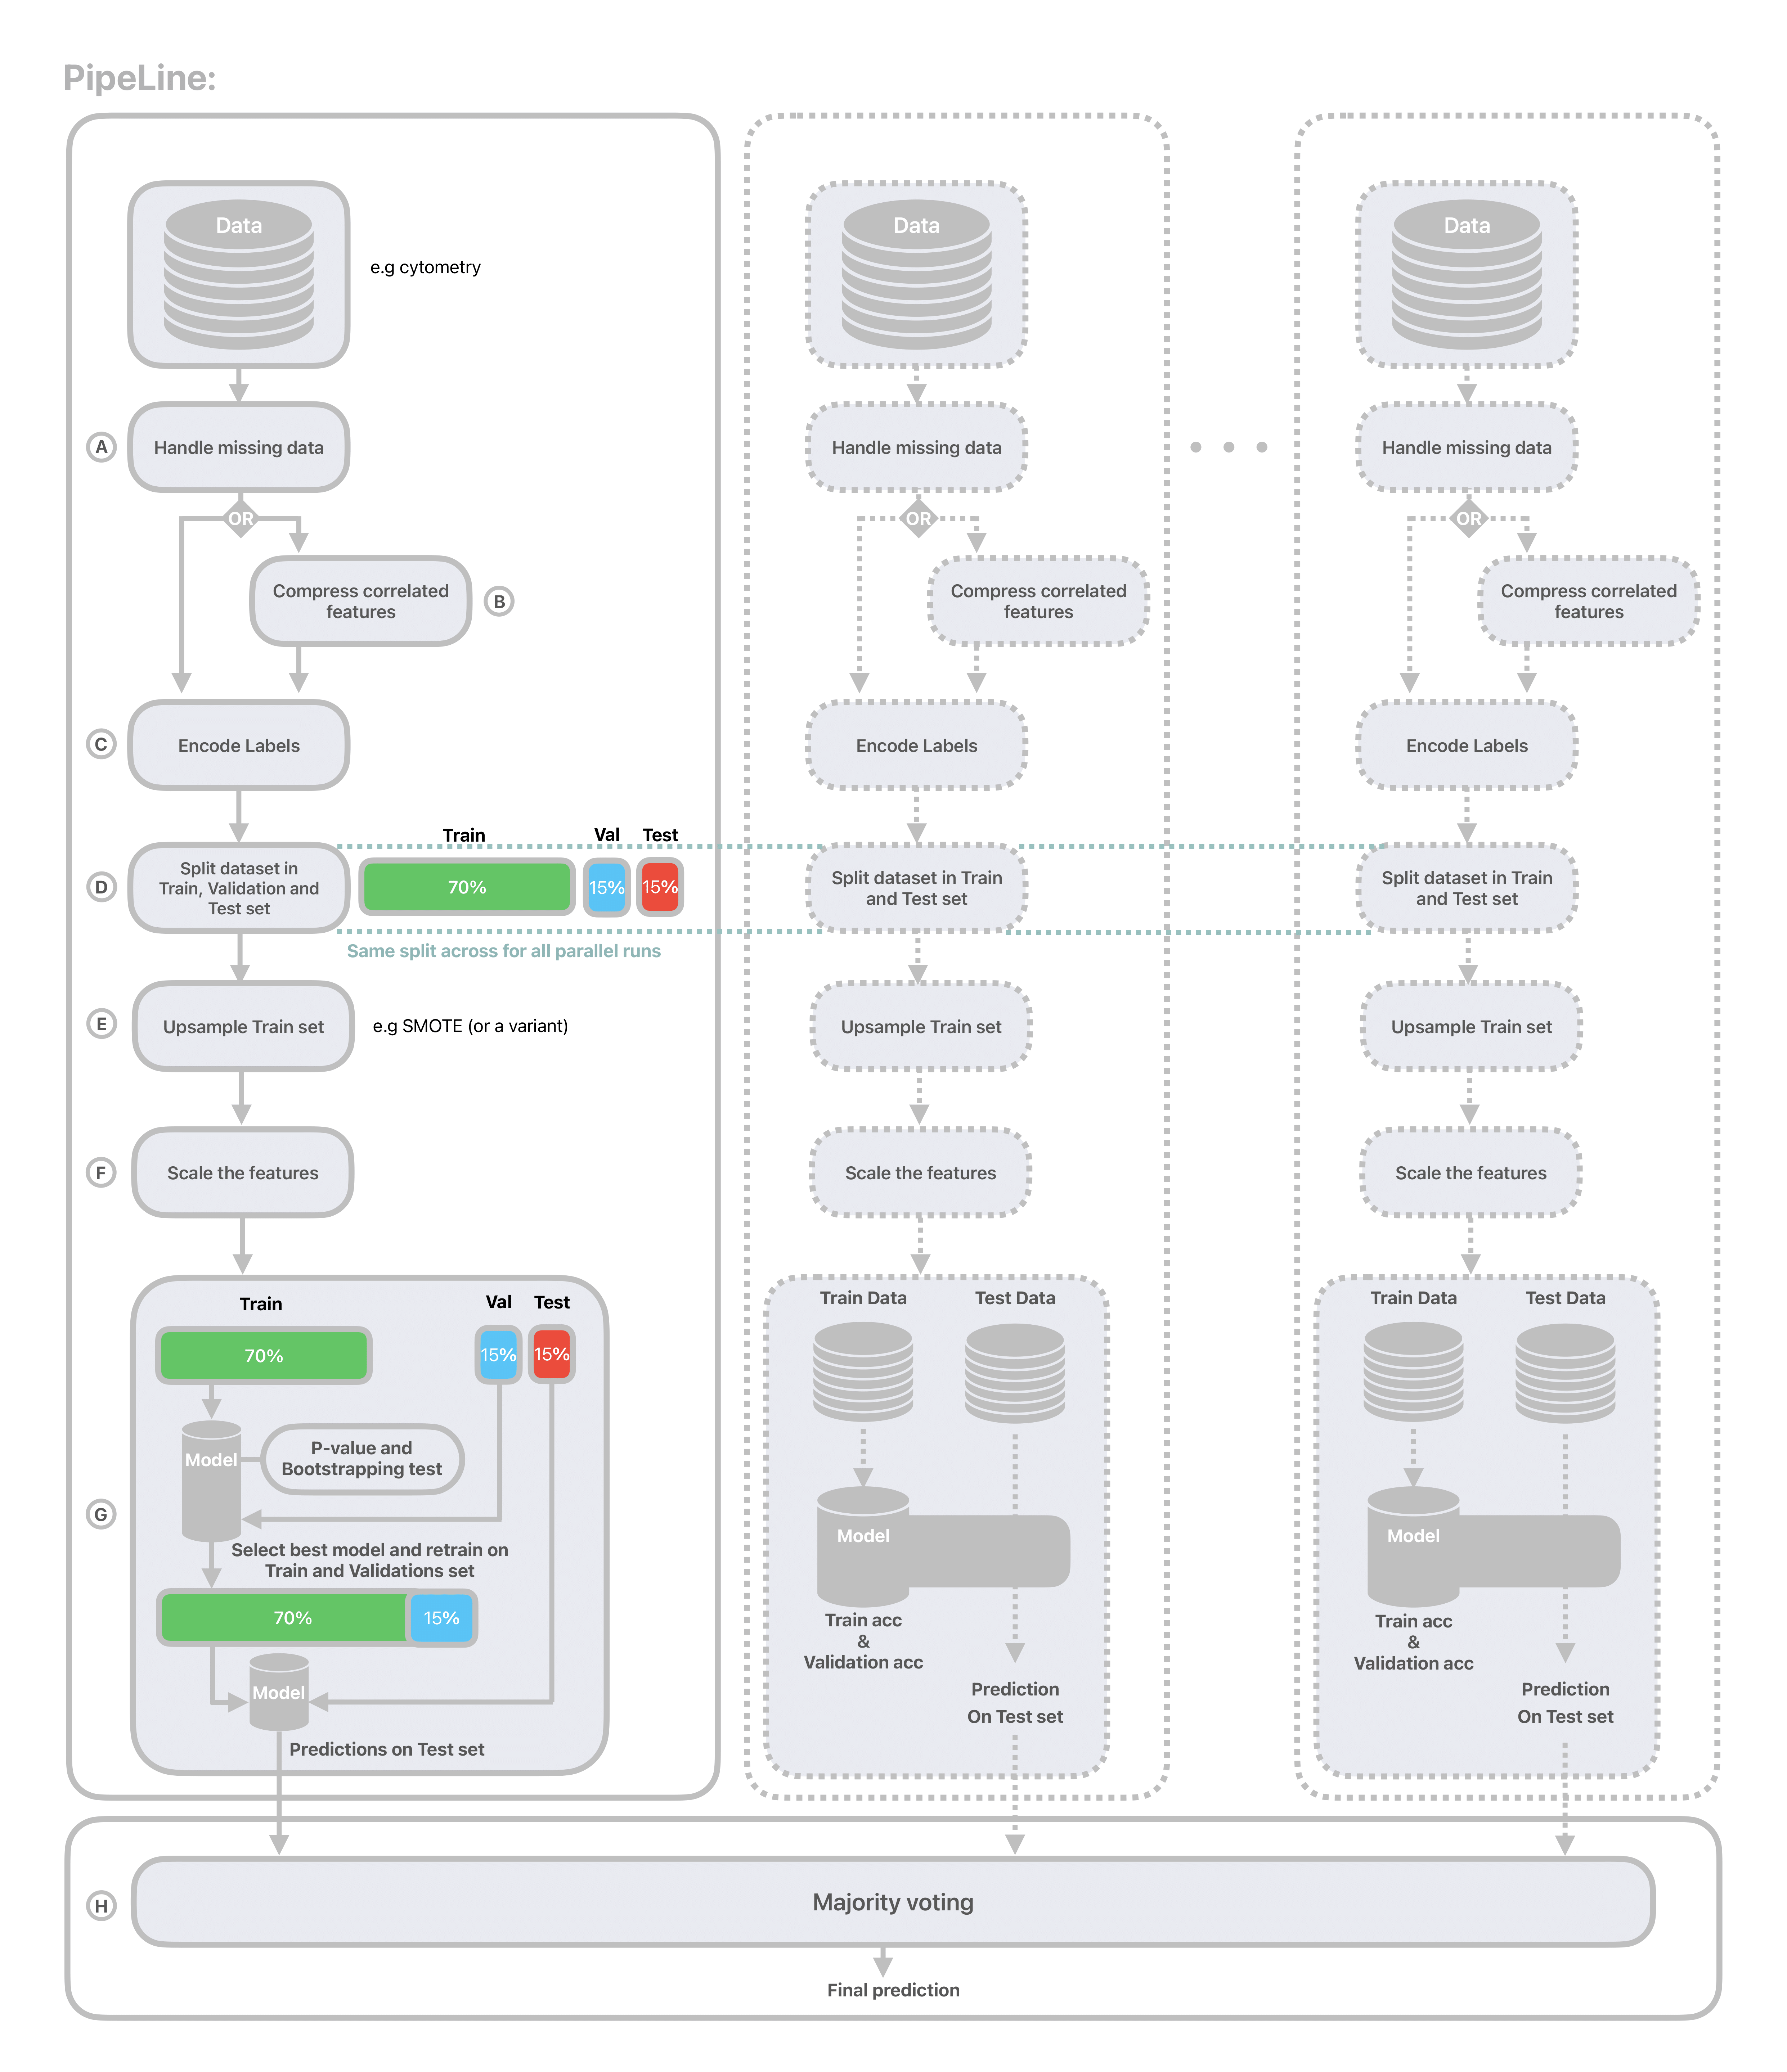
\includegraphics[width=1.1\textwidth]{images/Pipeline-1.png}
  \caption[Consensus model pipeline diagram]{The diagram illustrates the multi-model pipeline used for prediction. Each individual model follows a standardized preprocessing workflow: data loading, preprocessing (A: Missing data handling, B: Feature compression, C: Label encoding, F: Feature scaling), data splitting (D), upsampling the training set (e.g., using random upsampling or \acrshort{smote}) (E). The trained models then produce predictions, which are evaluated based on training, validation and testing accuracy. Additional validation is performed using p-value assessment and bootstrapping to ensure robustness (G). The final prediction is obtained through majority voting, aggregating predictions from all models to produce a consensus output (H).}
  \label{fig:pipeline-1}
\end{figure}

\subsection{Pipeline Structure for Heterogeneous Datasets}
\label{subsec:pipeline_structure_for_heterogeneous_datasets}
\noindent
This section details the structure applied within the consensus modeling framework. Specifically, five parallel pipelines were executed, each dedicated to one of the following distinct data types:
Cytokine measurements, Cytometry data, T-cell clonal breadth metrics, T-cell clonal depth metrics and \acrshort{rna} sequencing data.\\
\\
Although each pipeline starts with different data to capture unique biological insights, maintaining consistency across them is essential. Therefore, the same standardized workflow is applied to all five pipelines after loading their specific data. Using this uniform process ensures each distinct data type is handled the same before the final predictions are combined. As illustrated in Figure~\ref{fig:pipeline-1}, the standardized workflow applied to each dataset involves the following sequential steps:

\subsubsection*{Missing data handling \hyperref[fig:pipeline-1]{(A)}}
The initial step in the preprocessing pipeline involved a systematic check for missing values within the feature columns of each dataset. This is a standard procedure, as many machine learning algorithms require complete data matrices for training and prediction. Upon inspection of the datasets used in this study, no missing values were found within the feature columns relevant to the modeling process. Therefore, this step primarily served as a data integrity verification, and no imputation or sample removal actions due to missing feature values were necessary. (Handling of entire missing patient records for certain datasets was addressed during the data splitting phase as described in \textbf{{Split dataset(D)}}).

\subsubsection*{Compress correlated features \hyperref[fig:pipeline-1]{(B)}}
This step focused on addressing highly correlated features within each dataset, based on the findings presented in Section~\ref{sec:correlation_analysis_within_individual_datasets}. To mitigate potential multicollinearity issues, these identified features were subsequently compressed into a single dimension using \gls{pca}, resulting in one principal component that represented them in the 'compressed' feature set.\\
\\
To investigate whether feature compression impacted the final consensus model's performance, the modeling pipeline following this step was executed using two parallel approaches for each dataset. One approach utilized the original, full set of features, while the other used the reduced feature set. While addressing correlated features can potentially reduce redundancy and improve model stability, the main purpose of this parallel analysis was to empirically determine if this compression step offered a measurable advantage to the predictive accuracy of the overall consensus model for each specific data type.

\subsubsection*{Labels encoding \hyperref[fig:pipeline-1]{(C)}}
As machine learning algorithms typically require numerical inputs, the categorical target variable was converted into a numerical format in this step. This encoding simply assigned a unique integer (e.g., 0 and 1) to each response class.

\subsubsection*{Split dataset \hyperref[fig:pipeline-1]{(D)}}
To properly evaluate model performance and ensure generalization to new data, the dataset was partitioned into three independent subsets: a training set, a validation set, and a test set.\\
\\
The partitioning followed a 70\% / 15\% / 15\% ratio, allocating the data as follows:
\begin{itemize}
    \item \textbf{Training Set (70\%):} This largest subset was used solely for training the models. The algorithms learn patterns, relationships, and parameters from this data.
    \item \textbf{Validation Set (15\%):} This independent subset was crucial during the model development phase, specifically for selecting the optimal combination of model algorithm and data preprocessing choices. Since multiple distinct model types were evaluated in parallel across the pipelines, and different up-sampling techniques were considered (detailed in the next step), this validation set was used to compare their performance. The combination of model algorithm and up-sampling method yielding the best results on the validation set was selected for final evaluation. Performing the model and up-sampling selection using the validation set is critical to ensure that the test set remains completely untouched and unseen, thereby preserving its integrity for the final, unbiased assessment of generalization performance.
    \item \textbf{Test Set (15\%):} This subset was strictly held out until all model development and selection were finalized based on the training and validation sets. It was used only once at the very end to provide a final, unbiased estimate of how the chosen model configuration is expected to perform on new, unseen data.
\end{itemize}
\noindent
The datasets presented a challenge in terms of sample size consistency: cytokine, cytometry, and \acrshort{rna} data were available for all 40 patients, whereas clonal breadth and depth data were limited to 27 patients. Despite this discrepancy, evaluating the performance of each pipeline and, critically, aggregating their predictions for the final consensus model requires that all analyses utilize the exact same held-out test set. Maintaining this test set consistency across all data modalities was therefore essential for the validity of the study's comparative evaluations and the subsequent consensus aggregation via majority voting.

\begin{figure}[H]
  \centering
  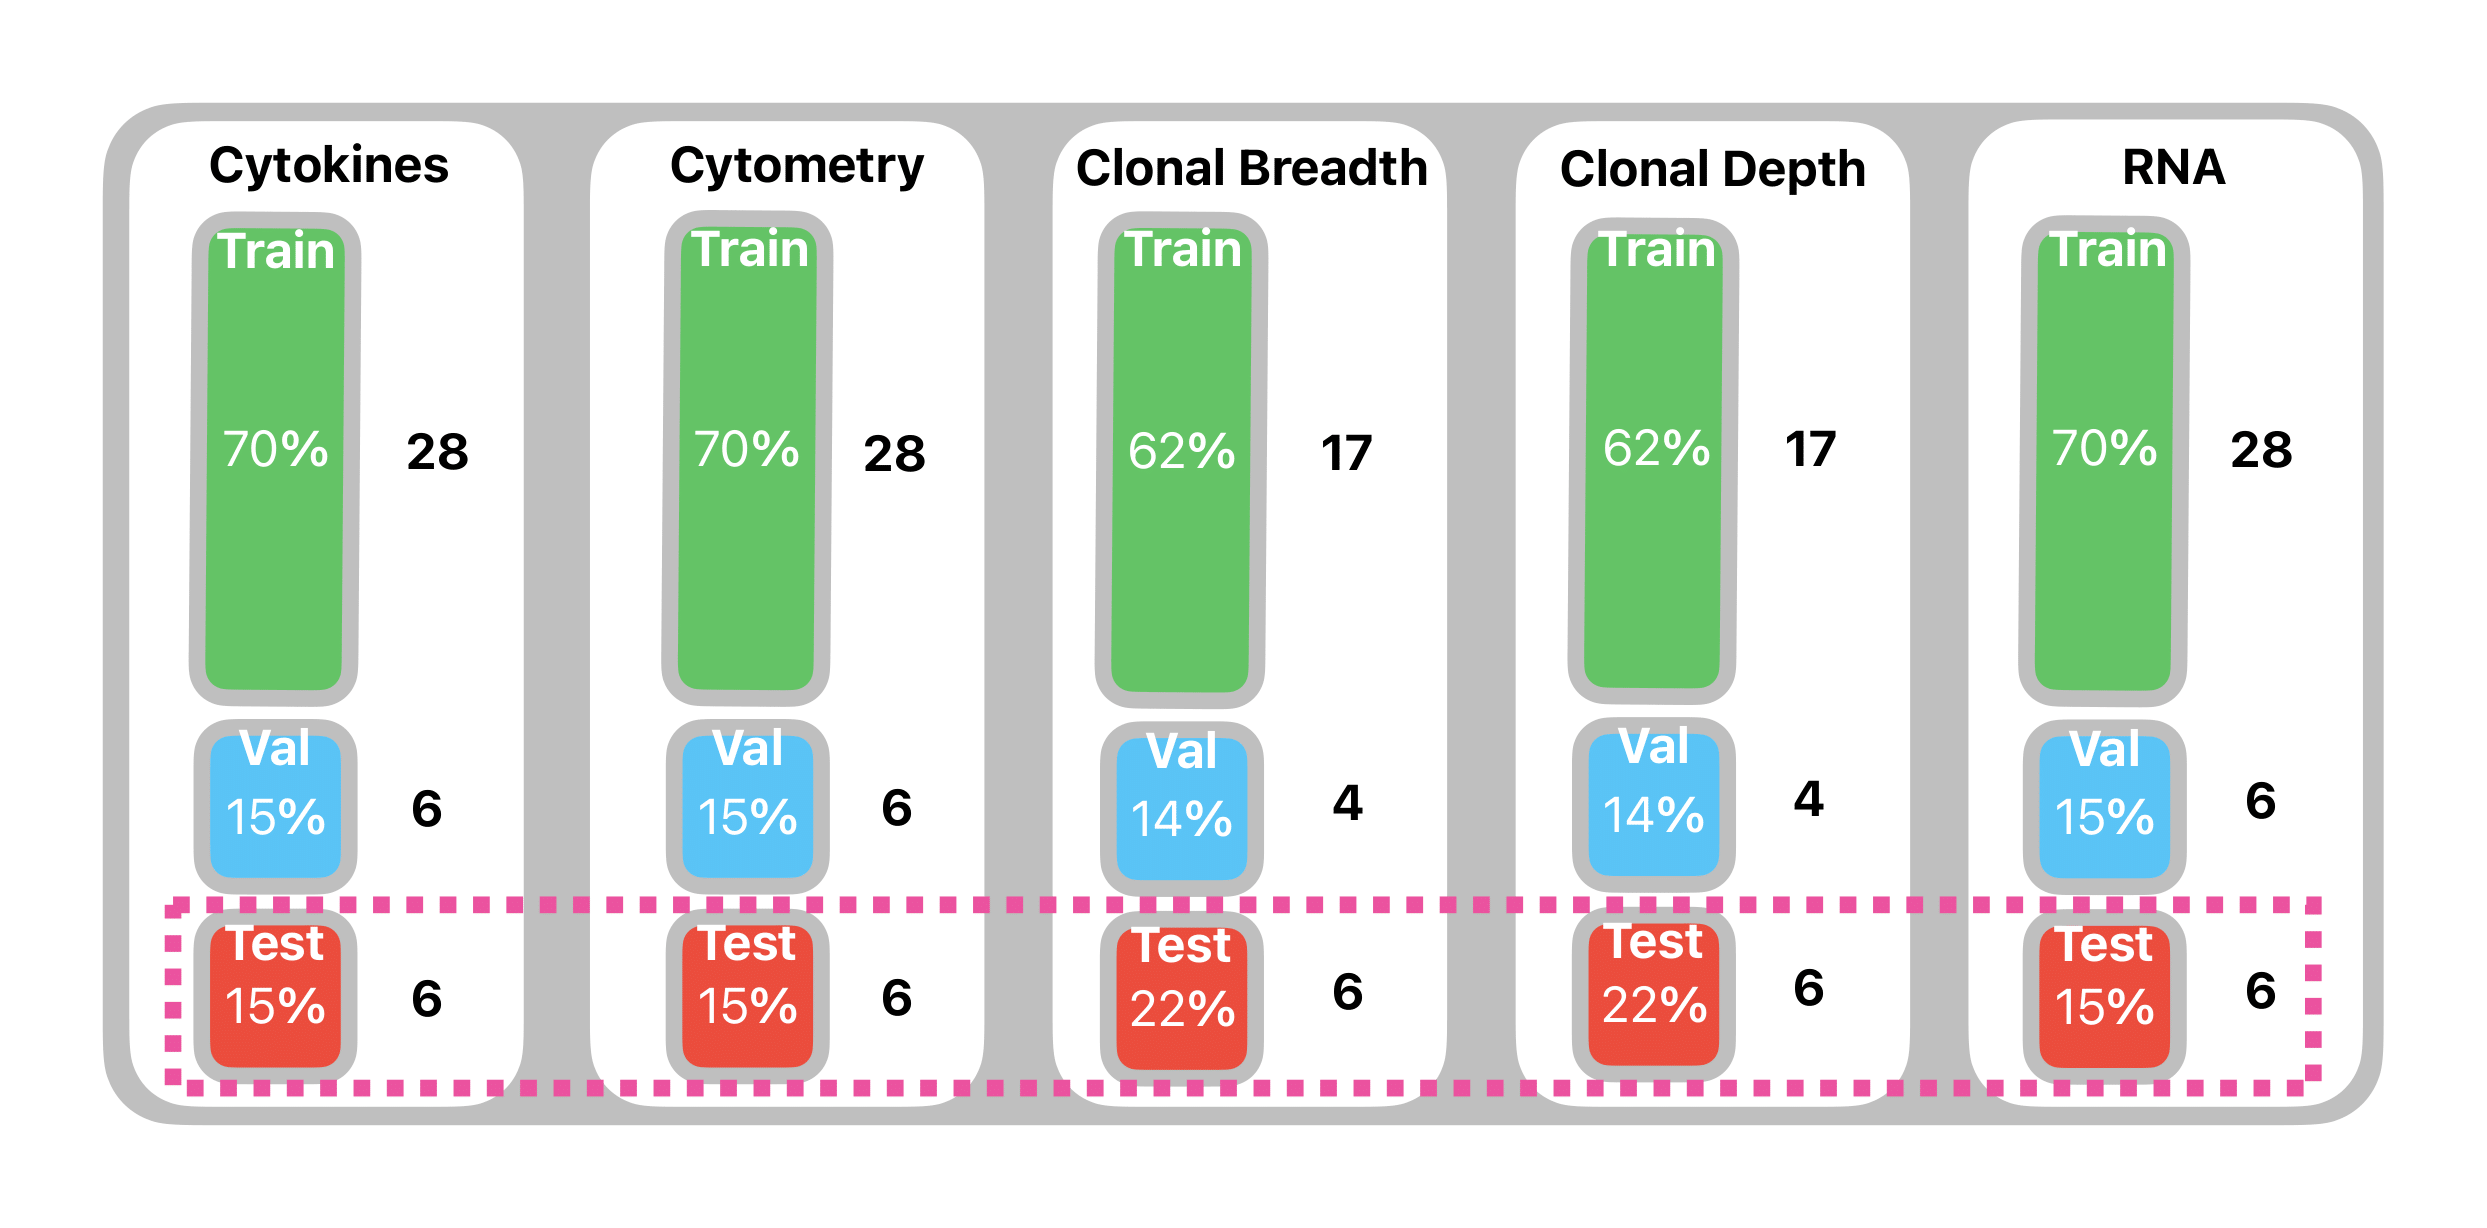
\includegraphics[width=0.8\textwidth]{images/split-1.png}
    \caption[Data splits per modality]{Visual summary of the Train/Validation/Test set splits applied to each data modality, showing sample counts and highlighting the consistent test set size (N=6).}
  \label{fig:split_data}
\end{figure}
\noindent
To achieve this, a global data partitioning strategy was defined based on the complete 40-patient cohort. A standard 70\% / 15\% / 15\% ratio was applied to this full cohort to designate specific individuals for the training (n=28), validation (n=6), and test (n=6) sets.\\
\\
This partitioning was applied directly to the complete datasets (cytokine, cytometry, \acrshort{rna}), resulting in the target split of 28/6/6. For the clonal depth and breadth datasets (N = 27), which represented subsets of the full cohort, a specific procedure ensured the consistency of the test set: the same 6 individuals designated globally for the test set were identified within the 27 available samples and assigned as the test set for these modalities. The remaining 21 samples specific to these datasets were then subsequently divided into training and validation sets, using an approximate 80\%/20\% split of this remainder, which resulted in 17 training samples and 4 validation samples for the clonal breadth and depth pipelines as can be seen in Figure~\ref{fig:split_data}.\\
\\
While this approach successfully maintained the crucial consistency of the test set across all analyses, it necessarily resulted in different effective sizes and ratios for the training and validation partitions in the clonal datasets (approx. 63\% Train / 15\% Val / 22\% Test) compared to the others (70\% Train / 15\% Val / 15\% Test). This variation was deemed an acceptable trade-off to preserve the integrity of the final, comparative evaluation on a common test cohort.


\subsubsection*{Up-sample Train set \hyperref[fig:pipeline-1]{(E)}}
\label{subsubsec:up-sample_train_set}
A common challenge in biological datasets is class imbalance, where one response class (in this case, responders) may be significantly less prevalent than the other within the training data. This may cause the model to favor the majority class during training. To counteract this and evaluate different mitigation approaches, three distinct strategies for handling class imbalance were applied exclusively to the training sets:

\begin{enumerate}
    \item \textbf{No Resampling with Class Weighting:} In this strategy, the inherent distribution of labels  was not modified. Instead, imbalance was addressed algorithmically during model training by assigning higher weights to the minority class samples. This typically adjusts the model's loss function, making errors on minority class examples more costly and forcing the model to pay more attention to them.
    \item \textbf{\gls{ros}:} This method directly modifies the training set by increasing the representation of the minority class. It works by randomly selecting and duplicating existing samples from the minority class until an equal number of samples per class is achieved.
    \item \textbf{\acrfull{smote}:} Generates new, synthetic minority class samples through feature space interpolation, as detailed further below and illustrated in Figure~\ref{fig:SMOTE_explained}.
\end{enumerate}

\begin{figure}[htbp]
    \centering
    % Verify path is correct
    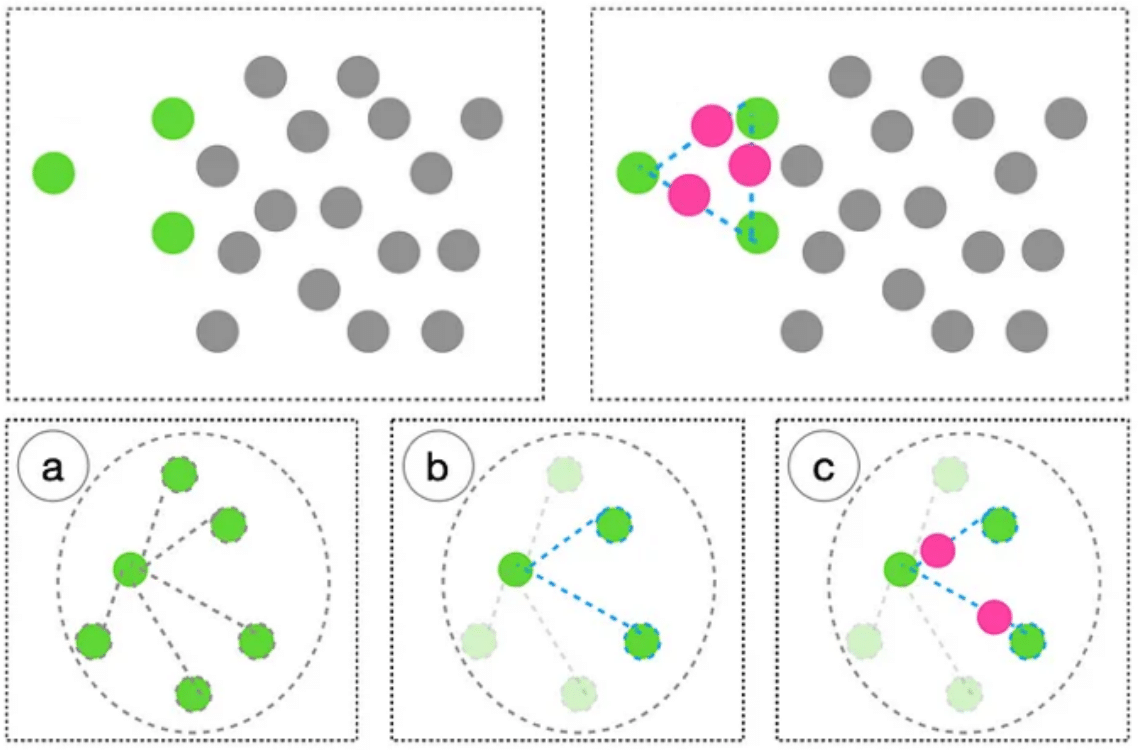
\includegraphics[width=0.8\textwidth]{images/SMOTE-explained.png}
    \caption[Illustration of the \gls{smote} mechanism]{Illustration of the \gls{smote} mechanism. Top left: Initial imbalanced data distribution (minority in green, majority in gray). Top right: Generation of synthetic samples (pink) along lines connecting a minority instance to its nearest minority neighbors. Bottom row: Detailed steps showing (a) identification of k-nearest minority neighbors (here k=5), (b) selection of neighbors for synthesis, and (c) creation of synthetic samples (pink) along the vectors to selected neighbors. Figure based on Figures 1 and 2 presented in \cite{Truong2022SMOTEVariants}.}
    \label{fig:SMOTE_explained} % Unique label
\end{figure}

\begin{figure}[htbp]
    \centering
    % Verify path is correct
    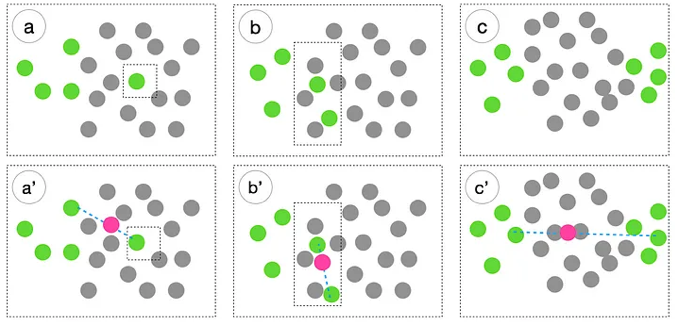
\includegraphics[width=0.8\textwidth]{images/SMOTE-weaknesses.png}
    \caption[Illustration of \gls{smote} weaknesses]{Conceptual illustration of potential weaknesses associated with \gls{smote}. The bottom row (a', b', c') depicts synthetic sample generation (pink) relative to regions shown in the top row (a, b, c). Potential issues illustrated include: (a/a') Generation influenced by potential noise or outliers (isolated minority sample). (b/b') Synthetic samples potentially overlapping with dense majority class regions due to disregard for majority sample proximity. (c/c') Generation possibly bridging distinct minority clusters, which could ignore underlying data structure or cause overgeneralization. Figure adapted from Figure 4 presented in \cite{Truong2022SMOTEVariants}.}
    \label{fig:SMOTE_weaknesses} % Unique label
\end{figure}

\noindent
\gls{smote} \cite{Chawla2002SMOTE}, visually explained in Figure~\ref{fig:SMOTE_explained} operates in the feature space, utilizing the relative positions of minority instances to generate new samples. It selects a minority instance, finds its k-nearest minority class neighbors, and creates new samples along the line segments joining the instance to some of these neighbors. This method can potentially create a more diverse minority representation and smoother decision boundaries.\\
\\
However, \gls{smote} also has known limitations (illustrated in Figure~\ref{fig:SMOTE_weaknesses}), as discussed in literature \cite{Truong2022SMOTEVariants}. Potential drawbacks include overgeneralization (creating samples that blur class distinctions or ignore sub-clusters), amplification of noise if based on outlier samples, and possible generation of samples too close to or overlapping with the majority class, as the original algorithm doesn't explicitly consider majority proximity. Despite these points, \gls{smote} was included for comparison as a prominent synthetic data generation technique.\\
\\
The relative effectiveness of these three imbalance-handling strategies (Class Weighting, \gls{ros}, \gls{smote}) was assessed empirically for each model pipeline. As established during data splitting, the performance metrics achieved on the 15\% validation set were used to select the optimal strategy for each model before final assessment on the test set. It is crucial to mention again that these imbalance adjustments were applied strictly to the training data to maintain the integrity of the validation and test sets.

\subsubsection*{Scale the features \hyperref[fig:pipeline-1]{(F)}}
Feature scaling was applied to standardize the range of the input features. This ensures that features with larger values do not disproportionately influence distance-based or gradient-based machine learning algorithms. Using scikit-learn's \texttt{StandardScaler}, the features in the training set were scaled to have zero mean and unit variance. The parameters learned from the training set were then used to transform the validation and test sets consistently, preventing data leakage.


\subsubsection*{Train the models \hyperref[fig:pipeline-1]{(G)}}
\noindent
Following the comprehensive preprocessing stages (A-F) designed to prepare each dataset modality, the pipeline proceeds to the core modeling phase. The objective here is not necessarily to find a single universally best model through extensive tuning, but rather to train, rigorously evaluate, and select the most suitable baseline classification algorithm for each distinct pipeline configuration. That is, for each combination of initial dataset (e.g., cytokines, cytometry) and class imbalance handling strategy (weighting, \gls{ros}, or \gls{smote}). Feature compression was considered in a parallel run.\\
\\
A suite of five standard, well-established classification algorithms were employed as candidates within each pipeline shown in Table~\ref{tab:ml_models}. These models were generally used with default hyperparameters to provide a robust baseline comparison. If the class weighting strategy was selected in the preceding step, balanced class weights were incorporated into the algorithms during training.\\
\begin{table}[h!]
    \centering
    \scalebox{0.8}{%
    \begin{tabular}{lllll}
        \toprule
        Model & Configurations & & \\
        \midrule
        Random Forest (RF) & \textit{Default scikit-learn parameters}, & \texttt{random\_state=42}, & \\
        Logistic Regression (LogReg) & \textit{Default scikit-learn parameters}, & \texttt{random\_state=42}, & \texttt{max\_iter=1000} \\
        Support Vector Machine (SVM) & \textit{Default scikit-learn parameters}, & \texttt{random\_state=42}, & \texttt{probability=True} \\
        Decision Tree (DT) & \textit{Default scikit-learn parameters}, &  \texttt{random\_state=42}, & \\
        Gaussian Naive Bayes (NB) & \textit{Default scikit-learn parameters},  & & \\
        \bottomrule
    \end{tabular}}
    \caption[Machine Learning Models Used]{Machine Learning Models Used and their Configurations}
    \label{tab:ml_models}
\end{table}
\\
\noindent
The process of identifying the best model for each configuration began with training each candidate algorithm on its corresponding partition of training data (70\%). Following this initial training, the intrinsic stability and statistical significance of the model were rigorously assessed using the training data itself. Performance stability was evaluated through repeated 5-fold stratified cross-validation (n = 1000 repetitions), a procedure illustrated in Figure~\ref{fig:Bootstrapping-1}. This yielded a mean performance score and confidence intervals, providing insight into the robustness of the model's performance against variations in the training data splits. The statistical significance of this performance, relative to chance, was then determined using permutation tests (n = 1000 permutations), as shown in Figure~\ref{fig:P-value_test-1}. This test resulted in a p-value, quantifying the likelihood that the observed cross-validation performance could have arisen simply due to random chance.\\
\\
Although these initial evaluations provided valuable insights into model characteristics on the training distribution, the definitive selection of the optimal model for the specific pipeline was driven by performance on the independent 15\% validation set. Each trained candidate model generated predictions for the validation set samples, and a composite score (derived from the weighted F1-score and balanced accuracy) was calculated. The algorithm that achieved the highest composite score on the validation set was selected as the preferred model for that configuration. In the event of ties in the composite score (partly due to the very low sample size), the mean cross-validation score and subsequently the permutation test p-value (both derived from the training set evaluations) served as hierarchical tie-breakers.\\
\\
Once the best model algorithm was identified for a given configuration (e.g., SVM selected for Cytokine data processed with \gls{smote} and \gls{pca}), it underwent a final retraining step. This involved re-fitting the selected model architecture using a combination of the 70\% training partition and the 15\% validation partition. By retraining on this larger (85\%) dataset, the final model could potentially learn a more refined parameterization before deployment on unseen data. Finally, this fully trained model was applied to the completely untouched 15\% test set to generate the ultimate predictions for that specific pipeline configuration. These test set predictions were used in the final step to combine results from all the different model pipelines.\\
\\
This entire process (preprocessing, training, evaluation, selection, retraining, prediction) was executed in parallel for all configurations being tested (e.g., for cytokines with weighting, cytokines with \gls{ros}, cytokines with \gls{smote}, potentially repeated with/without \gls{pca}, and similarly for cytometry, clonal breadth, etc.). This resulted in multiple sets of predictions for the same test set, each derived from the best model identified for a specific pathway. These multiple prediction sets then serve as the input for the final consensus aggregation step, described next.

\subsubsection*{Consensus model\hyperref[fig:pipeline-1]{(H)}}
Finally, to produce the single output prediction of the overall consensus model, the predictions generated for the test set by each of the parallel pipeline configurations were aggregated. This aggregation was performed using "Majority Voting". For every sample in the test set, the class label predicted most frequently across all contributing pipeline models was selected as the final consensus prediction.

\begin{figure}[H]
  \centering
  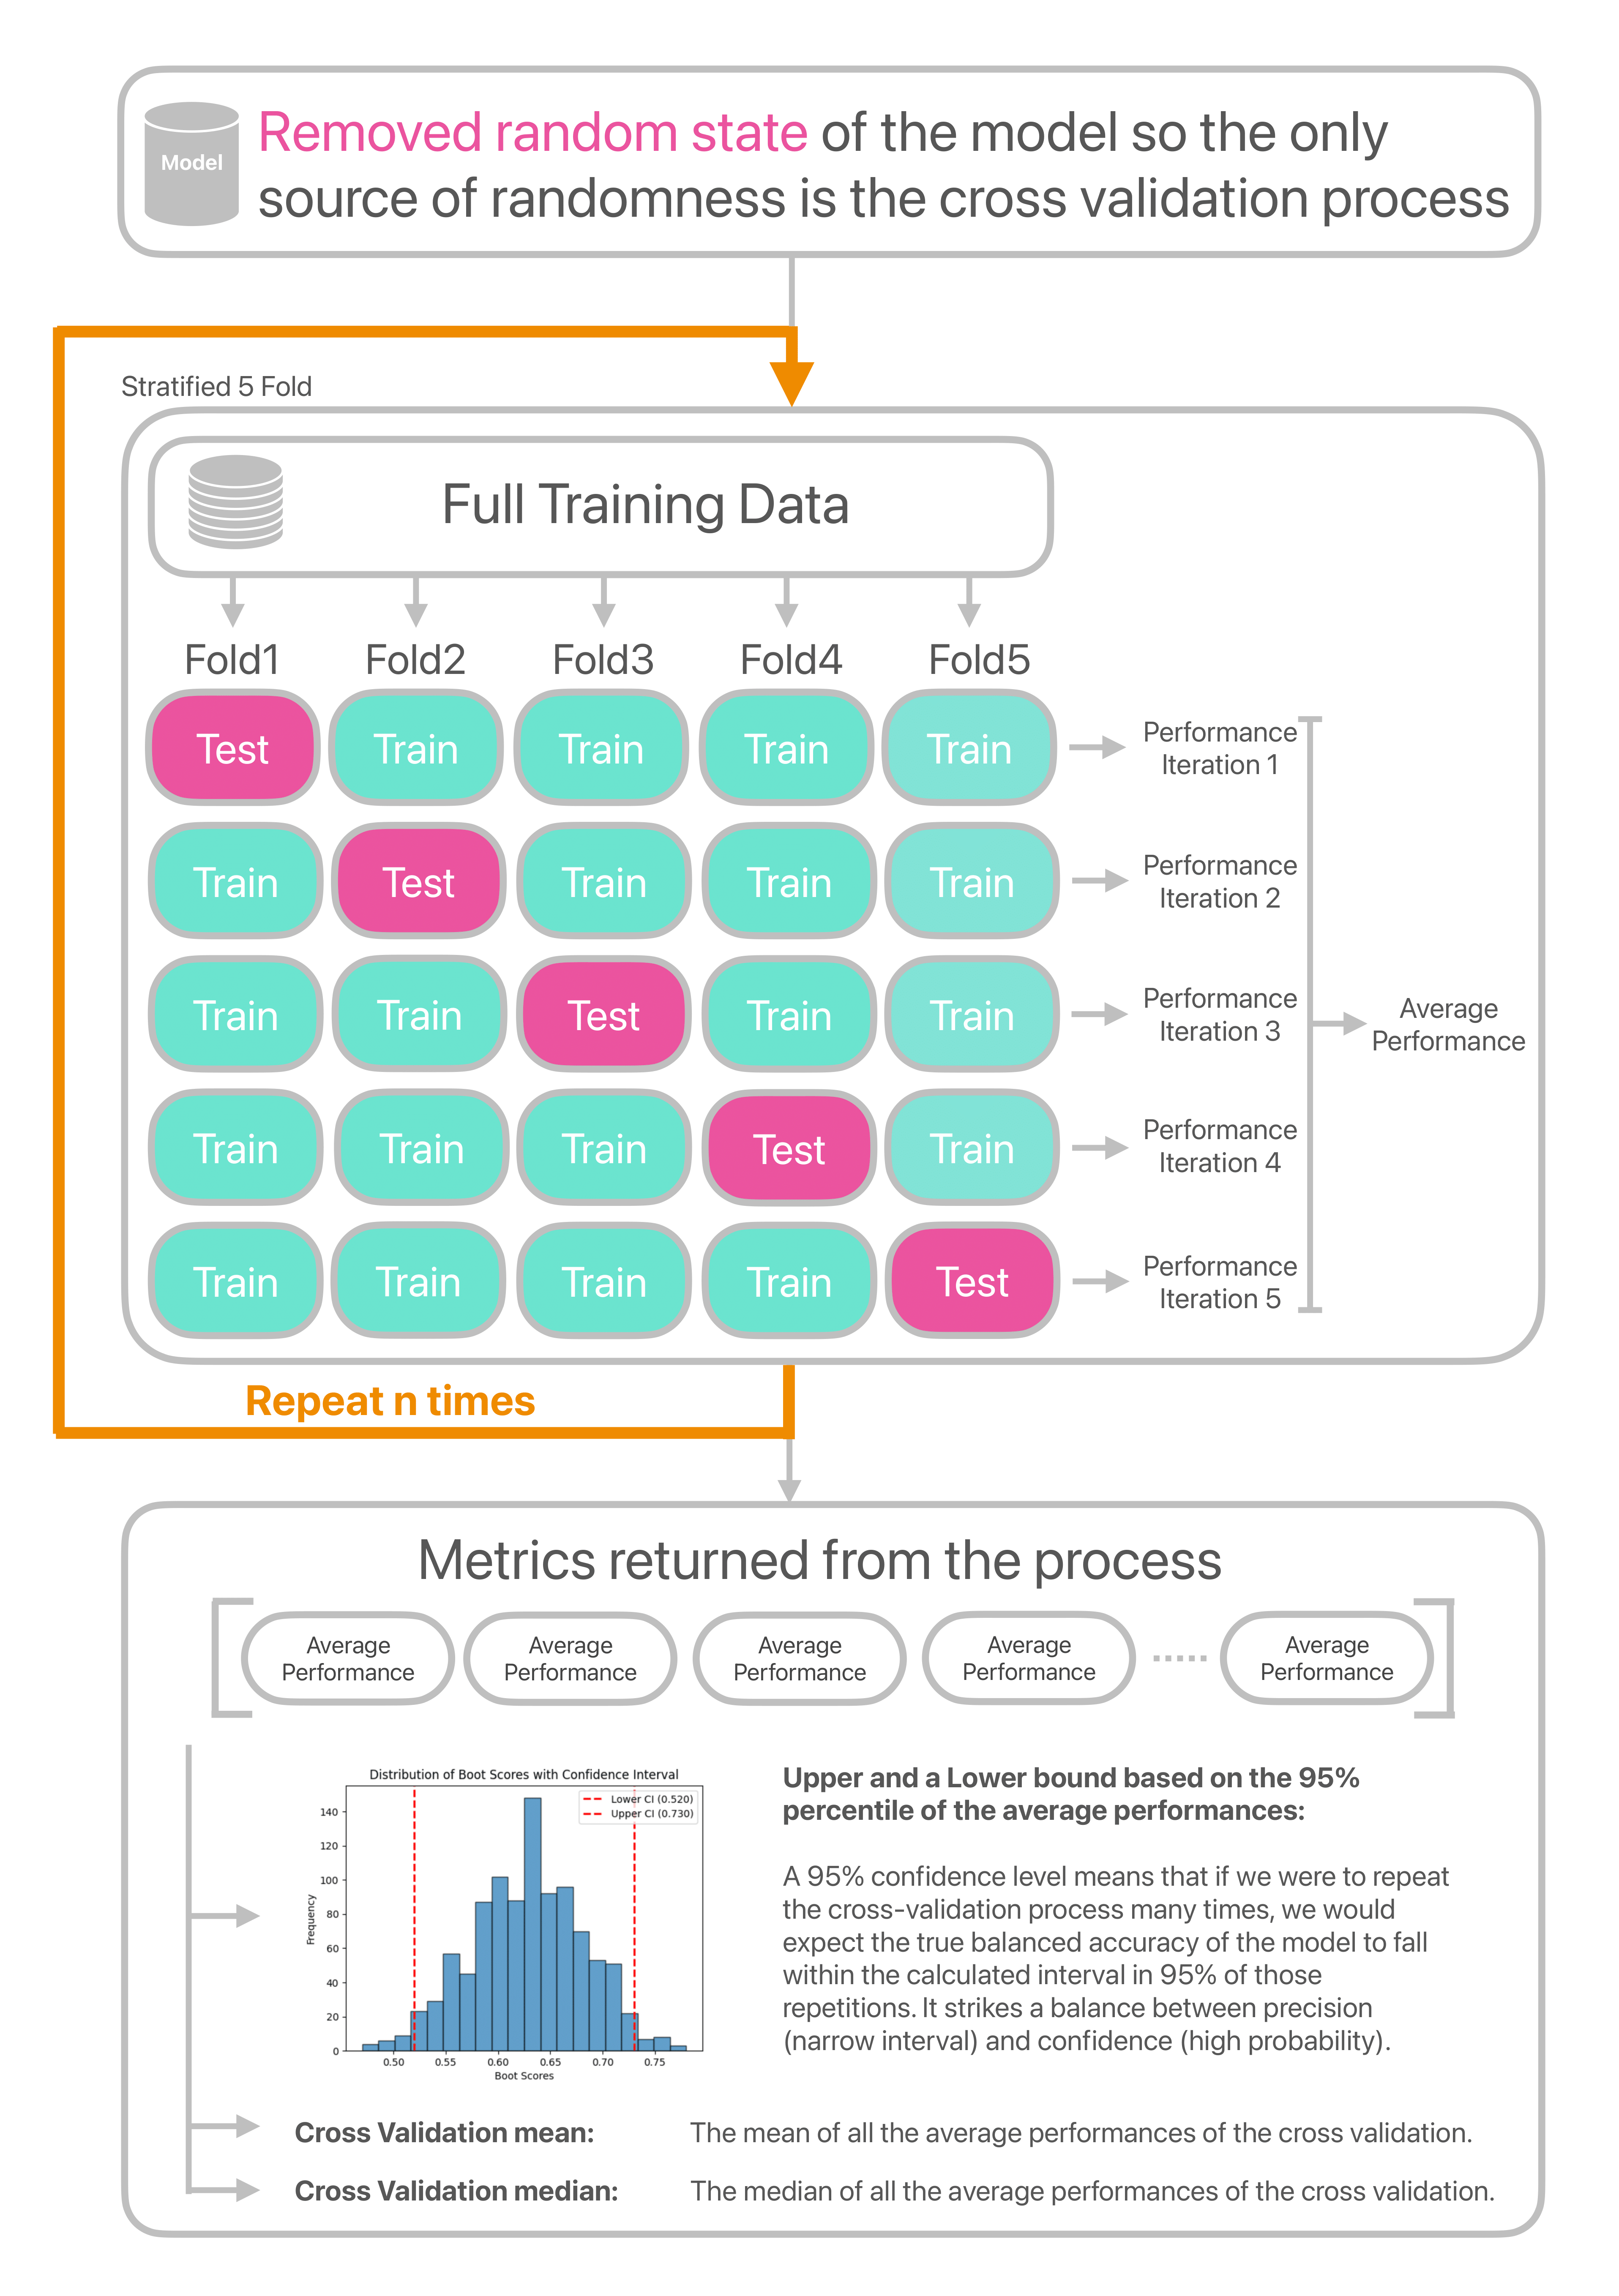
\includegraphics[width=0.9\textwidth]{images/Bootstrapping-1.png}
  \caption[Confidence interval estimation diagram using repeated stratified 5-fold cross-validation]{This diagram illustrates the process of estimating the confidence interval of a model's performance using repeated stratified k-fold cross-validation. Initially, the model's random state is removed to ensure the cross-validation process is the sole source of randomness. Stratified k-fold cross-validation (k=5) is used to evaluate model performance, with the average score across folds representing a single iteration's result. This entire cross-validation procedure is repeated 'n' times (e.g., 1000) to simulate the variability in performance across different random splits. The resulting 'n' average performance scores are then used to calculate the confidence interval. These bounds indicate the range within which we expect the model's true performance to lie with a high degree of confidence, providing a robust measure of the model's reliability.}
  \label{fig:Bootstrapping-1}
\end{figure}

\begin{figure}[H]
  \centering
  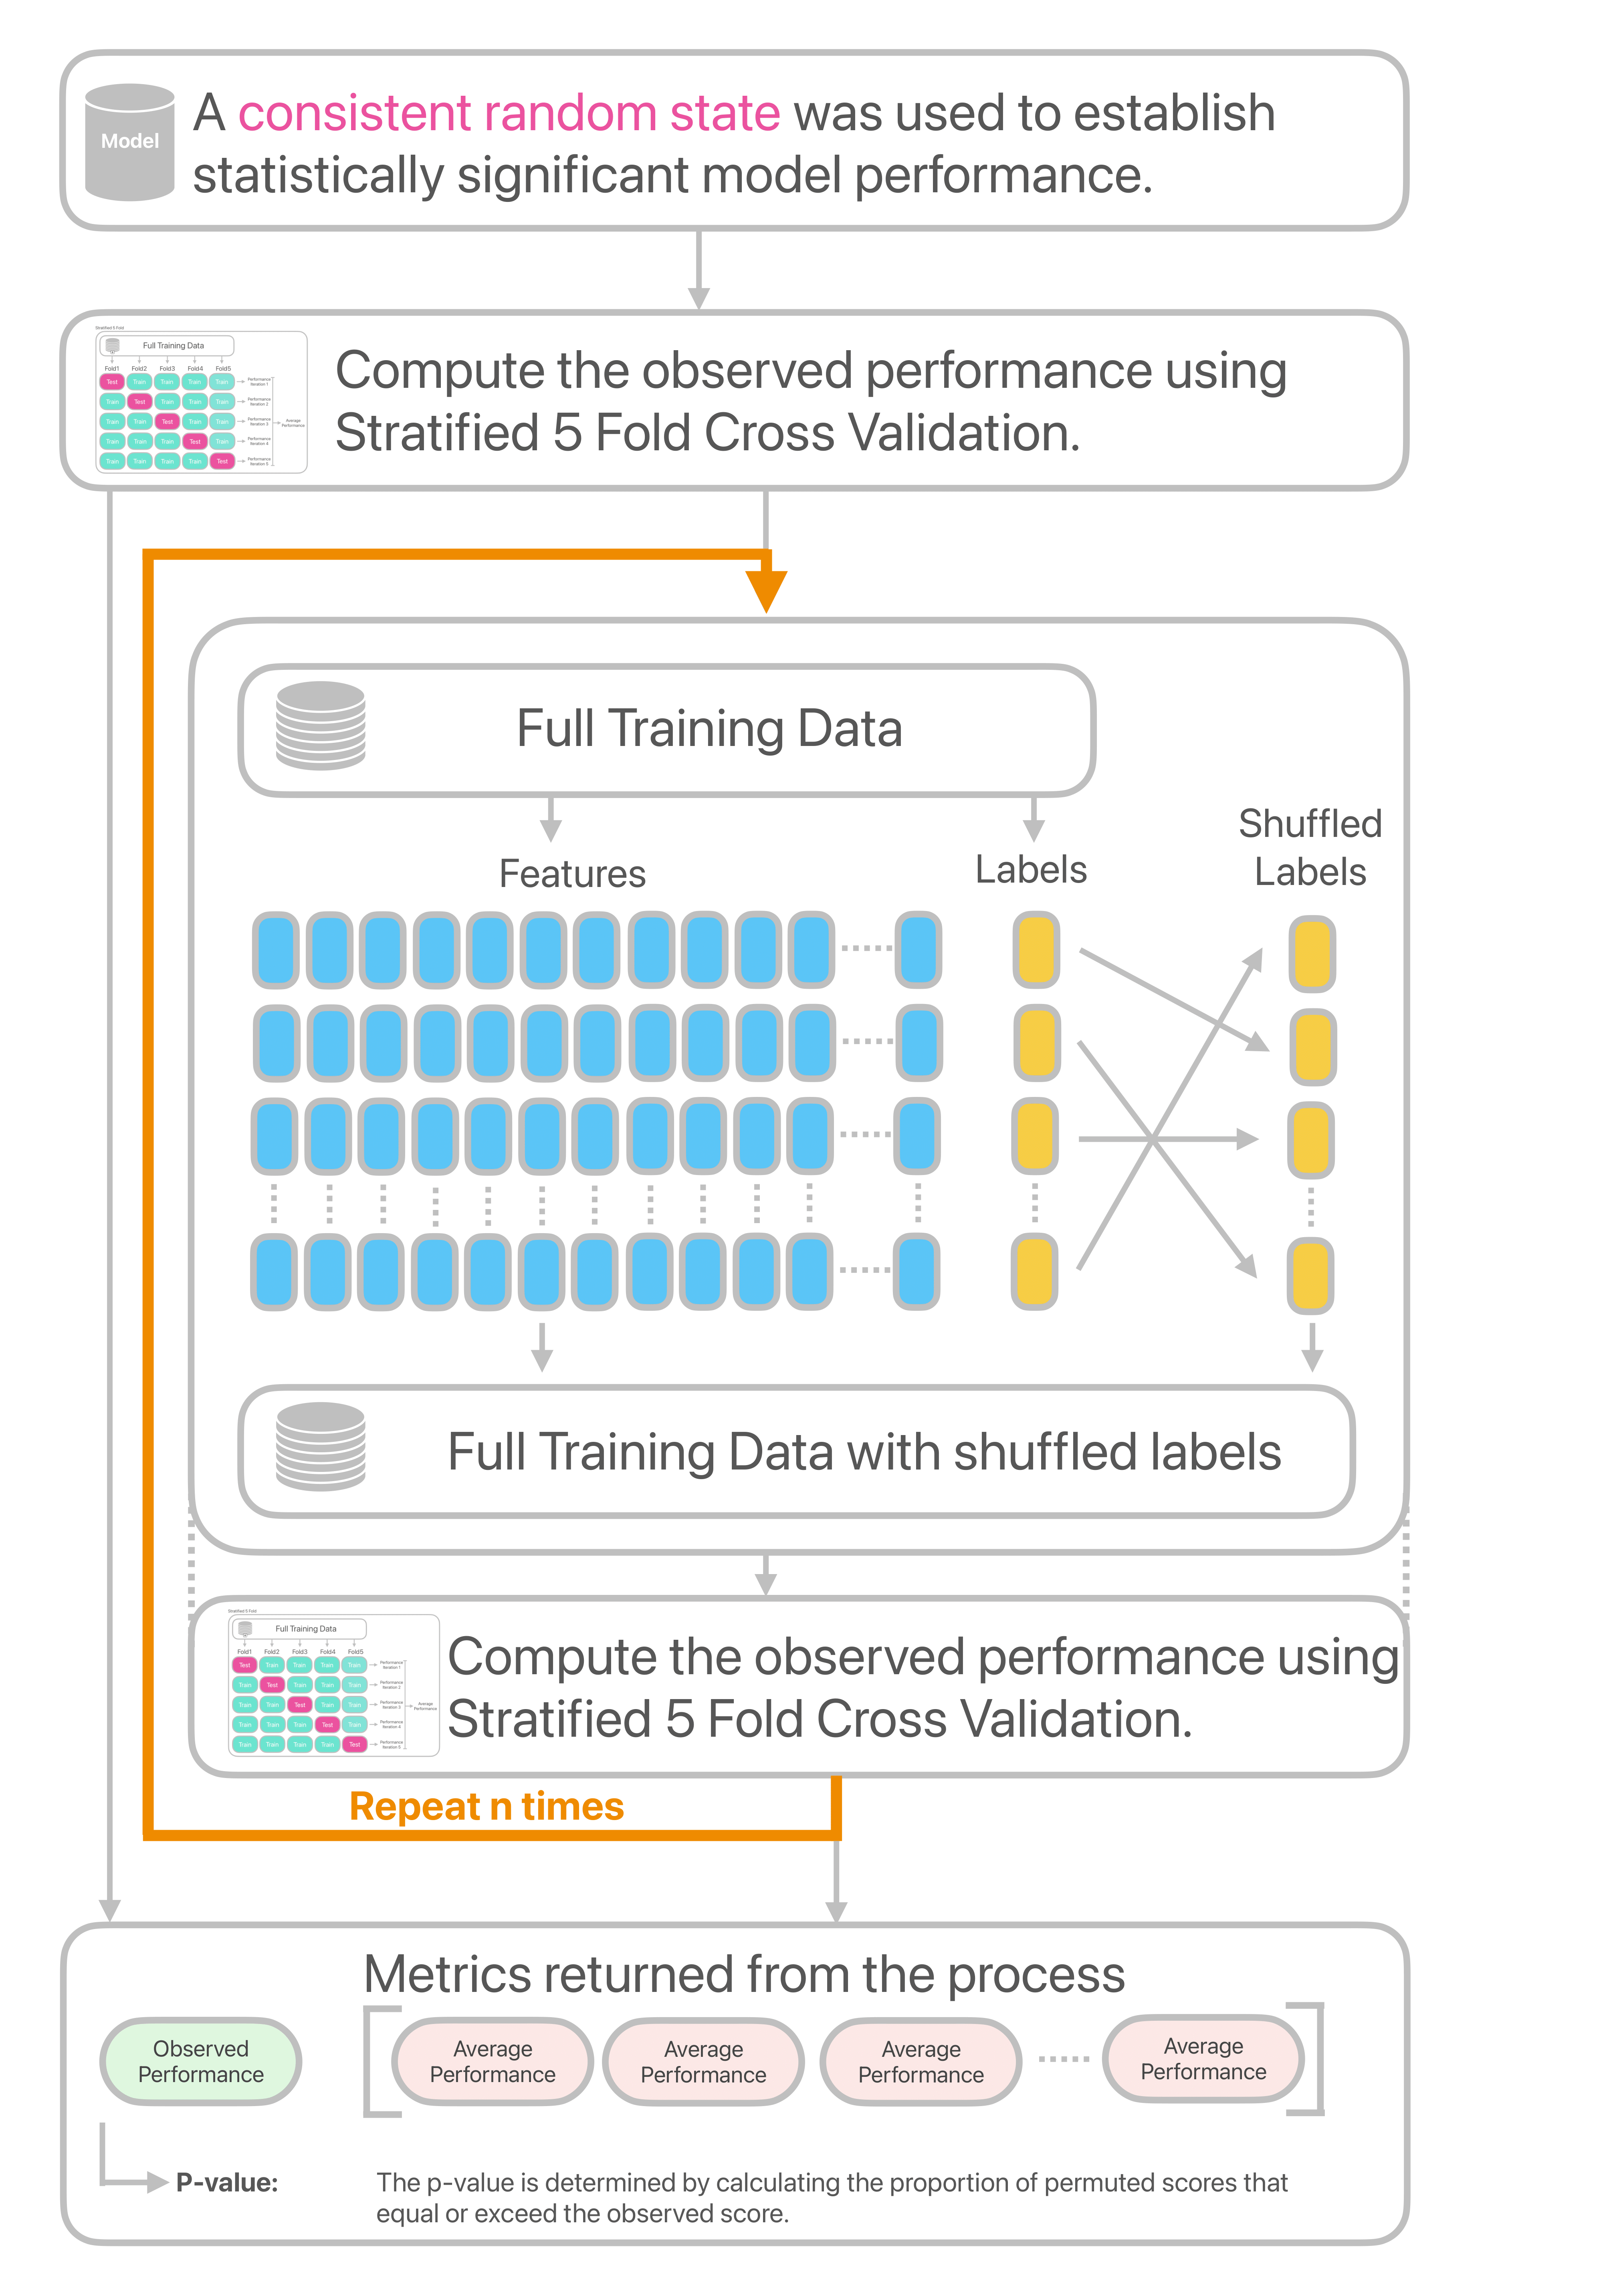
\includegraphics[width=0.9\textwidth]{images/P-value_test-1.png}
  \caption[Evaluating model significance via permutation testing and p-value calculation diagram]{This diagram illustrates a permutation test designed to evaluate the statistical significance of a model's performance. Initially, a consistent random state is set to ensure reproducible results. The model's performance is first assessed on the original data using stratified 5-fold cross-validation, yielding the 'observed performance.' Subsequently, to determine if this performance is merely due to chance, the labels are repeatedly shuffled. For each shuffled dataset, the model's performance is re-evaluated using the same stratified 5-fold cross-validation. This process is repeated 'n' times, resulting in a distribution of 'permuted performances.' Finally, the p-value is calculated as the proportion of permuted performances that equal or exceed the observed performance, indicating the likelihood of obtaining such performance by chance alone.}
  \label{fig:P-value_test-1}
\end{figure}


\subsection{Findings for Consensus model}
\label{sec:findings_for_consensus_model}
\noindent
A primary observation was the marked heterogeneity in the optimal modeling strategies across the different data types, supporting the core premise of the multi-pipeline approach. When utilizing the original, uncompressed features, the best-performing configurations (selected based on validation set performance, with CV MEAN and p-value as tie breakers), are summarized below:
\begin{table}[H]
    \centering
    \hspace*{-1cm}
    \scalebox{0.8}{%
    \begin{tabular}{l l l l l l l}
        \toprule
        Data Type & Oversampling & Best Model & Train Balanced Acc. & Train $p$-value & Val. F1 & Val. Balanced Acc. \\
        \midrule
        cytokines & smote & Logistic Regression & 0.712 & 0.010 & 0.815 & 0.750 \\
        cytometry & smote & Logistic Regression & 0.724 & 0.045 & 0.815 & 0.750 \\
        clonal breadth & random & Naive Bayes & 0.655 & 0.099 & 0.500 & 0.667 \\
        clonal depth & smote & Decision Tree & 0.559 & 0.154 & 0.767 & 0.833 \\
        \acrshort{rna} & smote & Random Forest & 0.810 & 0.000 & 0.514 & 0.500 \\
        \bottomrule
    \end{tabular}}
    \caption[Optimal Modeling Configurations Uncompressed Features]{Optimal Modeling Configurations for Uncompressed Features}
    \label{tab:optimal_configs_uncompressed}
\end{table}

\noindent
The best-performing model for each data type generated the following predictions on their respective test sets: for cytokines, the prediction was $[1\ 1\ 1\ 0\ 0\ 0]$ with a test accuracy of 0.333; for cytometry, the prediction was $[1\ 0\ 0\ 0\ 0\ 0]$ with a test accuracy of 0.667; for clonal breadth, the prediction was $[1\ 0\ 0\ 1\ 0\ 0]$ with a test accuracy of 0.500; for clonal depth, the prediction was $[0\ 0\ 0\ 0\ 1\ 0]$ with a test accuracy of 1.0; and for \acrshort{rna}, the prediction was $[0\ 1\ 0\ 0\ 1\ 0]$ with a test accuracy of 0.833.\\
\\
A consensus prediction was derived by applying majority voting across these individual model outputs, resulting in a final prediction of $[1\ 0\ 0\ 0\ 0\ 0]$. This consensus prediction was then evaluated against the true labels which were $[0\ 0\ 0\ 0\ 1\ 0]$.\\
\\
The overall performance of the consensus prediction on the test set yielded an accuracy of 0.667 and a balanced accuracy of 0.400. A more detailed breakdown of the consensus performance is provided by the classification report:
\begin{table}[h!]
    \centering
    \scalebox{0.8}{%
    \begin{tabular}{l c c c c}
        \toprule
        Class & Precision & Recall & F1-Score & Support \\
        \midrule
        0 & 0.80 & 0.80 & 0.80 & 5 \\
        1 & 0.00 & 0.00 & 0.00 & 1 \\
        \midrule
        Accuracy &       &      & 0.67 & 6 \\
        Macro Avg & 0.40 & 0.40 & 0.40 & 6 \\
        Weighted Avg & 0.67 & 0.67 & 0.67 & 6 \\
        \bottomrule
    \end{tabular}}
    \caption[Consensus Classification Report Uncompressed Features]{Consensus Classification Report for Uncompressed Features}
    \label{tab:consensus_report_uncompressed}
\end{table}

\noindent
Further investigation involved applying \gls{pca}-based feature compression within each pipeline. This led to a different set of optimal configurations:
\begin{table}[H]
    \centering
    \hspace*{-1cm}
    \scalebox{0.8}{%
    \begin{tabular}{l l l l l l l}
        \toprule
        Data Type & Oversampling & Best Model & Train Balanced Acc. & Train $p$-value & Val. F1 & Val. Balanced Acc. \\
        \midrule
        cytokines & random & Naive Bayes & 0.630 & 0.076 & 0.815 & 0.750 \\
        cytometry & smote & Decision Tree & 0.725 & 0.009 & 0.815 & 0.750 \\
        clonal breadth & random & Naive Bayes & 0.655 & 0.099 & 0.500 & 0.667 \\
        clonal depth & smote & Decision Tree & 0.559 & 0.154 & 0.767 & 0.833 \\
        \acrshort{rna} & smote & Logistic Regression & 0.789 & 0.011 & 0.667 & 0.625 \\
        \bottomrule
    \end{tabular}}
    \caption[Optimal Modeling Configurations Compressed Features]{Optimal Modeling Configurations for Compressed Features}
    \label{tab:optimal_configs_compressed}
\end{table}
\noindent
The best-performing model for each data type generated the following predictions on their respective test sets: for cytokines, the prediction was $[0\ 0\ 0\ 0\ 0\ 0]$ with a test accuracy of 0.833; for cytometry, the prediction was $[1\ 0\ 0\ 0\ 0\ 0]$ with a test accuracy of 0.667; for clonal breadth, the prediction was $[1\ 0\ 0\ 1\ 0\ 0]$ with a test accuracy of 0.500; for clonal depth, the prediction was $[0\ 0\ 0\ 0\ 1\ 0]$ with a test accuracy of 1.0; and for \acrshort{rna}, the prediction was $[0\ 1\ 0\ 0\ 0\ 0]$ with a test accuracy of 0.667.\\
\\
A consensus prediction was derived by applying majority voting across these individual model outputs, resulting in a final prediction of $[0\ 0\ 0\ 0\ 0\ 0]$. This consensus prediction was then evaluated against the true labels which were $[0\ 0\ 0\ 0\ 1\ 0]$.\\
\\
The overall performance of the consensus prediction on the test set yielded an accuracy of 0.833 and a balanced accuracy of 0.500. A more detailed breakdown of the consensus performance is provided by the classification report:
\begin{table}[h!]
    \centering
    \scalebox{0.8}{%
    \begin{tabular}{l c c c c}
        \toprule
        Class & Precision & Recall & F1-Score & Support \\
        \midrule
        0 & 0.83 & 1.00 & 0.91 & 5 \\
        1 & 0.00 & 0.00 & 0.00 & 1 \\
        \midrule
        Accuracy &       &      & 0.83 & 6 \\
        Macro Avg & 0.42 & 0.50 & 0.45 & 6 \\
        Weighted Avg & 0.69 & 0.83 & 0.76 & 6 \\
        \bottomrule
    \end{tabular}}
    \caption[Consensus Classification Report Compressed Features]{Consensus Classification Report for Compressed Features}
    \label{tab:consensus_report_compressed}
\end{table}

\noindent
The consensus prediction based on majority voting of individual data-type specific models trained on the original, uncompressed features achieved an accuracy of 0.667 and a balanced accuracy of 0.400 on the test set.\\
\\
Applying \gls{pca}-based feature compression within each pipeline resulted in a different set of optimal configurations for some data types. The consensus prediction from these models, evaluated on the test set, showed an accuracy of 0.833 and a balanced accuracy of 0.500. These results indicate that for this dataset, the use of compressed features yielded better overall and balanced accuracy in the consensus prediction compared to the uncompressed feature approach.\\
\\
The optimal configurations identified across most data types consistently utilized either \gls{smote} or random oversampling techniques. This highlights the importance of addressing class imbalance to optimize the performance of the individual models. Oversampling likely helped the models to better capture the characteristics of the minority class, mitigating the tendency to predominantly predict the majority class.\\
\\
Several limitations should be acknowledged when interpreting The findings presented so far. The most significant constraint is the very small size of the test set ($n=6$), which severely limits the statistical power of the performance metrics and the generalizability of the results. The precision of an estimate of the performance outside the sample is heavily dependent on the absolute size of the validation or test set ($n$). This relationship is quantitatively expressed by the formula for the standard error of the measured accuracy: $\sqrt{p(1-p)/n}$, where $p$ is the true accuracy. A smaller standard error indicates that the measured accuracy is likely closer to the true accuracy.\\
\\
For a test set size of $n=6$, the uncertainty is substantial. Using the formula, the standard error is largest when $p=0.5$, resulting in a standard error of $\sqrt{0.5 \times 0.5 / 6} = \sqrt{0.25 / 6} \approx \sqrt{0.0417} \approx 0.204$. This translates to a standard error of roughly 20.4\%. Even at higher accuracies, such as $p=0.8$, the standard error remains considerably large: $\sqrt{0.8 \times 0.2 / 6} = \sqrt{0.16 / 6} \approx \sqrt{0.0267} \approx 0.163$, or about 16.3\%.\\
\\
This magnitude of standard error implies that any accuracy value calculated on this 6-sample test set is a very imprecise estimate of the model's true performance. If, for instance, the model achieved an accuracy of 0.667 (4 out of 6 correct), the true accuracy could plausibly be significantly higher or lower purely due to random chance in the selection of these 6 samples. Similarly, an accuracy of 0.833 (5 out of 6 correct) also carries a large margin of error. This contrasts sharply with scenarios requiring validation sets in the hundreds of thousands to achieve very small standard errors (e.g., 0.1\% or 1\%).\\
\\
Looking at this from another perspective, the small sample size directly impacts the width of confidence intervals, such as the Clopper-Pearson interval, which is often used for proportions based on small sample sizes. The Clopper-Pearson interval provides an exact confidence interval for binomial proportions, especially appropriate for small samples or cases when the normal approximation might fail. It gives us a range within which we are confident that the "true accuracy" or "true proportion" actually lies, based on our observed data. This method calculates the confidence interval by identifying all values of the true proportion $p$ for which the observed data would be reasonably likely, given the chosen confidence level.\\
\\
The interval is computed based on the cumulative probabilities of the binomial distribution. Mathematically, for an observed proportion $\hat{p} = x/n$ (where $x$ is the number of successes in
$n$ trials), the Clopper-Pearson interval at a confidence level $1-\alpha$ is given by the bounds:
\[
\text{Lower bound} = \text{BetaInv}\left(\frac{\alpha}{2};\, x,\, n - x + 1\right)
\]

\[
\text{Upper bound} = \text{BetaInv}\left(1 - \frac{\alpha}{2};\, x + 1,\, n - x\right)
\]
where BetaInv denotes the inverse of the cumulative Beta distribution function. While the Clopper-Pearson method is based on binomial probabilities rather than a simple formula involving standard error, it is fundamentally driven by the same underlying sampling variability. Increasing the sample size ($n$) reduces this variability, leading to a smaller standard error and, consequently, a narrower Clopper-Pearson confidence interval. For our test set of $n=6$, the resulting confidence intervals for the observed accuracies are very wide. For an observed accuracy of 0.667 (4/6), the 95\% Clopper-Pearson confidence interval is approximately $[0.299, 0.925]$, a width of about 0.626. For an observed accuracy of 0.833 (5/6), the 95\% confidence interval is approximately $[0.359, 0.996]$, a width of about 0.637. This shows that even with a measured accuracy of 0.833, the true accuracy could plausibly be as low as around 36\% due to the limited sample size.\\
\\
Given that simple majority voting did not produce exceptional consensus results, further exploration of more sophisticated ensemble aggregation methods was not pursued in this study. Future work could investigate techniques such as weighted voting (where individual model contributions are weighted based on factors like validation performance or modality relevance), stacking (employing a meta-learner to combine predictions), or rank aggregation, which may potentially lead to more robust and balanced consensus predictions.




%\section{SMOTE-Driven Oversampling and SHAP-Based Feature Interpretation Approach}

\section{Feature Identification Methodology}
\noindent
Given the constraints imposed by the limited dataset ($N=40$), particularly the small number of samples available for independent testing, a primary objective of this study was to explore and identify potentially important features associated with the vaccine response. Standard approaches for model selection and rigorous performance evaluation typically rely on larger validation or test sets to provide reliable estimates of out-of-sample performance and prevent overfitting during the selection process. However, as discussed in the previous section, the extremely small size of our test set ($n=6$) introduces substantial uncertainty into any performance metric, as demonstrated by the large standard errors and wide Clopper-Pearson confidence intervals. While a test set size of $n=8$ offers a marginal improvement in reducing the width of the confidence interval compared to an even smaller sample like $n=6$, it still leaves a significant degree of uncertainty, rendering traditional rigorous model selection based on distinct validation/test splits highly problematic and potentially less informative than desired.\\
\\
Recognizing these severe data limitations, the approach to feature identification prioritizes exploration and hypothesis generation. A variety of models were trained (see Table~\ref{tab:ml_models}) across different data types, incorporating various \gls{smote} oversampling variations to address the inherent class imbalance in the dataset. To understand the contribution of individual features within these models, I utilized \acrfull{shap} \cite{ApprouchForModelPredictions} values. It is a technique that explains the output of machine learning models by assigning each feature an importance value based on its contribution to the model’s predictions using game theory.

\subsection{Pipeline Structure for Heterogeneous Datasets}
\label{subsec:pipeline_structure_for_Heterogeneous_datasets}
To systematically implement the exploratory strategy outlined above, a standardized computational pipeline was employed (very similar to the pipeline in Section~\ref{sec:consensus_model_approach}). This pipeline, visually detailed in Figure~\ref{fig:pipeline-2}, ensures consistency in data handling, model training, and the generation of performance metrics across all experimental conditions. It encompasses crucial steps from initial data preprocessing and targeted oversampling of the training data to model fitting and the assessment of performance on the hold-out test set. The models generated and evaluated through this workflow form the basis for the subsequent performance filtering and aggregation of \gls{shap} values aimed at identifying potentially important features. The following sections describe each stage of this pipeline.

\begin{figure}[H]
  \centering
  \hspace*{-0.9cm} % Adjust spacing as needed
  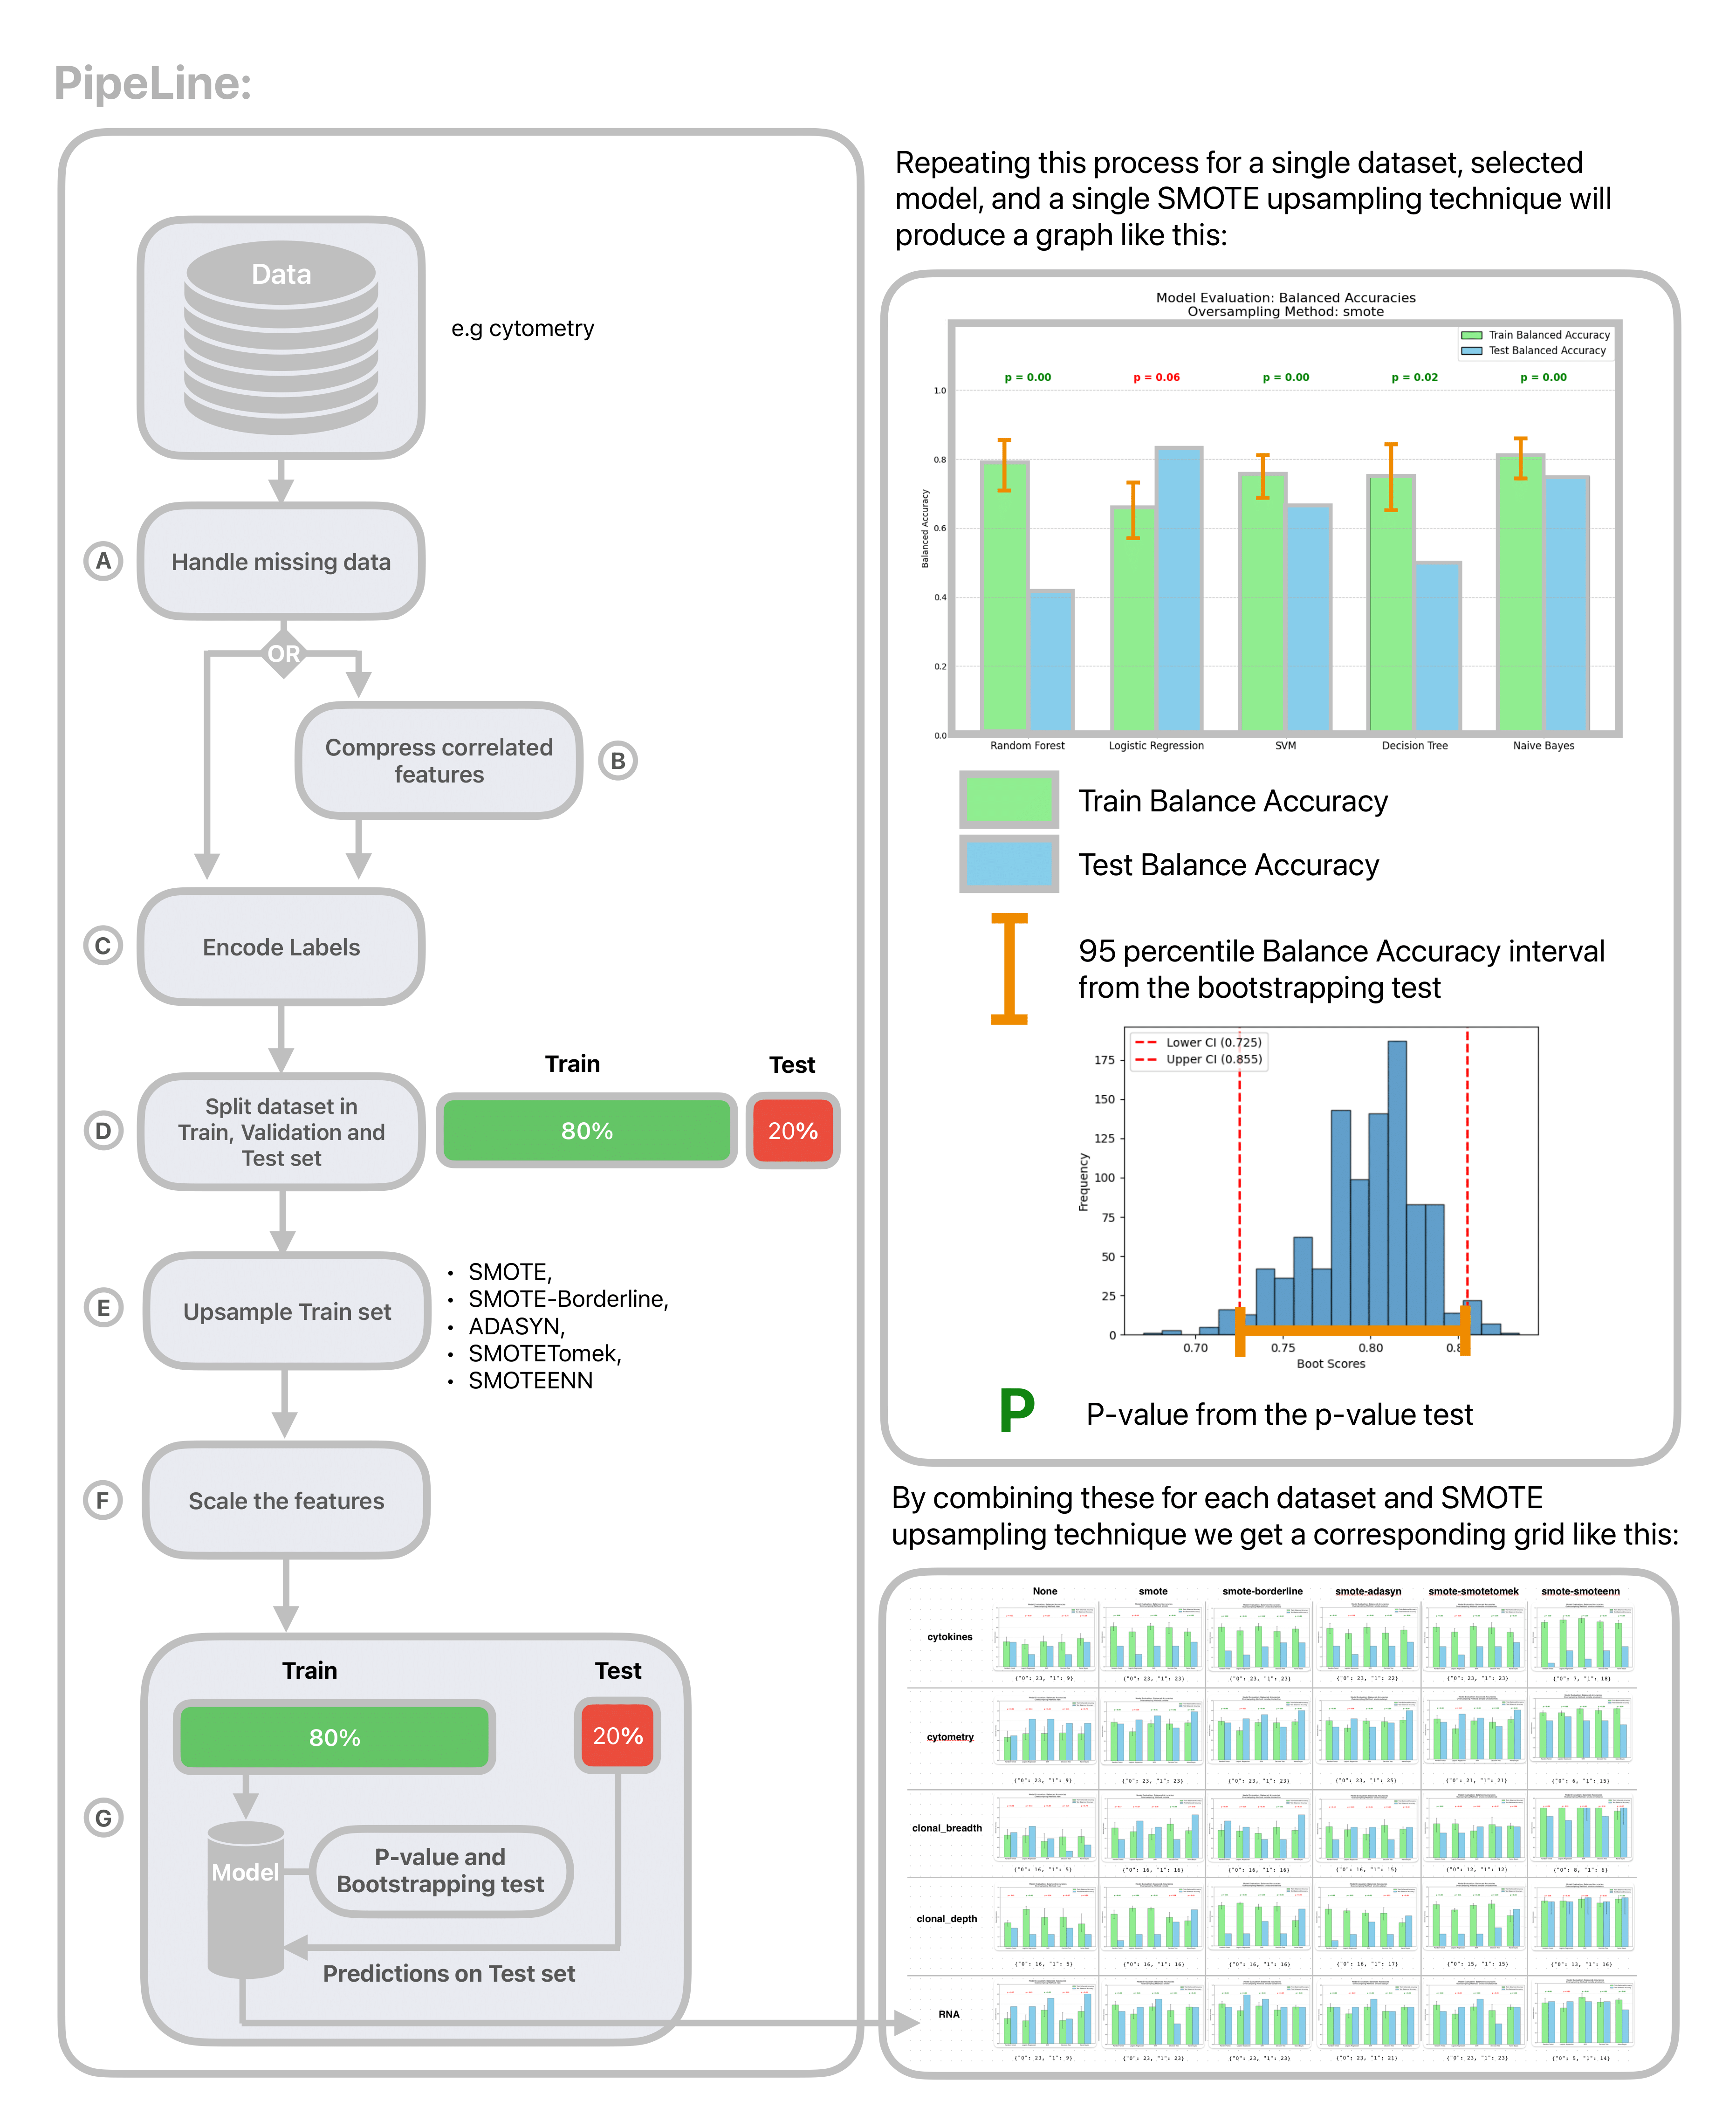
\includegraphics[width=1.1\textwidth]{images/Pipeline-2.png} % Ensure path is correct
  \caption[Feature Identification models pipeline diagram]{ The diagram illustrates the multi-model pipeline used for constructing the models.  Each individual model follows a standardized preprocessing workflow: data loading, preprocessing (A: Missing data handling, B: Feature compression, C: Label encoding, F: Feature scaling), data splitting (D), training set oversampling using various \gls{smote} techniques (E), model training, and evaluation (G). Performance on train and test sets is measured by Balanced Accuracy, with 95\% bootstrap confidence intervals and p-value testing, repeated across datasets and \gls{smote} methods as illustrated.}
  \label{fig:pipeline-2}
\end{figure}

\subsubsection{Preprocessing \hyperref[fig:pipeline-2]{(A, B, C, F)}}
\noindent The initial data preparation steps, specifically handling missing data \hyperref[fig:pipeline-2]{(A)}, compressing correlated features \hyperref[fig:pipeline-2]{(B)}, and encoding class labels \hyperref[fig:pipeline-2]{(C)}, and later scaling the features \hyperref[fig:pipeline-2]{(F)}, were performed using the identical procedures as detailed in Section~\ref{sec:consensus_model_approach}.

\subsubsection*{Split dataset \hyperref[fig:pipeline-2]{(D)}}
As mentioned earlier, due to the extreme data scarcity ($N=40$), the decision was made to partition the data into a training set comprising of 80\% of the samples ($n=32$) and a hold-out test set containing the remaining 20\% ($n=8$). Further splitting the training data to create a separate validation set would drastically reduce the number of samples available for model training, likely impairing the models' ability to learn meaningful patterns from the data. Furthermore, dividing the test set further would make the individual subsets too small to yield any statistically stable or meaningful performance estimates as discussed in the previous Section~\ref{sec:findings_for_consensus_model}. Therefore, I made the pragmatic decision to use the performance observed \textit{only} on the hold-out test set ($n=8$) as a preliminary criterion for filtering models whose \gls{shap} explanations would be further analyzed and aggregated.\\
\\
While conventionally using the test set for model selection is strongly discouraged due to the risk of test set overfitting and obtaining overly optimistic performance estimates, the extreme data scarcity in this study necessitates this deviation from standard practice. I utilized the performance on the $n=8$ test set, which was explicitly constructed with 4 positive (responder) and 4 negative (non-responder) samples. This specific balanced split, rather than a purely stratified one, was chosen to ensure adequate representation of both minority and majority classes within the extremely limited test cohort, thereby allowing for a more meaningful assessment of the model's ability to distinguish between responders and non-responders even with very few samples.\\
\\
The performance on this n=8 test set is used not for precise model ranking or performance reporting, but primarily as a coarse filter. Models that perform poorly even on this small test set are excluded, as their low scores, despite the uncertainty, suggest they are unlikely to generalize well. Conversely, models that achieve higher scores on this $n=8$ test set are retained. While the uncertainty on an $n=8$ sample means that a high score does not guarantee good true performance, these models still possess the potential to be good performers. Excluding them based on the high variance associated with the $n=8$ estimate would be overly conservative and might discard promising candidates for feature analysis. This approach is used with the explicit understanding that it is a pragmatic compromise driven by data constraints. The subsequent findings regarding feature importance derived from aggregating \gls{shap} values of these filtered models are to be interpreted strictly as exploratory hypotheses rather than definitive conclusions. The goal is to identify features that appear consistently important across models that show some minimal indication of potential relevance on the limited unseen data, providing potential candidates for validation in future studies with larger datasets.

\subsubsection*{Up-sample Train set \hyperref[fig:pipeline-2]{(E)}}
It became evident that strategies involving data upsampling, such as random oversampling and particularly \gls{smote}, played a crucial role in improving model performance when dealing with small, imbalanced datasets. Motivated by these findings, I extended the analysis to investigate several variations of \gls{smote}. These methods aim to address class imbalance more effectively than standard \gls{smote} by refining the process of generating synthetic samples or combining it with data cleaning techniques, thereby allowing models to extract more useful patterns and generalize better from sparse data.\\
\\
The first method used was standard \gls{smote} \cite{Chawla2002SMOTE}, which, as previously detailed in Subsection~\ref{subsec:pipeline_structure_for_heterogeneous_datasets} (Up-sample Train set), synthesizes new minority instances by generating samples along the lines connecting existing minority samples and their selected k-nearest minority neighbors (illustrated conceptually in Figure~\ref{fig:SMOTE_explained}). Standard \gls{smote}, while a foundational technique, has known weaknesses, as detailed in Subsection~\ref{subsec:pipeline_structure_for_heterogeneous_datasets} and conceptually illustrated in Figure~\ref{fig:SMOTE_weaknesses}. The variations of \gls{smote} included in this study were developed to mitigate these issues, either by focusing synthetic sample generation on more informative areas or by combining oversampling with data cleaning steps.\\
\begin{figure}[h!]
  \centering
  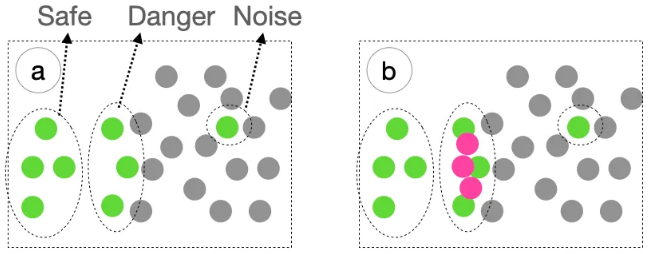
\includegraphics[width=0.9\textwidth]{images/SMOTE-Borderline.png}
  \caption[Illustration of Borderline-\gls{smote} Sample Generation]{Illustration of the Borderline-\gls{smote} synthetic sample generation process. Panel (a) shows minority class samples (green) categorized into 'Safe', 'Danger' (borderline), and 'Noise' zones based on the ratio of majority class neighbors (grey) among their k-nearest neighbors. Panel (b) demonstrates how synthetic minority samples (pink) are generated specifically in the 'Danger' zone. Figure adapted from figure 9 presented in \cite{Truong2022SMOTEVariants}.}
  \label{fig:SMOTE-Borderline}
\end{figure}
\\
\noindent
As a prime example of a variation focusing on challenging areas, Borderline-\gls{smote} \cite{Han2005Borderline} was applied. Proposed by Han et al. in 2005, this variant is based on the reasoning that minority samples located in the borderline regions near the decision boundary are particularly difficult for classifiers to learn. By specifically adding more synthetic samples in these ambiguous regions, the method aims to help the classifier distinguish between classes better. The core idea of Borderline-\gls{smote} is to first identify minority samples that are in 'danger' of being misclassified. Using k-nearest neighbors (\acrshort{kknn}), each minority sample is classified into a 'noise', 'safe' or 'danger' zone based on the ratio ($r$) of majority instances among its neighbors. A sample is considered 'noise' if all its neighbors are majority class ($r=1$), in a 'safe' zone if most neighbors are minority class ($r < 0.5$), and in the 'danger' (or 'borderline') zone if the mix is significant ($0.5 \leq r < 1$). Unlike standard \gls{smote} which oversamples all minority samples, Borderline-\gls{smote} focuses its synthetic sample generation only on those minority samples identified as being in the 'danger' zone, synthesizing new instances by interpolating between a danger-zone sample and its minority neighbors. This targeted approach aims to reinforce the decision boundary in regions considered critical for classification, as illustrated in Figure~\ref{fig:SMOTE-Borderline}.\\
\begin{figure}[h!]
  \centering
  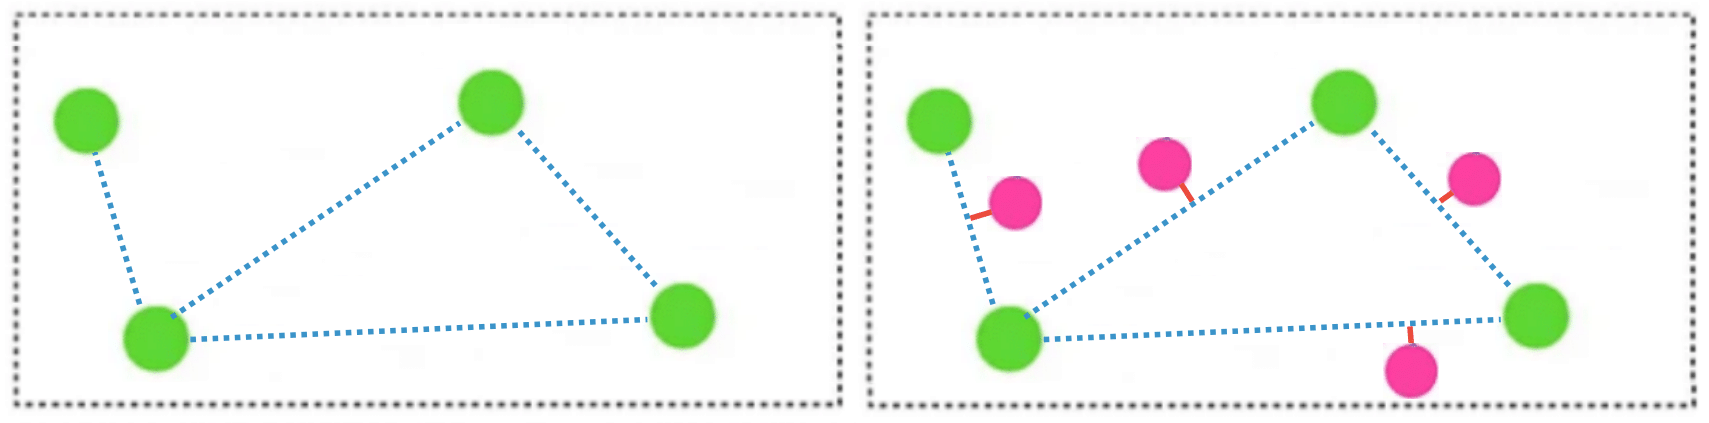
\includegraphics[width=0.9\textwidth]{images/SMOTE-ADASYN.png}
  \caption[Illustration of \acrshort{adasyn} Sample Generation]{Illustration of the \acrshort{adasyn} synthetic sample generation process. The left panel shows original minority samples. The right panel shows synthetic minority samples (pink) generated by \acrshort{adasyn}, demonstrating the addition of small random variations that cause the synthetic points to be slightly scattered around the interpolation lines between neighbors. Figure made in same style as images presented in \cite{Truong2022SMOTEVariants}.}
  \label{fig:SMOTE-ADASYN}
\end{figure}
\\
\noindent
Another approach included was \gls{adasyn} \cite{He2008ADASYN}. Presented as an improved version of standard \gls{smote}, \gls{adasyn} incorporates a modification to the synthetic sample generation process. After creating synthetic points via interpolation similar to \gls{smote}, \gls{adasyn} adds small random values $\lambda \in [0, 1]$ to these generated points. This addition introduces a degree of variance, resulting in synthetic samples that are slightly scattered around the interpolating line rather than being strictly linearly correlated with the original samples, as illustrated in Figure~\ref{fig:SMOTE-ADASYN}. This aims to make the generated data distribution more realistic and potentially help models generalize better.\\
\begin{figure}[h!]
  \centering
  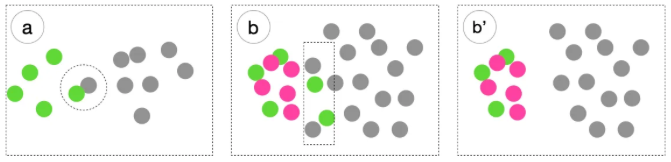
\includegraphics[width=0.9\textwidth]{images/SMOTE-Tomek.png}
  \caption[Illustration of \gls{smote}-Tomek Process]{Illustration of the \gls{smote}-Tomek process. Panel (a) conceptually shows a Tomek link, defined as a pair of instances from different classes that are mutual nearest neighbors. Panel (b) depicts a dataset after standard \gls{smote} oversampling, including original (green and grey) and synthetic (pink) samples. Panel (b') shows the result after the removal of Tomek links, which helps to clean the decision boundary by eliminating ambiguous points near the interface between classes. Figure adapted from figure 5 presented in \cite{Truong2022SMOTEVariants}.}
  \label{fig:SMOTE-Tomek} % Corrected label spelling
\end{figure}
\\
\noindent
Furthermore, hybrid techniques combining \gls{smote} oversampling with data cleaning were also included in the analysis pipeline. \gls{smote}-Tomek \cite{Batista2004Study} implements a two-stage process. It first applies standard \gls{smote} to oversample the minority class, and then utilizes the concept of Tomek links to perform a cleaning step. A Tomek link is defined as a pair of instances $(x_i, x_j)$ from different classes that are mutual closest neighbors, meaning $x_i$ is the nearest neighbor of $x_j$, and $x_j$ is the nearest neighbor of $x_i$. As conceptually illustrated in Figure~\ref{fig:SMOTE-Tomek}(a), these pairs often represent ambiguous points located at the borderline between classes, where misclassification is likely to occur. The idea behind the Tomek link removal in \gls{smote}-Tomek is to make the training dataset cleaner by eliminating these ambiguous points at the borderlines. After the initial \gls{smote} oversampling, all Tomek links involving either original or newly synthesized samples are identified. Then, one or both instances forming each Tomek link are removed. This removal process helps to eliminate noise and clarify the separation between classes, particularly near the decision boundary, as illustrated in Figure~\ref{fig:SMOTE-Tomek}(b and b'). It is important to note that while the general concept allows for the removal of one or both instances, in this thesis, the implementation with \texttt{sampling\_strategy="auto"} (the default in \texttt{imblearn.under\_sampling.TomekLinks}) is used, which specifically removes only the majority class sample from each Tomek link.\\
\begin{figure}[h!]
  \centering
  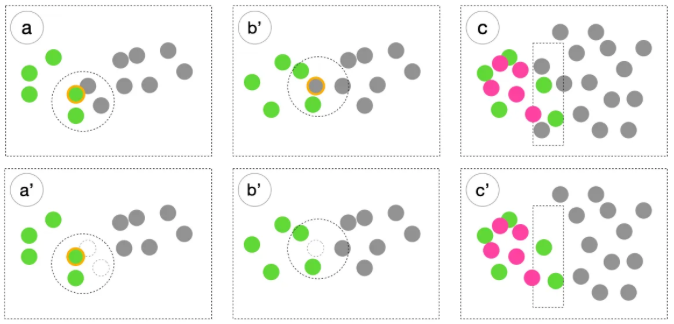
\includegraphics[width=0.9\textwidth]{images/SMOTE-EEN.png}
  \caption[Illustration of \gls{smote}-\acrshort{enn} Process]{Illustration of the \gls{smote}-\acrshort{enn} process, focusing on the \gls{enn} cleaning step. Panels (a) and (a') show an example where a minority sample's (green, highlighted) neighbors are examined, and in (a'), the sample is removed because its class label disagrees with the majority of its k-nearest neighbors. Panels (b) and (b') show a similar example for a majority sample (grey, highlighted) that is removed in (b') based on the same \gls{enn} rule. Panels (c) and (c') depict a dataset after \gls{smote} oversampling (original green/grey, synthetic pink) in (c'), samples inconsistent with their local neighborhood majority, as determined by the \gls{enn} rule, have been removed. This cleaning step helps to eliminate noise and ambiguous points, resulting in more clearly defined class boundaries. Figure adapted from figure 7 presented in \cite{Truong2022SMOTEVariants}.}
  \label{fig:SMOTE-ENN} % Corrected label spelling
\end{figure}
\\
\noindent
Similarly, \gls{smote}-\gls{enn} (\acrlong{enn}) \cite{Batista2004Study} is another hybrid technique that follows \gls{smote} oversampling with a cleaning step based on Wilson’s \acrlong{enn} (\gls{enn}) rules. In the \gls{enn} component, applied after the initial \gls{smote} oversampling, the dataset is cleaned based on the local neighborhood consistency of each sample $S_i$. For each sample $S_i$ (which can be original or synthetic), its \gls{kknn} are identified, and the ratio ($r$) of majority class instances among these \acrshort{kknn} is calculated. The \gls{enn} cleaning rule then applies as follows:
\begin{itemize}
    \item If a sample $S_i$ belongs to the minority class and the ratio $r$ of majority instances among its \acrshort{kknn} is greater than 0.5 ($r > 0.5$), then the majority instances among its \acrshort{kknn} are removed. This scenario is conceptually illustrated in Figure~\ref{fig:SMOTE-ENN}(a and a').
    \item If a sample $S_i$ belongs to the majority class and the ratio $r$ of majority instances among its \acrshort{kknn} is less than 0.5 ($r < 0.5$), then the sample $S_i$ itself is removed. This scenario is conceptually illustrated in Figure~\ref{fig:SMOTE-ENN}(b and b').
\end{itemize}
This rule is applied to aggressively clean the dataset by removing instances (original or synthetic) that appear to be mislabeled or that create ambiguity by being inconsistent with their local neighborhood's dominant class. The application of \gls{enn} cleaning after \gls{smote} oversampling results in the removal of inconsistent samples, leading to more clearly defined class clusters, as shown in Figure~\ref{fig:SMOTE-ENN}(c and c'). Compared to Tomek link removal, the \gls{enn} cleaning process typically removes more samples, potentially resulting in a more significant clarification of boundaries but also carrying a higher risk of removing potentially informative instances near the true decision boundary.\\
\\
By training separate models for each dataset using training data generated by each of these methods (including 'None' for no oversampling), the analysis allowed for a comprehensive exploration of the impact of different imbalance correction strategies on model performance and subsequent feature importance analysis.

\subsubsection*{Train and Evaluate Models \hyperref[fig:pipeline-2]{(G)}}
In this final stage of the pipeline, the various classification models outlined in Table~\ref{tab:ml_models} were trained and subsequently evaluated. For each dataset and each applied oversampling strategy (including the 'None' case), instances of these models were trained using the respective preprocessed training data partition ($n=32$). Following training, each model's performance was assessed on the untouched hold-out test set ($n=8$).\\
\\
Given the inherent class imbalance of the dataset, Balanced Accuracy was selected as the primary performance metric for evaluating the models in this study, providing a more robust measure than standard accuracy by accounting for the performance on both minority and majority classes. To complement the evaluation on the small test set, additional analyses related to model performance characteristics were conducted on the training data. Specifically, 95\% confidence intervals for the Balanced Accuracy were calculated based on a bootstrapping procedure applied to the training data. This bootstrapping technique, used for reasons related to limited data as discussed in Subsection~\ref{subsec:pipeline_structure_for_heterogeneous_datasets}, is illustrated and explained in detail in Figure~\ref{fig:Bootstrapping-1}.\\
\\
Furthermore, statistical significance was assessed using permutation tests applied to the training data. The permutation test technique, also used for reasons related to limited data as discussed in Subsection~\ref{subsec:pipeline_structure_for_heterogeneous_datasets}, is illustrated and explained in detail in Figure~\ref{fig:P-value_test-1}. This involved repeatedly permuting the true class labels of the training data and recalculating the Balanced Accuracy to determine the likelihood of achieving the observed training performance by chance.\\
\\
The Balanced Accuracy score, its 95\% bootstrapped confidence interval, and the p-value from the permutation test were computed for each trained model under every oversampling condition for each dataset. These performance parameters were then saved. these saved evaluation metrics served as the basis for the subsequent filtering and selection of "best" performing model configurations prior to the \gls{shap} analysis for feature importance identification.

\subsection{Feature Importance Assessment using \gls{shap}}
\label{subsec:shap-explanation}
% \todo{
% \begin{itemize}
%     \item \textbf{Introduction and Purpose:} Explain why feature importance is relevant and introduce SHAP as the chosen method, highlighting its advantages and what SHAP values represent.
%     \item \textbf{SHAP Calculation Details:} Describe which data instances were used for SHAP calculation and mention the specific SHAP explainer(s) employed.
% \end{itemize}
% }
\noindent
Knowing which factors contribute to a model's prediction is essential, especially in complex biological contexts where machine learning is used to uncover insights into underlying mechanisms. In this study, identifying the features that significantly influence the prediction of vaccine response is key to understanding the potential biological or clinical associations involved. The goal of feature importance techniques is to measure how much each input feature contributes to the model's output.\\
\\
To assess feature importance and provide interpretable explanations for the models, \gls{shap} \cite{ApprouchForModelPredictions} was used. \gls{shap} is a unified framework rooted in cooperative game theory, using Shapley values to assess the contribution of each feature to the difference between an individual prediction and the average prediction. Formally, the \gls{shap} value of a feature for a specific instance represents the average marginal contribution of that feature's value to the prediction, considering all possible combinations of features. A fundamental property of \gls{shap} values is their additivity, which provides a clear link between feature contributions and the model's output. For any given instance $x$, the \gls{shap} values ($\phi_i$) for all features $i=1, \dots, M$ sum up to the difference between the model's output for that instance, $f(x)$, and the expected base value (average output) over the dataset, $E[f(x)]$. This relationship can be formally expressed as:
$$ f(x) = E[f(x)] + \sum_{i=1}^M \phi_i $$
\noindent
Here, $E[f(x)]$ represents the base value of the prediction, which is typically the average prediction over the training data or a representative background dataset. The \gls{shap} value $\phi_i$ for feature $i$ quantifies the feature's contribution to pushing the prediction from this base value $E[f(x)]$ to the final output $f(x)$. A feature with a positive \gls{shap} value ($\phi_i > 0$) increases the model's output relative to the base value, while a negative \gls{shap} value ($\phi_i < 0$) decreases it, as illustrated in Figure~\ref{fig:SHAP-individual-explained}. For binary classification models, \gls{shap} values are typically on the log-odds scale.\\

% images based on https://shap.readthedocs.io/en/latest/example_notebooks/overviews/An%20introduction%20to%20explainable%20AI%20with%20Shapley%20values.html
\begin{figure}[h!]
  \centering
  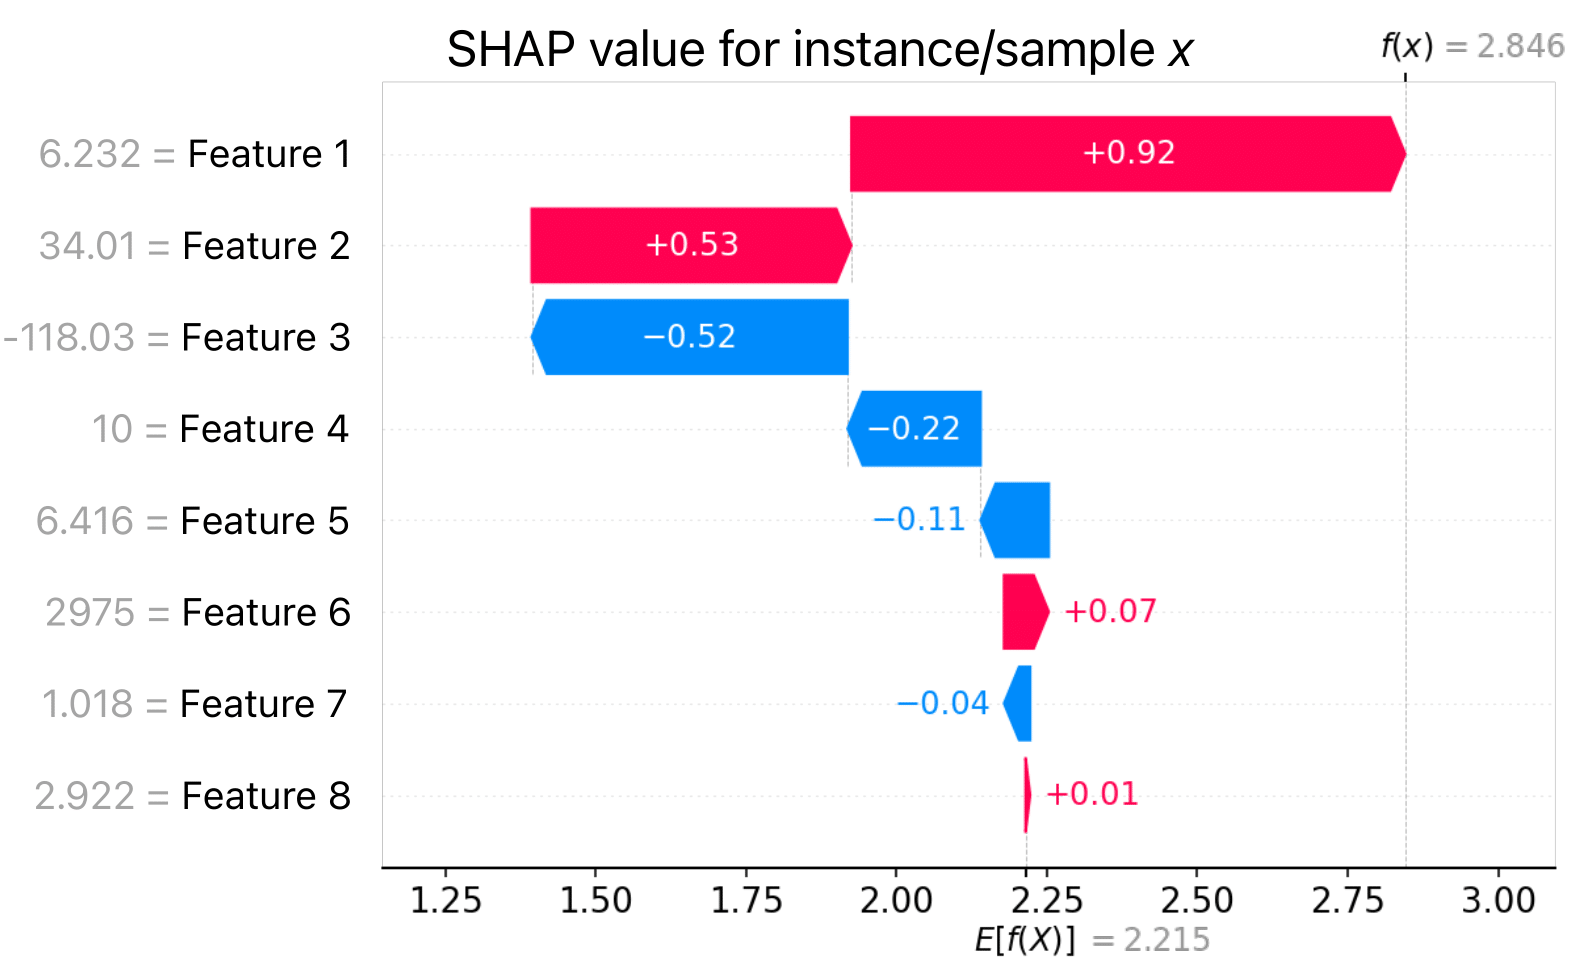
\includegraphics[width=0.9\textwidth]{images/SHAP-explained-individual.png}
  \caption[Example \gls{shap} Individual Explanation Plot]{An example \gls{shap} individual explanation plot for a single instance (sample x). This plot illustrates how each feature's value contributes to the model's prediction for this specific instance, moving from the expected base value ($E[f(x)] = 2.215$) to the final predicted output ($f(x) = 2.846$). Each arrow represents a feature's \gls{shap} value ($\phi_i$); red arrows indicate positive contributions that increase the output, while blue arrows indicate negative contributions that decrease the output. The width of each arrow corresponds to the magnitude of the feature's impact. Features are listed on the left along with their actual values for this instance.}
  \label{fig:SHAP-individual-explained} % Corrected label for clarity
\end{figure}
\noindent A common and informative visualization of \gls{shap} values across an entire dataset (or a representative subset) is the \gls{shap} summary plot, an example of which is shown in Figure~\ref{fig:SHAP-plot-explained}. This  plot is essentially an aggregation of the individual \gls{shap} explanation plots (like Figure~\ref{fig:SHAP-individual-explained}) for many instances and provides a rich overview of feature importance and the relationship between feature values and their impact on model predictions. Interpreting the \gls{shap} summary plot involves understanding its key components:
\pagebreak
\begin{itemize}
    \item \textbf{Y-axis:} Features are listed on the vertical axis, ordered by their overall importance from top to bottom. A feature's overall importance is typically measured by the average of the absolute \gls{shap} values for that feature across all instances in the plot. Features higher on the list have a greater average impact on the magnitude of the model's output difference from the average prediction.
    \item \textbf{X-axis:} The horizontal axis represents the \gls{shap} value ($\phi_i$) (impact on model output). For a binary classification model trained to predict Label 1 (the positive class) versus Label 0 (the negative class), positive \gls{shap} values ($>0$) indicate that the feature's value increases the model's output, pushing the prediction towards the positive class (Label 1). Conversely, negative \gls{shap} values ($<0$) indicate that the feature's value decreases the model's output, pushing the prediction towards the negative class (Label 0). The position of a point along the x-axis shows the magnitude and direction of a specific feature's impact for a particular instance.
    \item \textbf{Color:} Each point on the plot is colored according to the actual value of the feature it represents for that specific data instance. The color bar shown on the right (as in Figure~\ref{fig:SHAP-plot-explained}), maps the color to the feature value scale (e.g., red indicates a high feature value, and blue indicates a low feature value). This allows for examining how the value of a feature relates to the direction and magnitude of its impact.
    \item \textbf{Each point:} Represents the \gls{shap} value ($\phi_i$) for a single data instance. For each feature (row on the y-axis), the plot displays a distribution of points along the x-axis. The horizontal spread and density of points for a single feature illustrate the variability in its impact across different data points.
\end{itemize}
\begin{figure}[h!]
  \centering
  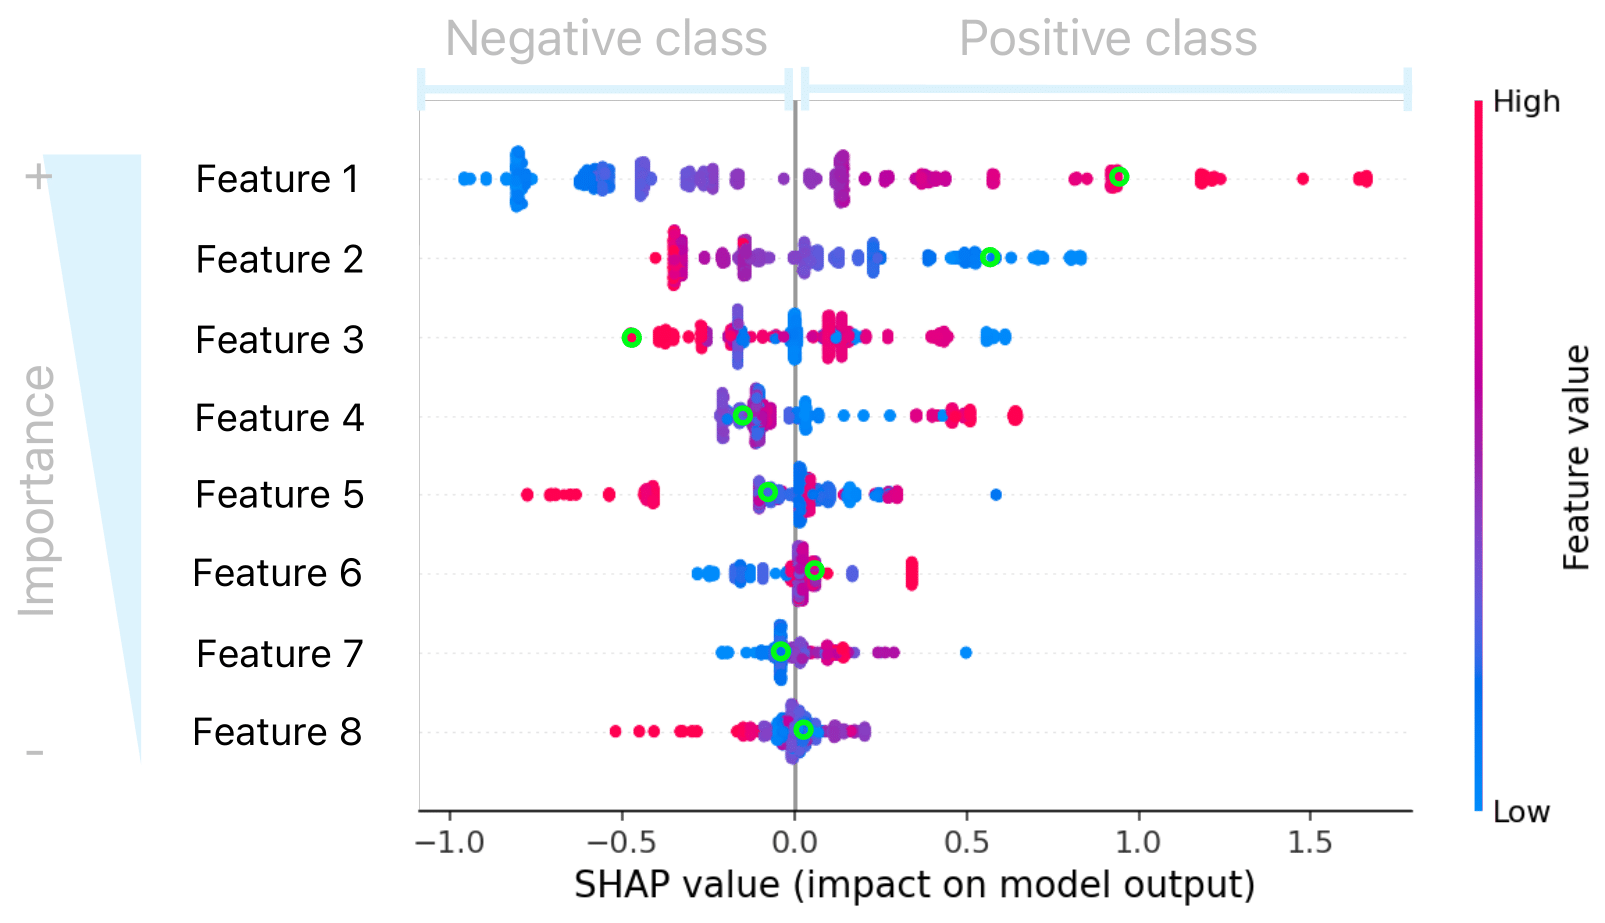
\includegraphics[width=0.9\textwidth]{images/SHAP-explained.png}
  \caption[Example \gls{shap} Summary Plot]{An example \gls{shap} summary plot. This visualization shows the overall importance of features and how their values impact the model's output across a dataset. Features are ranked by importance on the y-axis, the x-axis represents the impact (\gls{shap} value), and the color indicates the feature value (low to high). Points on the left push the prediction towards the negative class, while points on the right push it towards the positive class. Points corresponding to the \gls{shap} values from an individual explanation (as shown in Figure~\ref{fig:SHAP-individual-explained}) are highlighted in green for context.}
  \label{fig:SHAP-plot-explained}
\end{figure}
\noindent
Calculating exact Shapley values is computationally intensive for most models. Therefore, estimation methods are used to approximate them. KernelSHAP \cite{ApprouchForModelPredictions} is model-agnostic, so the approach is designed to estimate \gls{shap} values for any type of machine learning model. It approximates the Shapley values by fitting a weighted linear regression model. The process involves sampling numerous coalitions of features, where a coalition is simply a subset of the original features. For each sampled coalition, a corresponding data instance is created (typically by using the feature values from the instance being explained for features in the coalition, and replacing the values of absent features with values from a background dataset). The original machine learning model then makes a prediction for each of these created instances. These predictions serve as the target variable in a linear regression model, where the input features are binary indicators representing whether each original feature was present in the coalition. This regression is weighted using the \gls{shap} kernel, which is designed to give specific weights to different coalition sizes to ensure that the coefficients of the linear model approximate the Shapley values. The coefficients ($\beta_i$) of this fitted weighted linear model are the estimated \gls{shap} values ($\phi_i$). While general and theoretically connected to Shapley values, KernelSHAP can be computationally slow due to the sampling and regression steps.\\
\\
In contrast to model-agnostic methods, TreeSHAP \cite{Lundberg2019TreeSHAP} is a \gls{shap} variant specifically optimized for tree-based machine learning models, including Decision Trees and Random Forest models. TreeSHAP significantly reduces the computational complexity compared to general methods like KernelSHAP by efficiently leveraging the inherent structure of decision trees to compute \gls{shap} values. For individual decision trees, TreeSHAP can compute exact \gls{shap} values (or very good approximations) much faster than KernelSHAP. For ensembles of trees, such as Random Forests, the final \gls{shap} value for a feature is typically the average of the \gls{shap} values computed for that feature in each individual tree in the ensemble. TreeSHAP provides a much more efficient approach for interpreting this important class of models.\\
\\
The \gls{shap} values for the respective models were estimated using the implementations available in the \texttt{shap} Python library. Specifically, \texttt{shap.KernelExplainer} was utilized for the non-tree-based models (Logistic Regression, Support Vector Machine, Gaussian Naive Bayes), and \texttt{shap.TreeExplainer} was used for the tree-based models (Random Forest, Decision Tree). These explainers interact with the scikit-learn model objects to compute the \gls{shap} values.\\
\\
By examining the distribution of points for each feature, their spread along the x-axis and their corresponding colors, one can infer detailed insights into the model's behavior. For instance, if for a feature, points that are red (high feature value) tend to cluster on the right side (positive \gls{shap} values), it suggests that higher values of that feature increase the model's output and thus increase the predicted probability (or log-odds) of the positive class (Label 1). Conversely, if blue points (low feature value) are predominantly on the left side (negative \gls{shap} values), it indicates that lower values of that feature decrease the model's output, pushing the prediction towards the negative class (Label 0). The \gls{shap} summary plot thus serves as a powerful tool for understanding global feature importance and their directional relationships with the prediction outcome.

\subsection{Aggregation of \gls{shap} Values for Global Importance}
% \todo{
% \begin{itemize}
%     \item \textbf{Rationale for Using SHAP Across Multiple Models:} Explain the reasoning behind using SHAP on multiple models (e.g., robustness) rather than a single model.
% \end{itemize}
% }
While \gls{shap} is capable of providing global feature importance for a single model, identifying features that are truly and robustly influential across different modeling approaches is crucial in this study. Due to the inherent limitations of the dataset, including its relatively small size and potential complexity, individual models trained under various conditions might not achieve consistently high or "perfect" accuracy. In such scenarios, relying solely on the global feature importance derived from a single model could potentially lead to conclusions that are overly specific to that model or the particular data balancing strategy used.\\
\\
Therefore, to obtain a more robust and generalizable assessment of feature importance, a strategy was adopted that involved calculating and aggregating \gls{shap} values across a selection of models trained with diverse algorithms and various \gls{smote}-based oversampling techniques. By analyzing the \gls{shap} explanations from multiple models that demonstrated promising performance on the evaluation criteria outlined in Subsection~\ref{subsec:pipeline_structure_for_heterogeneous_datasets} (referencing the model evaluation step), the aim was to find consensus among these models regarding which features were most influential. This aggregation strategy enables a more robust assessment of feature importance by identifying features with consistent impact across models and data preparation methods, suggesting stable associations with vaccine response.\\
\\
For each individual model included in the analysis, the overall importance of each feature within that model was first quantified by calculating the mean absolute \gls{shap} value for that feature across all the explained instances for that model. These per-model mean absolute \gls{shap} values were then normalized. This normalization step was performed to ensure that each model contributed approximately equally to the subsequent aggregation, preventing models with generally larger or smaller \gls{shap} value scales from dominating the combined importance ranking.\\
\\
To derive a single, aggregated measure of importance for each feature across all the selected models, the normalized mean absolute \gls{shap} values for that feature were collected from every model in which it was present. The median of these per-model normalized mean absolute \gls{shap} values was then calculated for each feature. Using the median helps to reduce the influence of potentially extreme importance scores from any single model or noise. Features were subsequently ranked in descending order based on these calculated median aggregated normalized mean absolute \gls{shap} values, which determined their vertical order in the combined summary plot, as illustrated in Appendix~\ref{appendix:shap_aggregation}, Figure~\ref{fig:SHAP-aggregate-explained}.

\subsection{Limitations of \gls{smote}-\gls{enn}}
\noindent
While various oversampling and undersampling techniques were explored to address the class imbalance inherent in the dataset, the \gls{smote}-\gls{enn} method was ultimately excluded from the set of techniques used for the final model training and selection. This decision was based on observations during preliminary model evaluation and data visualization, which indicated that \gls{smote}-\gls{enn} exhibits an overly aggressive sampling behavior that can significantly distort the original data distribution.\\
\\
\gls{smote}-\gls{enn} combines the \acrfull{smote}, which generates synthetic samples for the minority class, with \acrfull{enn}, a technique that removes samples (both synthetic and original) considered "noisy" if their class label differs from the majority of their neighbors as seen in Figure~\ref{fig:SMOTE-ENN}. In practice, particularly with potentially noisy biological data, this combined approach was found to be excessively aggressive. It led to the generation of a significant number of synthetic samples while simultaneously removing a substantial portion of the original data points from the training set. This process resulted in training datasets that were not representative of the true underlying data distribution, potentially introducing bias and hindering the model's ability to generalize to unseen data.\\
\\
The consequence of this aggressive resampling was observed in the inconsistent and often unreliable performance of models trained with \gls{smote}-\gls{enn} on the unseen test set. Despite achieving seemingly good performance on the modified training data (as indicated by cross-validation scores), the models' performance on the original, unmodified test set varied significantly. Sometimes appearing high potentially due to chance or overfitting to the distorted training distribution, and other times being very poor. This unpredictability raised concerns about the reliability of any model trained using this method for downstream interpretation.\\
\begin{figure}[h!]
    \centering

    % First row of subfigures (e.g., a & b)
    \begin{subfigure}[b]{0.48\textwidth}
        \centering
        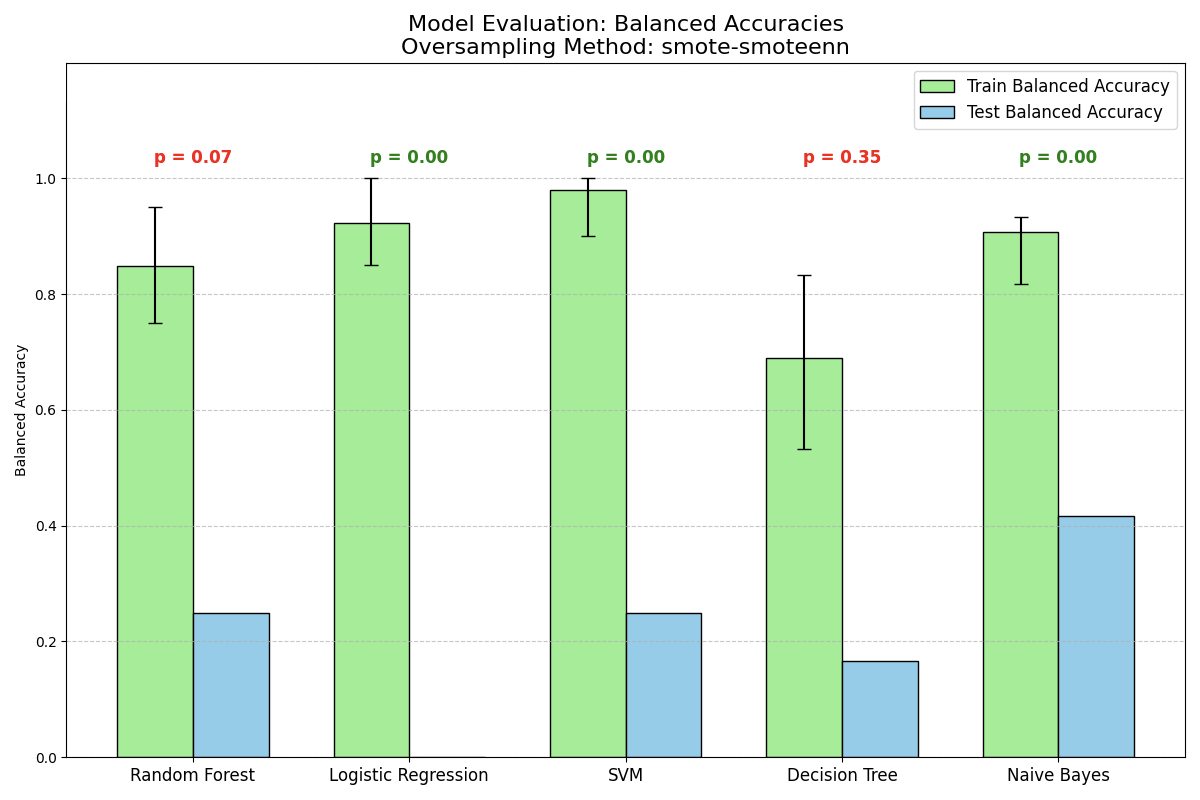
\includegraphics[width=\textwidth]{images/smote_een_fig1a.png}
        \caption{Balanced Accuracy Scores}
        \label{fig:smote_enn_fig1a}
    \end{subfigure}
    \hfill
    \begin{subfigure}[b]{0.48\textwidth}
        \centering
        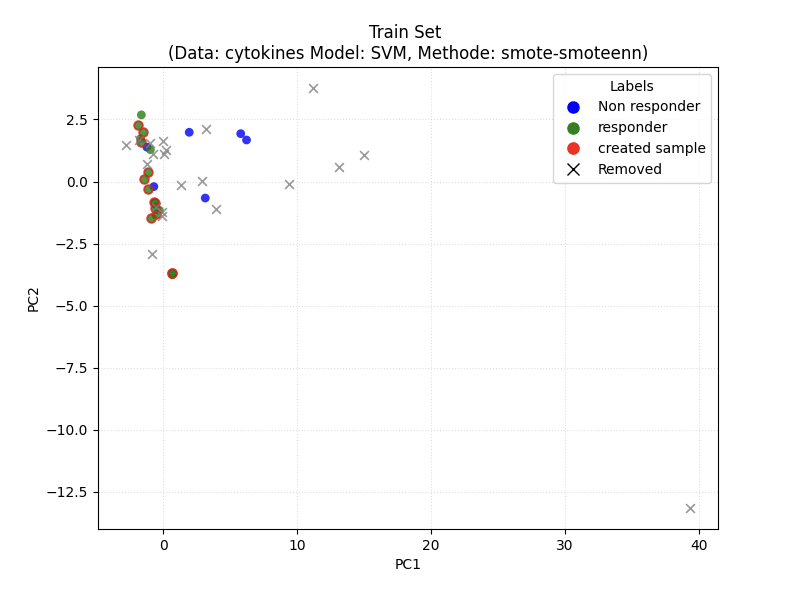
\includegraphics[width=0.9\linewidth]{images/smote_een_fig1b.png}
        \caption{\gls{pca} Visualization of Training Data}
        \label{fig:smote_enn_fig1b}
    \end{subfigure}

    \vspace{1em}

    % Second row of subfigures (e.g., c & d)
    \begin{subfigure}[b]{0.48\textwidth}
        \centering
        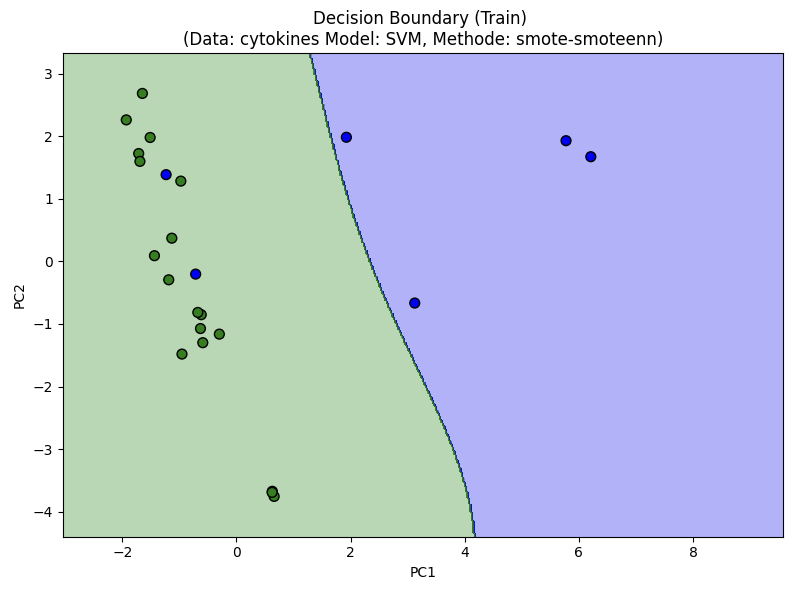
\includegraphics[width=\textwidth]{images/smote_een_fig1c.png}
        \caption{Decision Boundary with train set samples}
        \label{fig:smote_enn_fig1c}
    \end{subfigure}
    \hfill
    \begin{subfigure}[b]{0.48\textwidth}
        \centering
        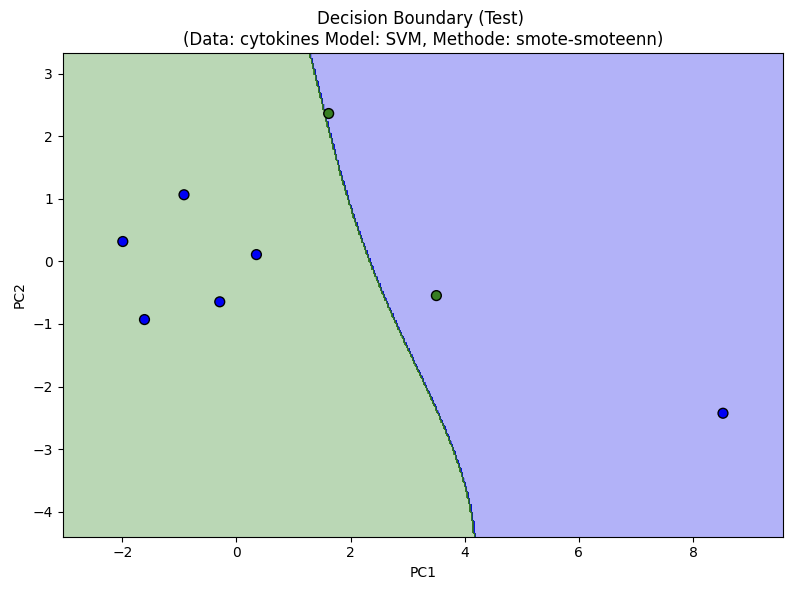
\includegraphics[width=\textwidth]{images/smote_een_fig1d.png}
        \caption{Decision Boundary with test set samples}
        \label{fig:smote_enn_fig1d}
    \end{subfigure}

    \caption[Visualizing \gls{smote}-\gls{enn} on Cytokines]{Visualizing the aggressive sampling behavior of \gls{smote}-\gls{enn} and its effect on model learning using the Cytokines dataset. (a) Balanced Accuracy scores on train and test sets for models trained with \gls{smote}-\gls{enn}. (b) \gls{pca} visualization of the training data distribution after \gls{smote}-\gls{enn} application, highlighting synthetic and removed original samples. (c, d) Examples of decision boundaries learned by representative models trained on this distorted data in the \gls{pca} space.}
    \label{fig:smote-enn-example-1}
\end{figure}


\begin{figure}[h!]
    \centering

    % First row of subfigures (e.g., a & b)
    \begin{subfigure}[b]{0.48\textwidth}
        \centering
        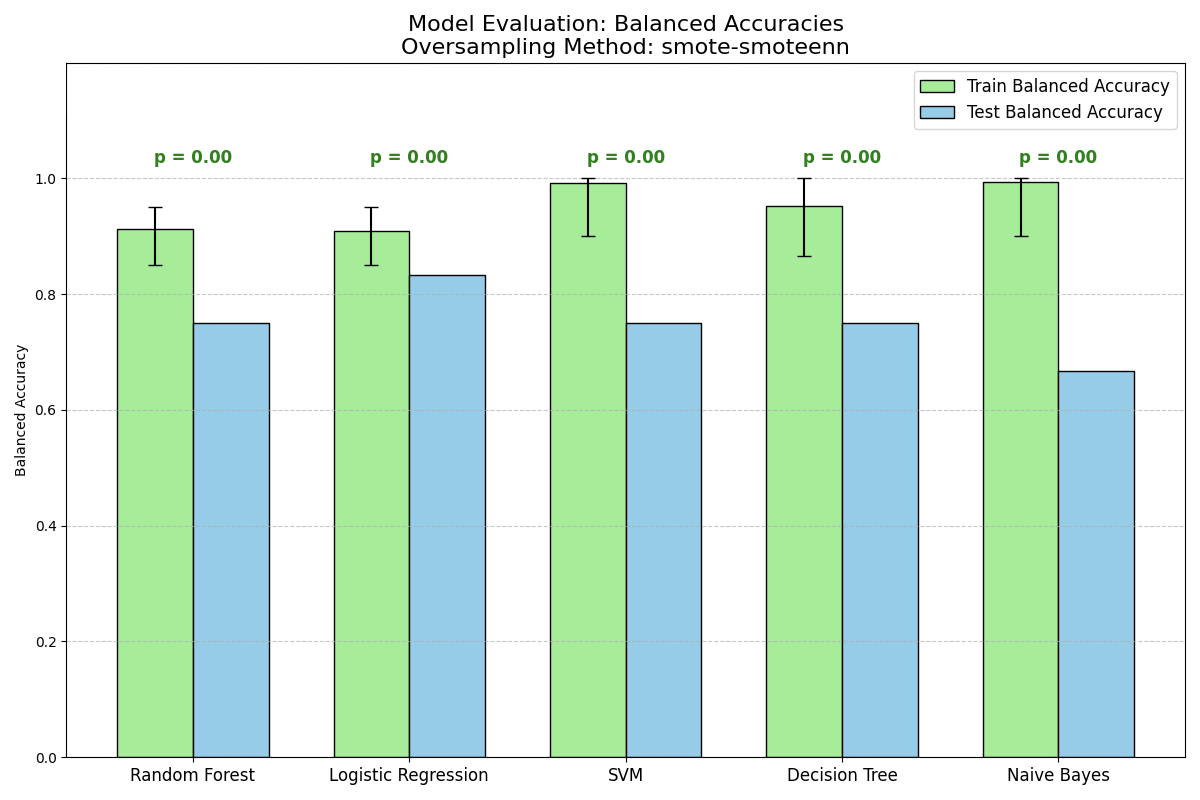
\includegraphics[width=\textwidth]{images/smote_een_fig2a.png}
        \caption{Balanced Accuracy Scores}
        \label{fig:smote_enn_fig2a}
    \end{subfigure}
    \hfill
    \begin{subfigure}[b]{0.48\textwidth}
        \centering
        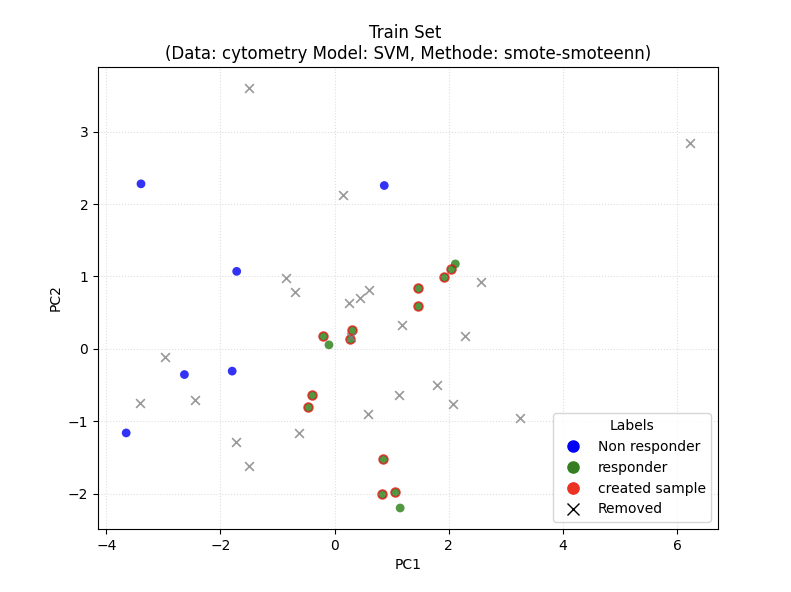
\includegraphics[width=0.9\textwidth]{images/smote_een_fig2b.png}
        \caption{\gls{pca} Visualization of Training Data}
        \label{fig:smote_enn_fig2b}
    \end{subfigure}

    \vspace{1em}

    % Second row of subfigures (e.g., c & d)
    \begin{subfigure}[b]{0.48\textwidth}
        \centering
        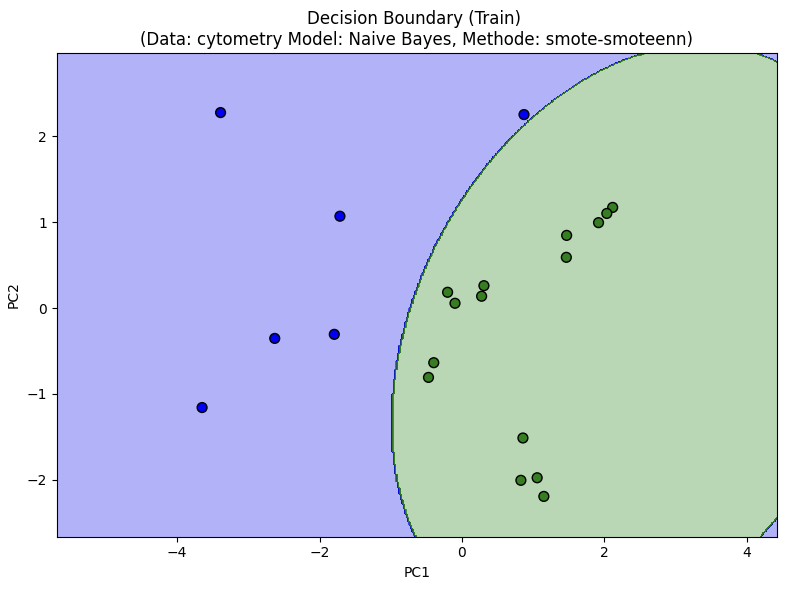
\includegraphics[width=\textwidth]{images/smote_een_fig2c.png}
        \caption{Decision Boundary with train set samples}
        \label{fig:smote_enn_fig2c}
    \end{subfigure}
    \hfill
    \begin{subfigure}[b]{0.48\textwidth}
        \centering
        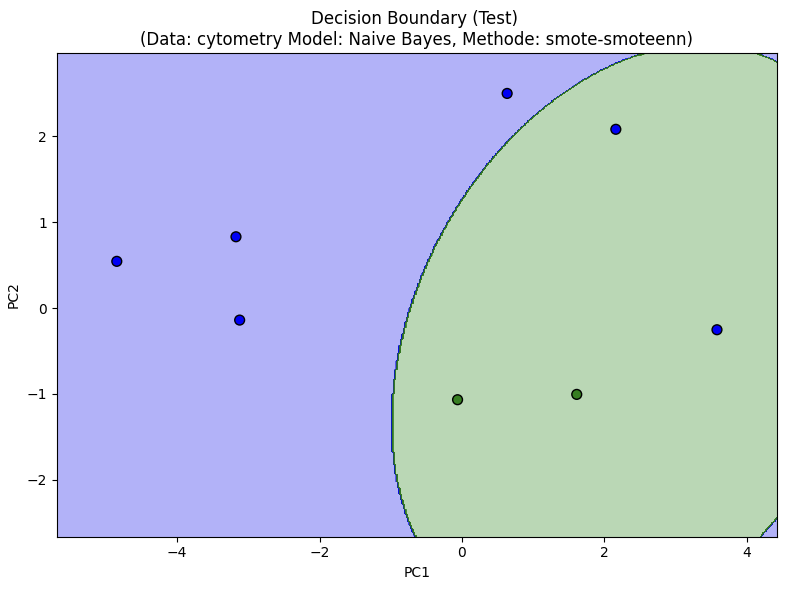
\includegraphics[width=\textwidth]{images/smote_een_fig2d.png}
        \caption{Decision Boundary with test set samples}
        \label{fig:smote_enn_fig2d}
    \end{subfigure}


    \caption[Visualizing \gls{smote}-\gls{enn} on Cytometry]{Visualizing the aggressive sampling behavior of \gls{smote}-\gls{enn} and its effect on model learning using the Cytometry dataset. (a) Balanced Accuracy scores on train and test sets for models trained with \gls{smote}-\gls{enn}. (b) \gls{pca} visualization of the training data distribution after \gls{smote}-\gls{enn} application, highlighting synthetic and removed original samples and showing the severe reduction in original minority samples. (c, d) Examples of decision boundaries learned by representative models trained on this distorted data in the \gls{pca} space.}

    \label{fig:smote-enn-example-2}
\end{figure}

\noindent
To visually demonstrate the impact of \gls{smote}-\gls{enn}'s aggressive sampling on the data distribution, \acrfull{pca} was utilized for dimensionality reduction, projecting the training data into a 2-dimensional space. Figure~\ref{fig:smote-enn-example-1} illustrates the effect of applying \gls{smote}-\gls{enn} to the Cytokines dataset. Figure~\ref{fig:smote-enn-example-1}a shows a summary of Balanced Accuracy scores on the training and test sets for various models trained with \gls{smote}-\gls{enn}. Figure~\ref{fig:smote-enn-example-1}b visualizes the \gls{pca}-reduced training space after \gls{smote}-\gls{enn} application for a representative model (e.g., an SVM, chosen for visualization clarity), highlighting the synthetic samples generated by \gls{smote} (e.g., circled in red) and the original samples that were removed by the \gls{enn} step (e.g., marked with a cross). Figures~\ref{fig:smote-enn-example-1}c and \ref{fig:smote-enn-example-1}d further show the decision boundary learned by the representative model form the distorted data distribution in the \gls{pca} space, illustrating what the model is learning from this modified data.\\
\\
A similar visualization was performed for the Cytometry dataset (Figure~\ref{fig:smote-enn-example-2}), using a different representative model (e.g., a Naive Bayes classifier, also chosen for visualization clarity). Figure~\ref{fig:smote-enn-example-2}a presents the Balanced Accuracy scores for models trained with \gls{smote}-\gls{enn} on this dataset. Figure~\ref{fig:smote-enn-example-2}b visualizes the \gls{pca}-reduced training space, clearly showing the generated synthetic samples and the removed original samples. In the case of the Cytometry dataset with \gls{smote}-\gls{enn}, it was observed that the training set for the minority class contained very few original samples, with the vast majority being synthetic. This severe distortion of the original data distribution made it questionable whether any model trained on such a set could reliably capture the true underlying patterns relevant to predicting outcomes on real, unseen data, even if it happened to score well on the small test set (potentially due to chance or severe overfitting).\\
\\
Based on this visual evidence of aggressive data manipulation and the resulting concerns regarding the representativeness of the training data and the reliability of model performance, \gls{smote}-\gls{enn} was excluded from the set of oversampling methods used for the final model selection and subsequent interpretation via SHAP values. Only models trained with less aggressive and more reliable data handling techniques were considered for the main analysis to ensure that the insights derived were based on models that learned from a representative data distribution.

\pagebreak
\subsection{Interpretation and Conclusion of Feature Identification}
\label{subsec:feature_identification}

\noindent
Having established the methodology for assessing model interpretability using \gls{shap} values (Section~\ref{subsec:shap-explanation}) and addressed data imbalance through various oversampling techniques (Section~\ref{subsec:pipeline_structure_for_Heterogeneous_datasets}, Up-sample Train set (E)), this section presents the results of the \gls{shap} analysis for the selected models for each dataset, aimed at identifying the key features that contribute most to the measles vaccine response prediction.\\
\\
The selection of models deemed most suitable for the feature importance analysis using aggregated \gls{shap} values was based on their performance on the unseen test set and the statistical significance of their performance on the training data. Considering the limited size of the test set, reliance solely on test set metrics could be misleading and prone to chance findings. Therefore, models were chosen based on the following criteria:
\begin{itemize}
    \item The model's Test Balanced Accuracy must be $\geq 0.5$, indicating performance at least equivalent to random chance on the imbalanced test set (where 0.5 represents the baseline Balanced Accuracy achieved by simply predicting the majority class).
    \item The model's training performance, assessed via a permutation test on the training data, must have a p-value $< 0.05$, providing statistical evidence that the model learned meaningful patterns on the training data beyond what would be expected by chance.
    \item Additionally, to ensure adequate predictive capability for both responder and non-responder classes, the model's Classification Report metrics (Recall and Precision) for each class on the test set must meet specific thresholds, aiming for performance at or above the 50/50 random baseline:
    \begin{itemize}
        \item Recall for Class 0 (Non-responders) must be $\geq 0.5$.
        \item Precision for Class 0 (Non-responders) must be $\geq 0.5$.
        \item Recall for Class 1 (Responders) must be $\geq 0.5$.
        \item Precision for Class 1 (Responders) must be $\geq 0.5$.
    \end{itemize}
\end{itemize}
Only models satisfying all of these criteria were deemed sufficiently robust and reliable to be included in the aggregated \gls{shap} analysis.
\subsubsection*{Cytokines Dataset Results}

For the Cytokines dataset, applying the selection criteria resulted in the following models being chosen for aggregated \gls{shap} analysis (see Table~\ref{tab:cytokines_selected_models}):

\begin{table}[H]
    \centering
    \scalebox{0.85}{
    \begin{tabular}{l l l l l l}
        \toprule
        Model & Oversampling & Test Bal. Acc. & Train $p$-val & Train Bal. Acc. ($\mu$/Md) \\
        \midrule
        Logistic Regression & smote & 0.625 & 0.007 & 0.74246 \ \ \ / \ \ \ 0.74000 \\
        Logistic Regression & smote-borderline & 0.007 & 0.016 & 0.74414 \ \ \ / \ \ \ 0.74000 \\
        Logistic Regression & smote-adasyn & 0.750 & 0.005 & 0.74562 \ \ \ / \ \ \ 0.74000 \\
        Logistic Regression & smote-smotetomek & 0.625 & 0.028 & 0.72932 \ \ \ / \ \ \ 0.73000 \\
        \bottomrule
    \end{tabular}}
    \caption[Selected Models for Cytokines]{Models selected for aggregated SHAP analysis for the Cytokines dataset.}
    \label{tab:cytokines_selected_models}
\end{table}
\begin{figure}[h!]
    \centering
    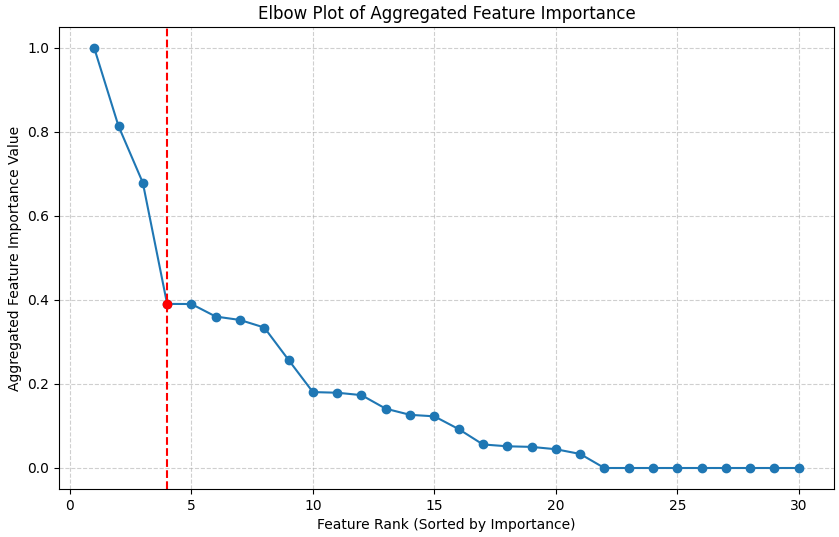
\includegraphics[width=0.9\textwidth]{images/elbow_plot_cytokines_uncompressed.png}
    \caption[Elbow plot for Cytokines]{Elbow plot showing the ranked trajectory of aggregated \gls{shap} values for the Cytokines dataset. These values are identical to those visualized in the aggregated SHAP summary plot in Figure~\ref{fig:cytokines_aggregated_shap}, and are used here to determine a feature selection cutoff point.}
    \label{fig:elbow_plot_cytokines_uncompressed}
\end{figure}
\begin{figure}[h!]
    \centering
    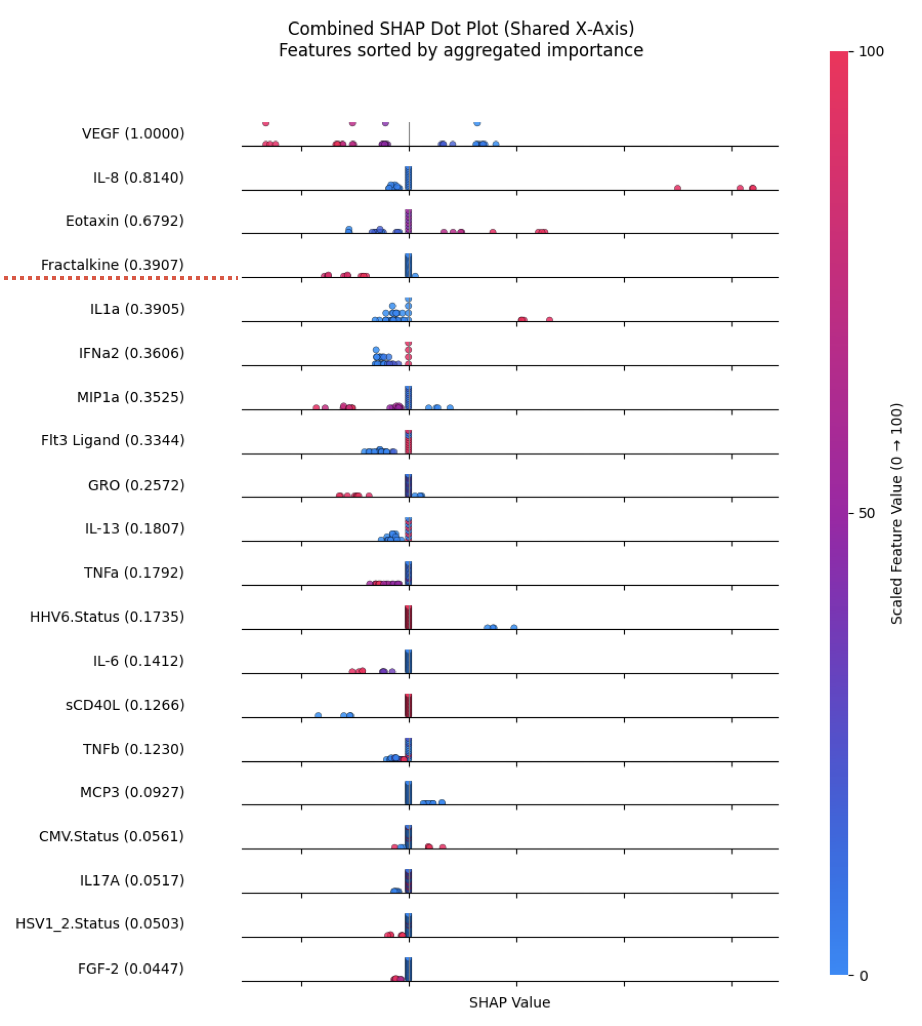
\includegraphics[width=0.9\linewidth]{images/Aggregated_SHAP_cytokines_uncompressed.png}
    \caption[Aggregated SHAP plot for Cytokines]{Aggregated SHAP summary plot for the Cytokines dataset.}
    \label{fig:cytokines_aggregated_shap}
\end{figure}


\noindent
Given the number of features in the dataset, identifying a clear numerical threshold for feature importance can be challenging, as importance is relative and context-dependent. Therefore, the elbow method, commonly used in contexts like clustering (e.g., to determine the optimal number of clusters) or Principal Component Analysis (e.g., to select the number of components based on explained variance), was employed as a data-driven approach to help distinguish features with a more substantial impact from those with diminishing returns in importance.\\
\\
This method involves plotting aggregated feature importance values (in this case, \gls{shap} values) in descending order and identifying the point where the rate of decline changes most sharply, the "elbow." This point serves as a natural cutoff, separating key features from those with minimal added value. To identify the elbow point objectively, the \texttt{KneeLocator} function from the \texttt{kneed} Python package was used, as illustrated in Figure~\ref{fig:elbow_plot_cytokines_uncompressed}.\\
\\
Figure~\ref{fig:cytokines_aggregated_shap} presents the aggregated \gls{shap} summary plot for the Cytokines dataset, with features sorted by their aggregated importance. Based on the elbow method applied to these importance values (indicated visually by the dotted line in Figure~\ref{fig:cytokines_aggregated_shap}), the features identified as most influential for predicting vaccine response are those ranked above the elbow point. These features are: VEGF (1.000), IL-8 (0.8140), Eotaxin (0.6792) and Fractalkine (0.3907).\\
\\
Examining the aggregated \gls{shap} plot for these top features reveals patterns in how their values influence model output. For features like IL-8 and Eotaxin, higher feature values (red points) are linked to positive \gls{shap} values, pushing predictions toward the positive class, while lower values (blue points) are often linked to neutral or negative SHAP values, contributing less or pushing predictions toward the negative class. In contrast, features like VEGF and Fractalkine show the opposite trend: higher feature values are associated with negative \gls{shap} values, steering the model toward the negative class, and lower feature values push it toward the positive class.

\subsubsection*{Cytometry Dataset Results}
For the Cytometry dataset, applying the same selection criteria resulted in the following models being chosen for aggregated \gls{shap} analysis (see Table~\ref{tab:cytometry_selected_models_uncompressed}):\\

\begin{table}[H]
    \centering
    \scalebox{0.85}{
    \begin{tabular}{l l l l l}
        \toprule
        Model & Oversampling & Test Bal. Acc. & Train $p$-val & Train Bal. Acc. ($\mu$/Md) \\
        \midrule

        Random Forest       & smote & 0.750 & 0.000 & 0.815140 \ \ \ / \ \ \ 0.820000 \\
        Logistic Regression & smote & 0.625 & 0.002 & 0.673100 \ \ \ / \ \ \ 0.680000 \\
        SVM                 & smote & 0.625 & 0.000 & 0.838920 \ \ \ / \ \ \ 0.840000 \\
        Naive Bayes         & smote & 0.625 & 0.000 & 0.862480 \ \ \ / \ \ \ 0.860000 \\

        Random Forest       & smote-borderline & 0.750 & 0.000 & 0.816960 \ \ \ / \ \ \ 0.820000 \\
        Logistic Regression & smote-borderline & 0.625 & 0.002 & 0.674820 \ \ \ / \ \ \ 0.680000 \\
        SVM                 & smote-borderline & 0.625 & 0.000 & 0.837080 \ \ \ / \ \ \ 0.840000 \\
        Naive Bayes         & smote-borderline & 0.625 & 0.000 & 0.861980 \ \ \ / \ \ \ 0.860000 \\

        Random Forest       & smote-adasyn & 0.750 & 0.003 & 0.807230 \ \ \ / \ \ \ 0.803333 \\
        Logistic Regression & smote-adasyn & 0.625 & 0.008 & 0.708343 \ \ \ / \ \ \ 0.706667 \\
        SVM                 & smote-adasyn & 0.625 & 0.001 & 0.789600 \ \ \ / \ \ \ 0.800000 \\
        Decision Tree       & smote-adasyn & 0.500 & 0.001 & 0.797597 \ \ \ / \ \ \ 0.800000 \\
        Naive Bayes         & smote-adasyn & 0.625 & 0.000 & 0.850100 \ \ \ / \ \ \ 0.860000 \\

        Random Forest       & smote-smotetomek & 0.750 & 0.000 & 0.798965 \ \ \ / \ \ \ 0.800000 \\
        Logistic Regression & smote-smotetomek & 0.625 & 0.018 & 0.653180 \ \ \ / \ \ \ 0.655000 \\
        SVM                 & smote-smotetomek & 0.625 & 0.000 & 0.813845 \ \ \ / \ \ \ 0.815000 \\
        Naive Bayes         & smote-smotetomek & 0.625 & 0.000 & 0.848645 \ \ \ / \ \ \ 0.850000 \\
        \bottomrule
    \end{tabular}
    }
    \caption[Selected Models for Cytometry ]{Models selected for aggregated SHAP analysis for the Cytometry dataset.}
    \label{tab:cytometry_selected_models_uncompressed}
\end{table}
\begin{figure}[h!]
    \centering
    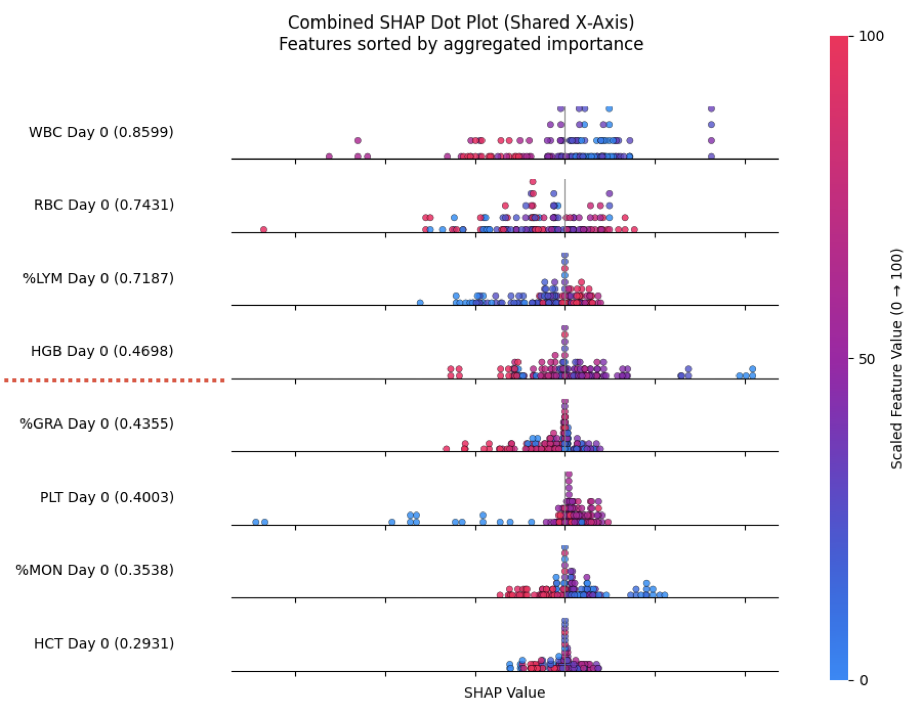
\includegraphics[width=0.9\linewidth]{images/Aggregated_SHAP_cytometry_uncompressed.png}
    \caption[Aggregated SHAP plot for Cytometry]{Aggregated \gls{shap} summary plot for the Cytometry dataset. The same SHAP values are used in the elbow plot shown in Appendix~\ref{appendix:elbow_plots}, Figure~\ref{fig:elbow_plot_cytomery_uncompressed}, where the cutoff is visualised.}
    \label{fig:cytometry_aggregated_shap}
\end{figure}

\noindent
Figure~\ref{fig:cytometry_aggregated_shap} illustrates the ranked importance of features based on their aggregated \gls{shap} values for the Cytometry dataset. At the forefront of importance is \gls{wbc}, with an aggregated importance score of 0.8599. The \gls{shap} value distribution for \gls{wbc} reveals a clear pattern: higher \gls{wbc} values (indicated by red points) correspond to negative \gls{shap} values, pushing the model's prediction towards the negative class (e.g., non-responder), while lower \gls{wbc} values (blue points) correspond to positive \gls{shap} values, pushing the model's prediction towards the positive class (e.g., responder).\\
\\
This inverse trend, where higher feature values push towards the negative class and lower values push towards the positive class, is also visible for \%\acrshort{gra} (Granulocytes percentage). Although \%\acrshort{gra} was not selected as one of the primary influential features by the elbow method, its consistent pattern makes it an interesting observation.\\
\\
In contrast,\%\acrshort{lym} (Lymphocyte percentage), with an importance of 0.7187, exhibits a direct relationship. Here, higher \%\acrshort{lym} values contribute positively to the model's output (positive \gls{shap} values), while lower values reduce it (negative \gls{shap} values). This suggests that higher lymphocyte percentages are predictive of a stronger modeled vaccine response.\\
\\
Based on the elbow method, the most influential features for predicting vaccine response from the Cytometry dataset are: \gls{wbc} (0.8599), \acrshort{rbc} (0.7431), \%\acrshort{lym} (0.7187), and \acrshort{hgb} (0.4698). While the specific \gls{shap} value distributions for \acrshort{rbc} and \acrshort{hgb} are not explicitly detailed, their inclusion based on the elbow method highlights their overall importance in the model's predictive framework.

\subsubsection*{\acrshort{rna} Dataset Results}
\noindent
For the \acrshort{rna} dataset, which comprises 382 features, the application of the selection criteria resulted in the models listed in Table~\ref{tab:rna_selected_models} being chosen for aggregated \gls{shap} analysis.

\begin{table}[H]
    \centering
    \scalebox{0.85}{
    \begin{tabular}{l l l l l}
        \toprule
        Model & Oversampling & Test Bal. Acc. & Train $p$-val & Train Bal. Acc. ($\mu$/Md) \\
        \midrule

        Logistic Regression & smote & 0.500 & 0.000 & 0.833840 \ \ \ / \ \ \ 0.84000 \\
        SVM                 & smote & 0.625 & 0.000 & 0.823600 \ \ \ / \ \ \ 0.82000 \\

        Logistic Regression & smote-borderline & 0.500 & 0.000 & 0.832860 \ \ \ / \ \ \ 0.84000 \\
        SVM                 & smote-borderline & 0.625 & 0.000 & 0.824820 \ \ \ / \ \ \ 0.82000 \\

        Logistic Regression & smote-adasyn & 0.500 & 0.000 & 0.830560 \ \ \ / \ \ \ 0.84000 \\
        SVM                 & smote-adasyn & 0.625 & 0.000 & 0.805060 \ \ \ / \ \ \ 0.80000 \\

        Logistic Regression & smote-smotetomek & 0.500 & 0.000 & 0.833280 \ \ \ / \ \ \ 0.84000 \\
        SVM                 & smote-smotetomek & 0.625 & 0.000 & 0.824700 \ \ \ / \ \ \ 0.82000 \\

        \bottomrule
    \end{tabular}
    }
    \caption[Selected Models for \acrshort{rna}]{Models selected for aggregated SHAP analysis for the \acrshort{rna} dataset.}
    \label{tab:rna_selected_models}
\end{table}
\begin{figure}[h!]
    \centering
    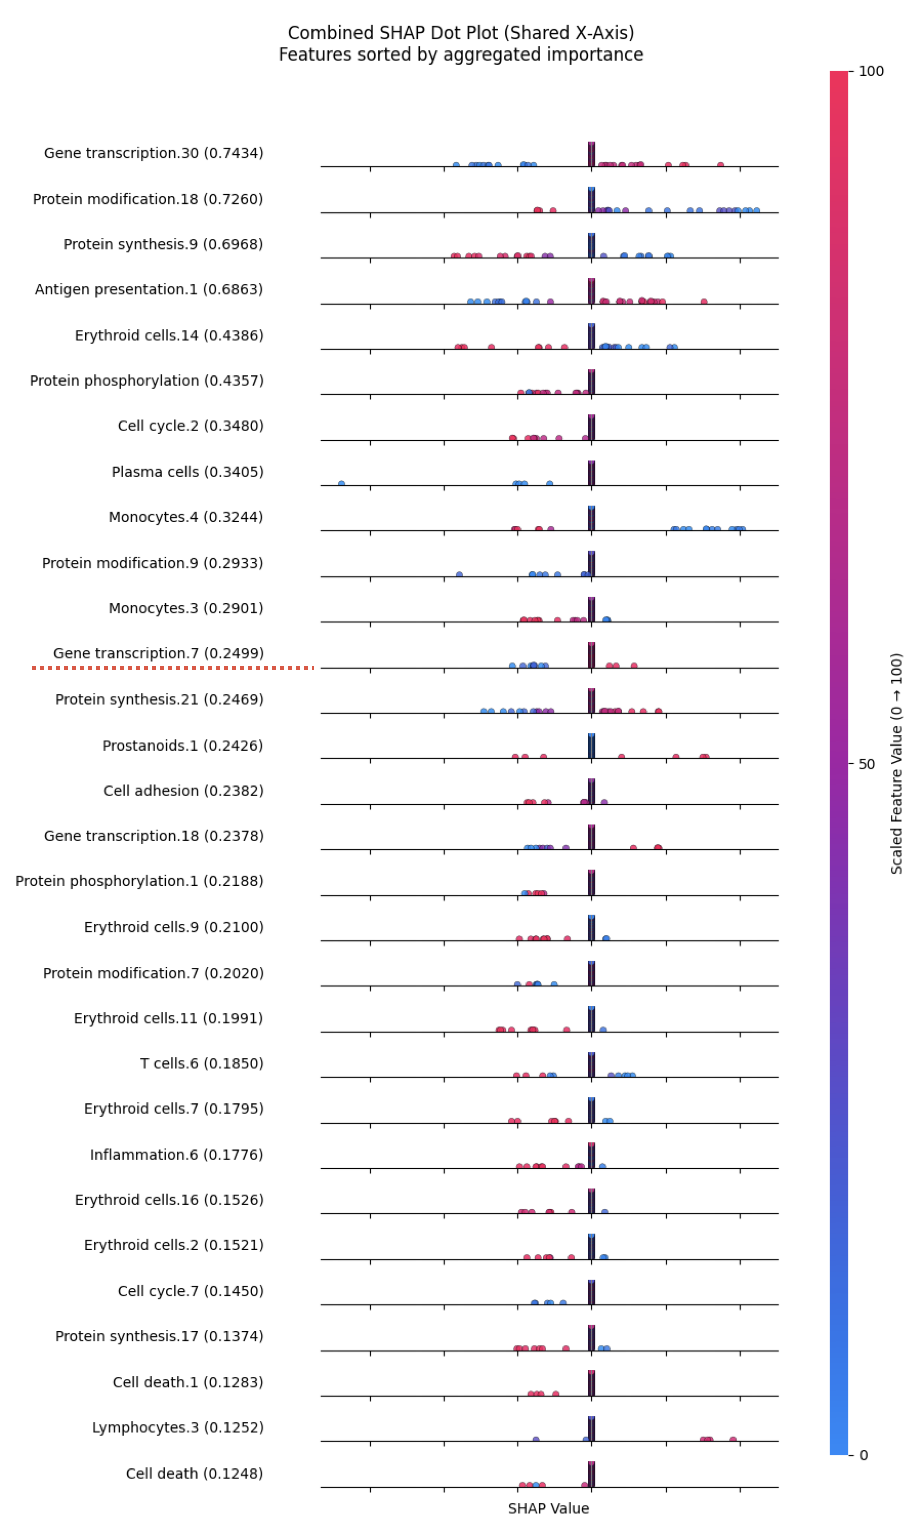
\includegraphics[width=0.85\linewidth]{images/Aggregated_SHAP_RNA_uncompressed.png}
    \caption[Aggregated SHAP plot for SHAP]{Aggregated SHAP summary plot for the SHAP dataset. The same SHAP values are used in the elbow plot shown in Appendix~\ref{appendix:elbow_plots}, Figure~\ref{fig:elbow_plot_rna_uncompressed}, where the cutoff is visualised.}
    \label{fig:rna_aggregated_shap}
\end{figure}

\noindent
Given the large number of features in the \acrshort{rna} dataset (382), the aggregated \gls{shap} summary plot in Figure~\ref{fig:rna_aggregated_shap} displays the top 30 most important features to provide a focused view. To identify the most influential features among these, the "elbow method" was applied to the aggregated \gls{shap} importance values.\\
\\
Based on the elbow point indicated by the dotted line in Figure~\ref{fig:rna_aggregated_shap}, the most influential features for predicting vaccine response are those ranked above this threshold. These top features include: Gene transcription.30 (0.7434), Protein modification.18 (0.7260), Protein synthesis.9 (0.6968), Antigen presentation.1 (0.6863), Erythroid cells.14 (0.4386), Protein phosphorylation (0.4357), Cell cycle.2 (0.3480), Plasma cells (0.3405), Monocytes.4 (0.3244), Protein modification.9 (0.2933), Monocytes.3 (0.2901), and Gene transcription.7 (0.2499).\\
\\
Examining the aggregated \gls{shap} plot for these 12 features reveals consistent patterns in their influence on model output. For features such as Gene transcription.30, Antigen presentation.1, and Gene transcription.7, higher values are associated with positive \gls{shap} values, pushing predictions toward the positive class, while lower values reduce the model's output. In contrast, features like Protein modification.18, Protein synthesis.9, Erythroid cells.14, Monocytes.4 and Monocytes.3 show the opposite pattern: higher values correspond to negative \gls{shap} values, steering predictions toward the negative class, while lower values have a positive effect.

\subsubsection*{Clonal Depth and Breadth Dataset Results}
For the Clonal Depth dataset, the application of the selection criteria resulted in the models listed in Table~\ref{tab:clonal_depth_models} being chosen for aggregated \gls{shap} analysis. These models actually scored very good with a test accuracy of 100\%.\\

\begin{table}[H]
    \centering
    \scalebox{0.85}{
    \begin{tabular}{l l l l l}
        \toprule
        Model & Oversampling & Test Bal. Acc. & Train $p$-val & Train Bal. Acc. ($\mu$/Md) \\
        \midrule
        Random Forest           & smote & 1.0 & 0.029 & 0.696842 \ \ \ / \ \ \ 0.700000 \\
        Logistic Regression     & smote & 1.0 & 0.034 & 0.638033 \ \ \ / \ \ \ 0.641667 \\
        SVM                     & smote & 1.0 & 0.044 & 0.697933 \ \ \ / \ \ \ 0.700000 \\

        Random Forest           & smote-borderline & 1.0 & 0.029 & 0.700858 \ \ \ / \ \ \ 0.700000 \\
        Logistic Regression     & smote-borderline & 1.0 & 0.034 & 0.642033 \ \ \ / \ \ \ 0.641667 \\
        SVM                     & smote-borderline & 1.0 & 0.044 & 0.699200 \ \ \ / \ \ \ 0.704167 \\

        Random Forest           & smote-smotetomek & 1.0 & 0.003 & 0.762267 \ \ \ / \ \ \ 0.766667 \\
        Logistic Regression     & smote-smotetomek & 1.0 & 0.004 & 0.742033 \ \ \ / \ \ \ 0.733333 \\
        SVM                     & smote-smotetomek & 1.0 & 0.000 & 0.770467 \ \ \ / \ \ \ 0.766667 \\
        \bottomrule
    \end{tabular}
    }
    \caption[Selected Models for Clonal Depth]{Models selected for aggregated \gls{shap} analysis for the Clonal Depth dataset.}
    \label{tab:clonal_depth_models}
\end{table}

\begin{figure}[h!]
    \centering
    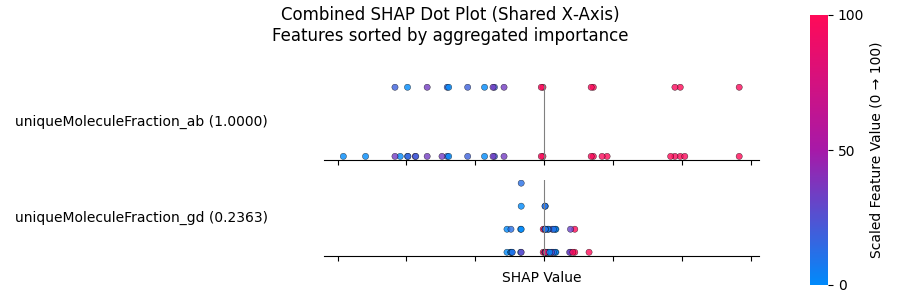
\includegraphics[width=0.85\linewidth]{images/Aggregated_SHAP_Clonal_Depth_selected.png}
    \caption[Aggregated SHAP plot for Clonal Depth]{Aggregated \gls{shap} summary plot for the Clonal Depth dataset.}
    \label{fig:clonal_depth_shap_plot}
\end{figure}
\noindent
Examining the aggregated \gls{shap} plot (Figure~\ref{fig:clonal_depth_shap_plot}) reveals that \texttt{uniqueMoleculeFraction\_ab}, representing the abundance of alpha-beta T cell clones, is by far the most influential feature in the models, with a \gls{shap} importance of 1.0. Higher values of this feature are consistently associated with positive \gls{shap} values. This indicates that individuals with a strong expansion of alpha-beta T cell clones are more likely to have a successful vaccine response. In contrast, \texttt{uniqueMoleculeFraction\_gd}, which captures gamma-delta T cell clonal abundance, has a much lower \gls{shap} importance (0.1580). While it still contributes to the prediction, its influence is significantly less than that of the alpha-beta T cells. This suggests that although gamma-delta T cells may play a supporting role in vaccine response, their clonal expansion is not a primary driver in this dataset.\\
\\
On the other hand, the Clonal Breadth dataset did not yield any models that met the minimum performance criteria. Specifically, no models achieved a test balanced accuracy $\geq 0.5$, a p-value $< 0.05$, and class-specific recall and precision $\geq 0.5$. Despite various modeling attempts, features representing T cell diversity, such as \texttt{fraction\_sequences\_ab} and \texttt{fraction\_sequences\_gd}, did not support reliable model performance. This means the models could not learn any generalizable patterns from these features that would meaningfully distinguish between vaccine responders and non-responders.\\
\\
This suggests that clonal depth (abundance of specific T cell clones) is a more informative and predictive characteristic than clonal breadth (diversity of the T cell repertoire) in this study. While depth appears to reflect a targeted and effective immune response, the broader diversity of T cell sequences alone may not carry enough predictive value for vaccine efficacy in the given context.



\subsection{Addressing Split-Dependency in Small Datasets}
\noindent
While efforts were made to ensure the repeatability of individual experiments by fixing random seeds for all identified sources of randomness (including the initial train-test split, oversampling procedures, and model initialization), it became apparent during the course of this study that the models exhibited a significant degree of split dependency. This was particularly noticeable when altering the random seed used for the initial data split, leading to different model outcomes and performance characteristics across these distinct initializations. This investigation into split dependency was motivated by a need to assess the reliability and stability of the model results and, more specifically, due to the unexpected outcomes observed in the clonal depth and breadth analyses.\\
\\
This challenge is especially pronounced in the context of very small datasets, such as the dataset utilized here. In such scenarios, a single random train-test split, even when consistently reproduced with a fixed seed, can yield training (n=32) and test (n=8) sets that are not truly representative of the overall population distribution. Unlike large datasets where a substantial test set can reliably estimate out-of-sample performance, an n=8 test set is statistically too small to provide a robust or consistently representative "unseen" partition. The specific composition of each split can lead to models learning and prioritizing different patterns, resulting in noticeable shifts in the features deemed important by the model. What is identified as a key predictive feature in one split may lose significance in another, undermining the stability and interpretability of the feature importance results.\\
\\
Furthermore, the interaction between the initial data split and oversampling techniques like \gls{smote} amplifies this issue. Although \gls{smote} is correctly applied only to the training data (n=32), if this small training partition, by chance, contains a biased or unrepresentative subset of the minority class or certain feature combinations, \gls{smote} will generate synthetic samples that reflect and amplify these specific characteristics. Consequently, the models learn patterns that are highly specialized to that particular, augmented training set generated from a specific initial split. When these models are then evaluated on an equally small and potentially distinct n=8 unseen test set (derived from the same initial split), the learned patterns may not generalize well. This explains why changing the initial random seed, which alters both the training and test sets and, subsequently, the synthetic data generated by \gls{smote}, results in different model learning outcomes and performance figures. The models' learned patterns, and thus their stability and perceived performance, become intrinsically tied to the specific composition of the data provided by that particular random split. This is illustrated in Figure~\ref{fig:train_test_split_problem}, where two different train/test splits of the same dataset lead to different regions of synthetic sample generation (shown in blue).

\begin{figure}[h!]
    \centering

    % First row of subfigures (e.g., a & b)
    \begin{subfigure}[b]{0.49\textwidth}
        \centering
        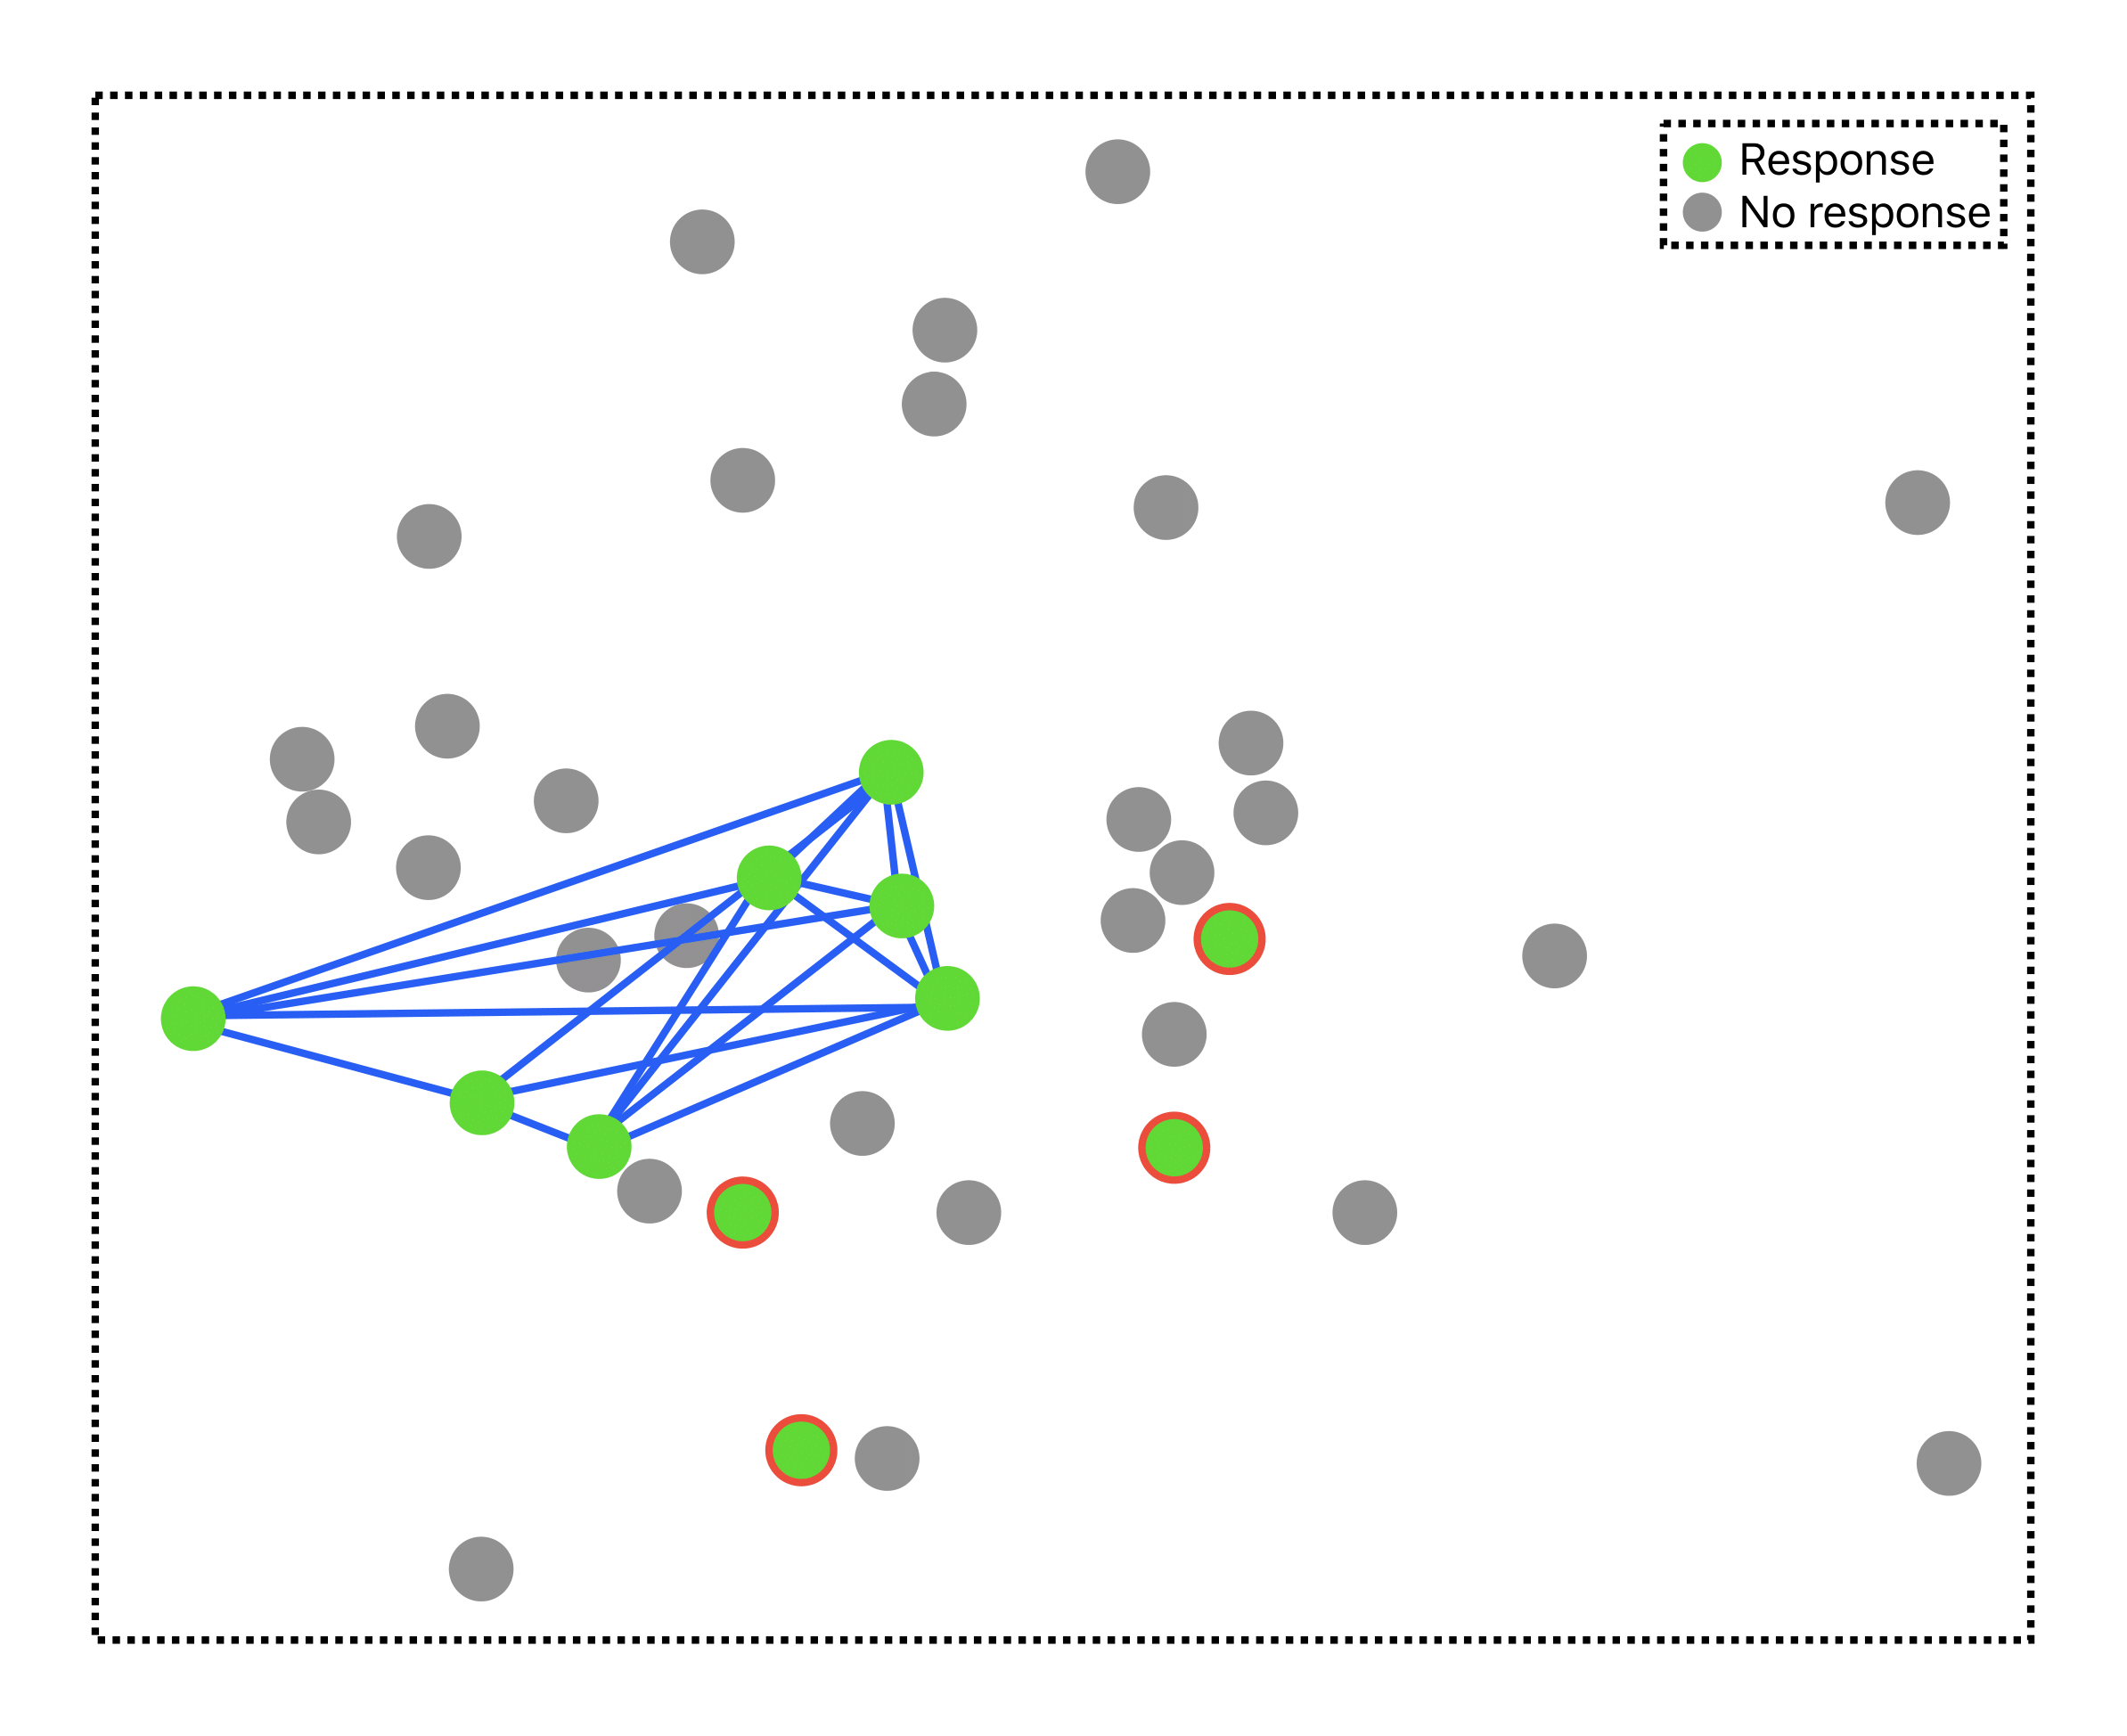
\includegraphics[width=\textwidth]{images/split_problem_1.png}
        \caption{An initial data split of 4 test samples}
        \label{fig:split_problem_1}
    \end{subfigure}
    \hfill
    \begin{subfigure}[b]{0.49\textwidth}
        \centering
        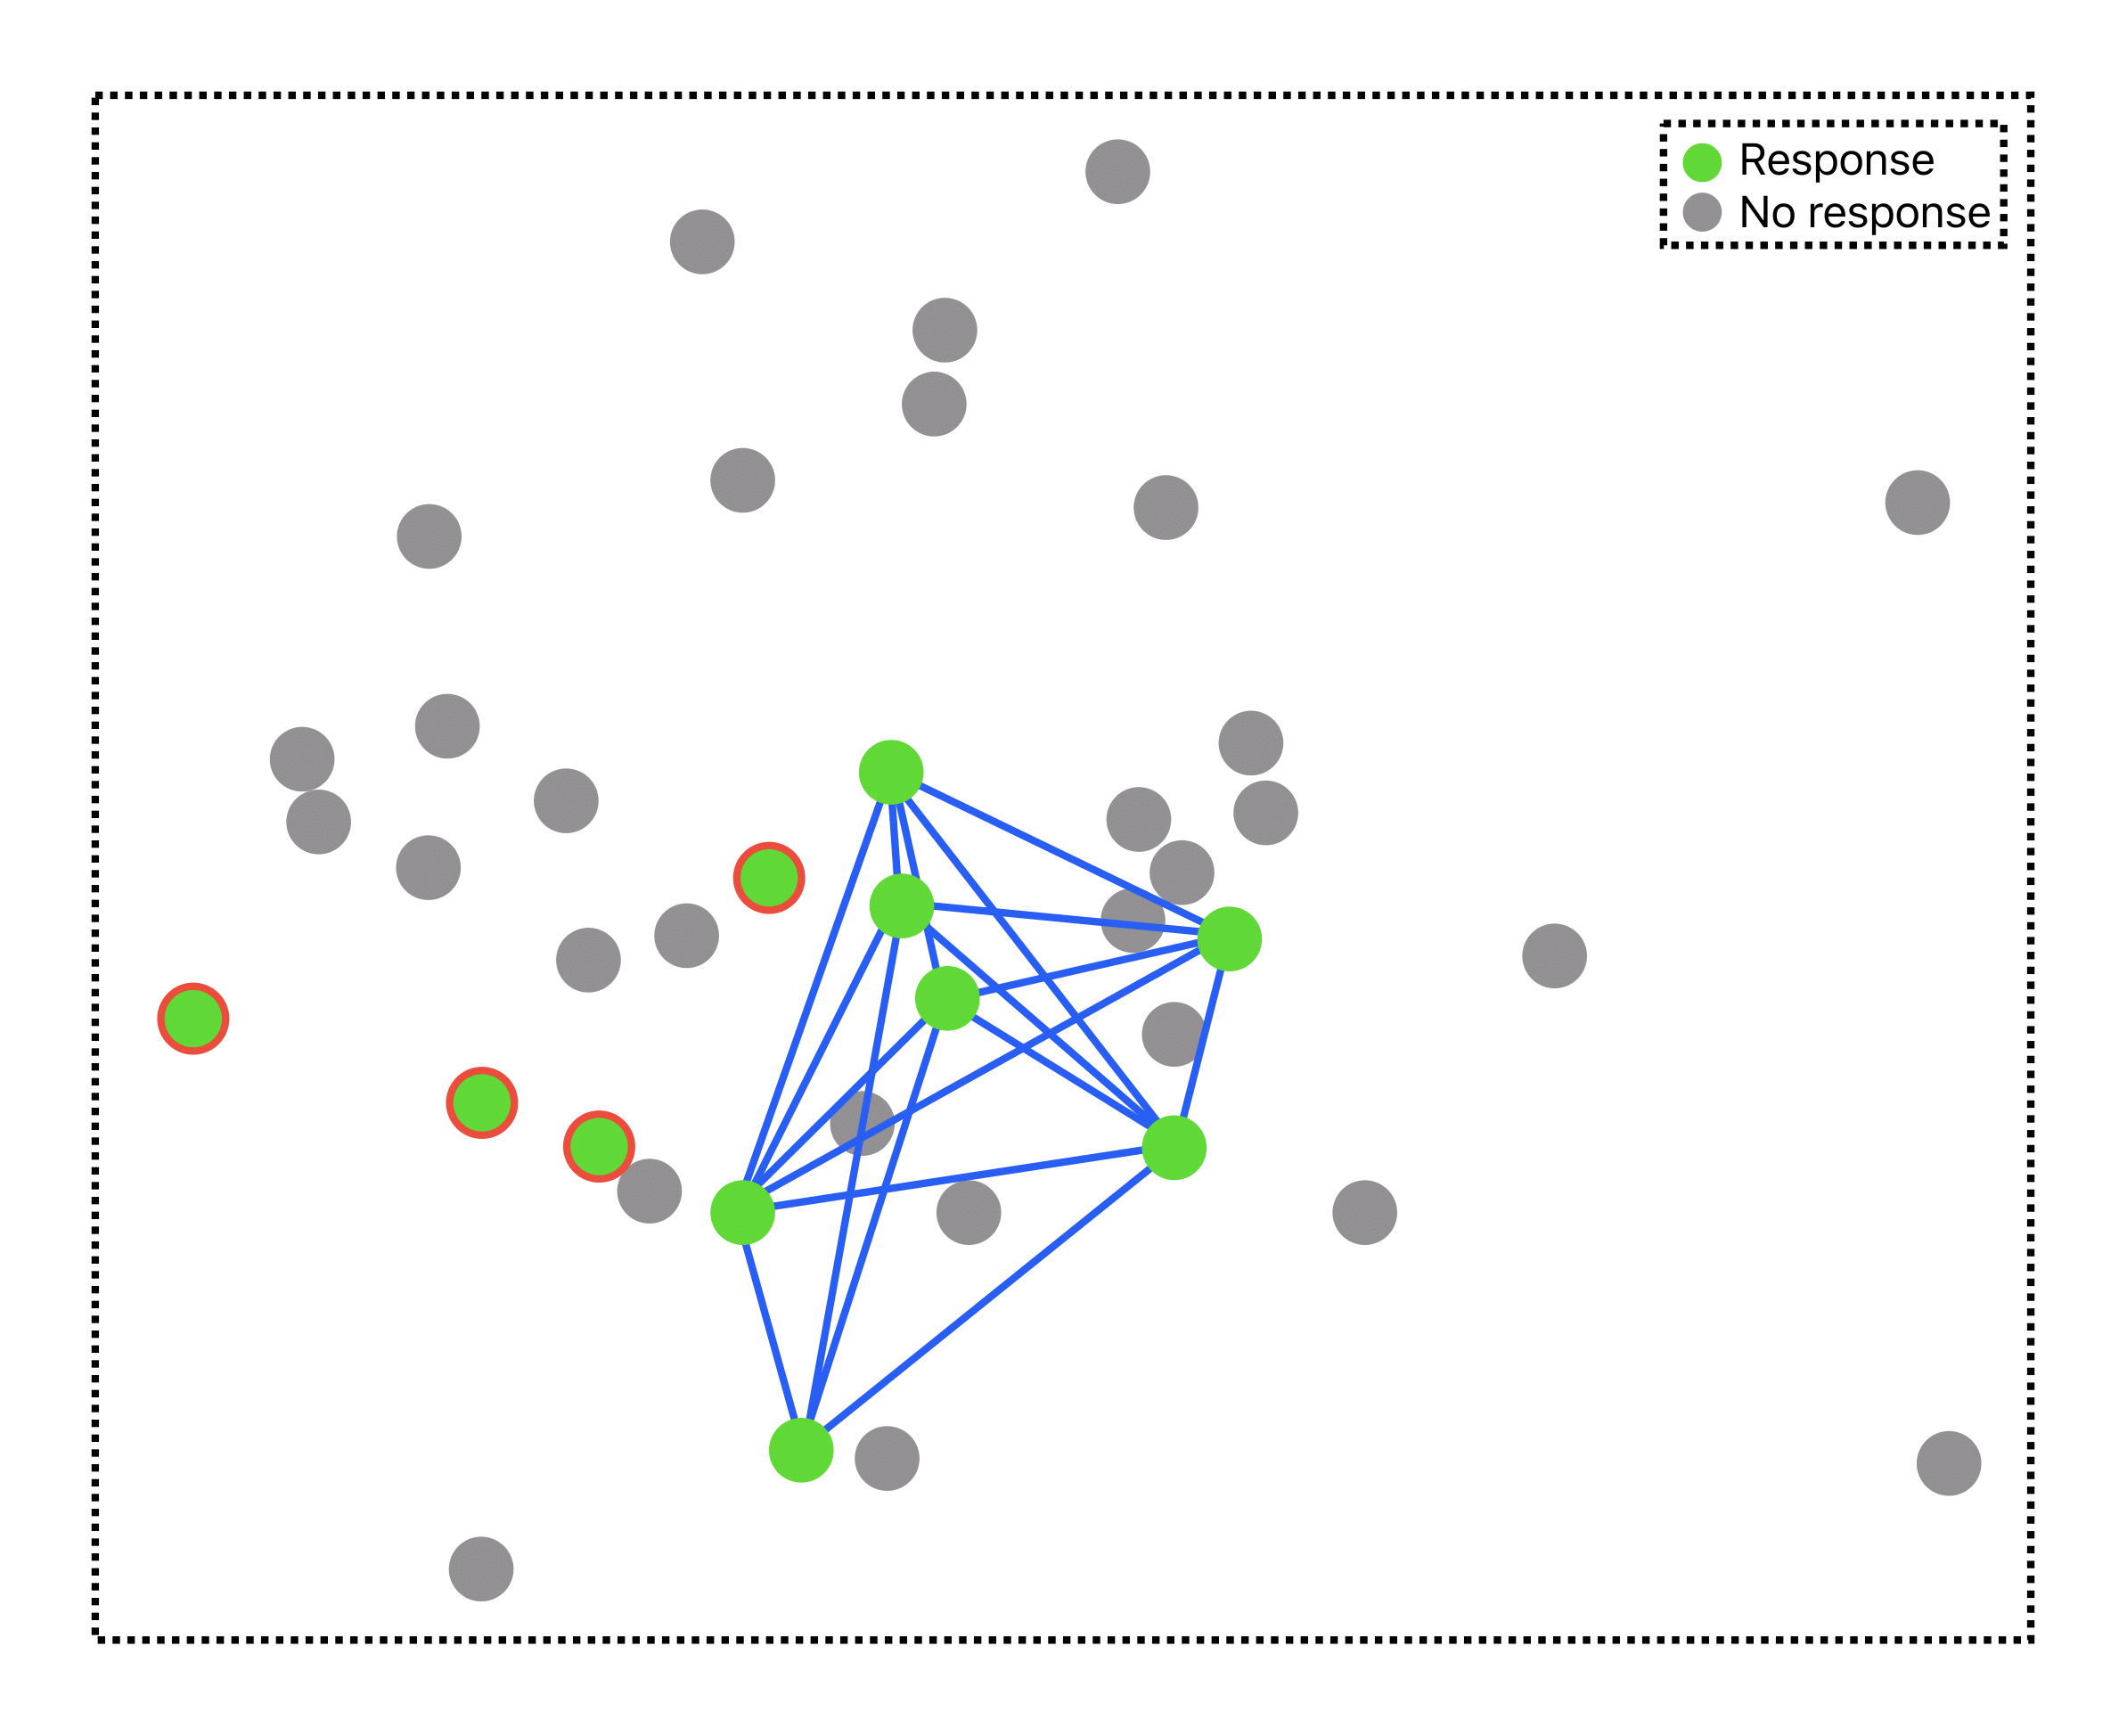
\includegraphics[width=\linewidth]{images/split_problem_2.png}
        \caption{An alternative data split of 4 test samples}
        \label{fig:split_problem_2}
    \end{subfigure}

    \caption[Illustration of Split Dependency]{Illustration of split dependency in small datasets. These two plots show different random train/test splits of the same dataset and demonstrate how the composition of the hold-out test set can vary significantly. This variation directly impacts what the models learn, especially due to the use of \gls{smote} for upsampling. The red samples are the selected test samples for the underrepresented class. The blue regions represent areas where potential synthetic samples can be generated. In (a), the training split leads to \gls{smote} generating samples in one part of the feature space, while in (b), a different split results in synthetic samples being generated in a different region. This means the distribution of the underrepresented class varies substantially between the two splits, leading the models to learn different patterns and ultimately affecting their generalization performance.}
    \label{fig:train_test_split_problem}
\end{figure}

\noindent
To increase the robustness of the analysis, an ideal approach would be to run the full modeling pipeline multiple times and aggregate the results. This would provide a more reliable view of which features are consistently deemed important across different data splits. However, running the complete pipeline once already requires approximately 4~h~35.57~min (16534.37 seconds) of computing time. Due to these time and hardware constraints, it was not feasible to perform repeated runs with full statistical testing. As a compromise, a simplified version of the pipeline was employed. In this version, p-value calculations and bootstrapping were omitted. Instead, a basic k-fold cross-validation was used to estimate the training accuracy. The rest of the pipeline remained the same, with models still being selected for further analysis. However, in place of the statistical p-value threshold, a minimum training accuracy of 0.8 was used as the selection criterion. The other selection metrics remained unchanged. The following subsection evaluates which aspects of the model outcomes generalize across different splits, thereby supporting the relevance of the feature importance results presented in Section~\ref{subsec:feature_identification}.

\subsection{Stability of Model Interpretations Across Splits}
\label{subsec:stability_of_model_interpretations_across_splits}
\noindent
Building upon the recognition of split dependency and its implications for model reliability, an empirical assessment of model interpretation stability was conducted. This analysis aimed to identify features that consistently influence vaccine response across varying data partitions.\\
\\
The approach involved executing the modeling pipeline multiple times, specifically for 100, 200, 300, 400, and 500 iterations. Each iteration employed a different random seed for the initial train-test split. For each dataset and iteration count, the median of the mean absolute SHAP values was computed for all features identified as important by models meeting the predefined selection criteria. This aggregation method served to average out variability and provide a more generalized and robust estimate of feature importance.\\
\\
The analysis of feature importance trajectories across these multiple iterations revealed distinct patterns of convergence (or lack thereof) depending on the dataset characteristics. For instance, in the case of Clonal Depth and Cytometry Data, a clear pattern of convergence was observed (see Figure \ref{fig:trajectory_clonal_depth} and Figure~\ref{fig:trajectory_cytometry}). For clonal depth specifically, the set of identified features after 500 iterations remained very close to those found in the initial single split, reinforcing this stability. These datasets, being inherently lower-dimensional or containing a more focused set of features, allowed feature importance estimates (median of the mean SHAP values) to stabilize relatively quickly. The rank order and magnitudes of important features became consistent as the number of iterations increased. This stability is attributed to the reduced combinatorial complexity and lower risk of correlations inherent in lower-dimensional spaces, which enabled the model's to detect and prioritize meaningful relationships.\\
\\
Conversely, for Clonal Breadth, no strong models were found in the initial split. This may be due to the lack of a clear separation between high feature values and the corresponding outcomes. This supports the earlier finding that Clonal Depth, which reflects the abundance of specific T cell clones, is more informative and predictive than Clonal Breadth. It also shows that alpha-beta T cells are consistently better predictors than gamma-delta T cells in this study.\\
\\
Regarding the Cytokines dataset, while the precise feature importance values from the initial split were not entirely consistent with those observed after 500 iterations, the directional patterns of these features remained robust. That is, when a high feature value shifted the prediction toward a specific class, this influence remained consistent across different splits. This pattern is similar to the stability seen with clonal depth, even if the exact importance scores changed.

\begin{figure}[H]
    \centering
    \begin{subfigure}[b]{0.48\textwidth}
        \centering
        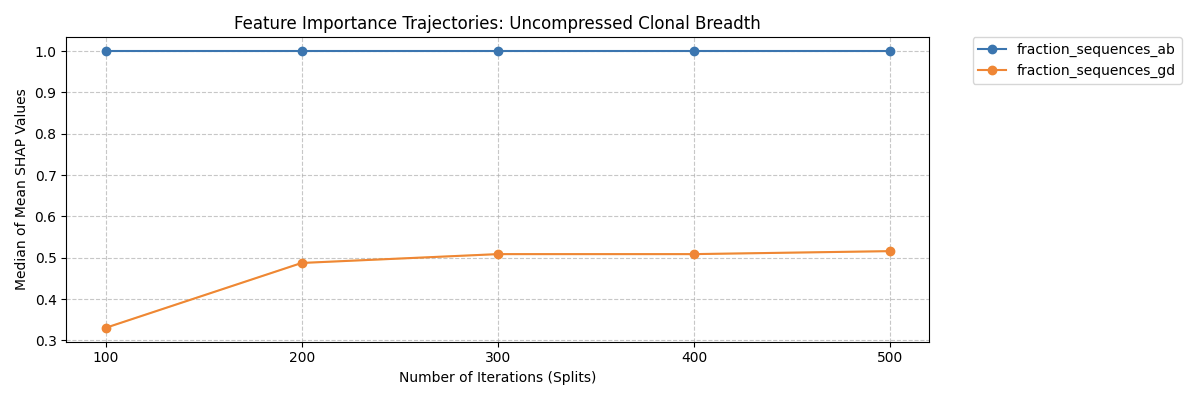
\includegraphics[width=\textwidth]{images/trajectory_clonal_breadth.png}
        \caption{trajectory clonal breadth}
        \label{fig:trajectory_clonal_breadth}
    \end{subfigure}
    \hfill
    \begin{subfigure}[b]{0.48\textwidth}
        \centering
        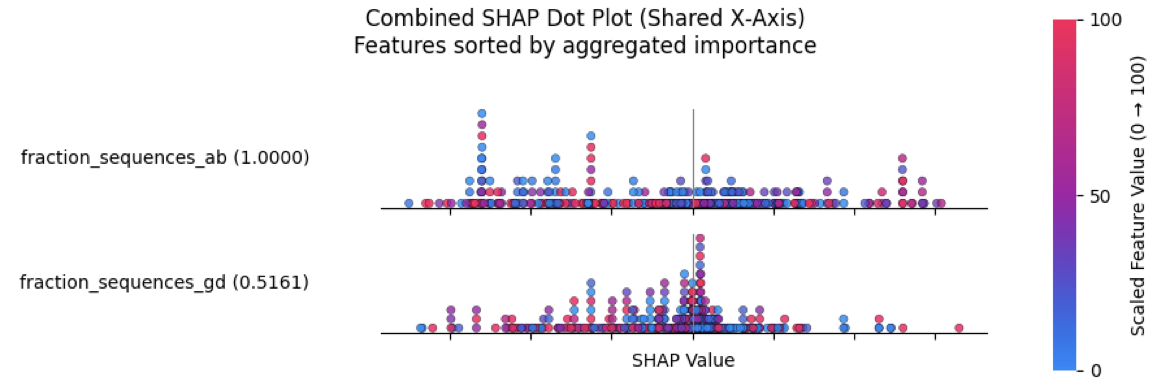
\includegraphics[width=\textwidth]{images/stable_features_clonal_breadth.png}
        \caption{Stable Features clonal breadth}
        \label{fig:stable_features_clonal_breadth}
    \end{subfigure}

    \begin{subfigure}[b]{0.48\textwidth}
        \centering
        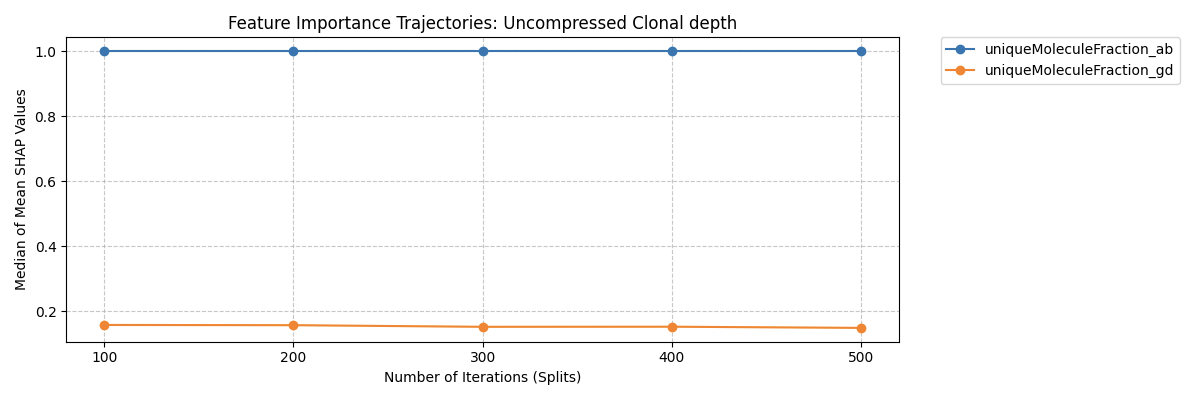
\includegraphics[width=\textwidth]{images/trajectory_clonal_depth.png}
        \caption{trajectory clonal depth}
        \label{fig:trajectory_clonal_depth}
    \end{subfigure}
    \hfill
    \begin{subfigure}[b]{0.48\textwidth}
        \centering
        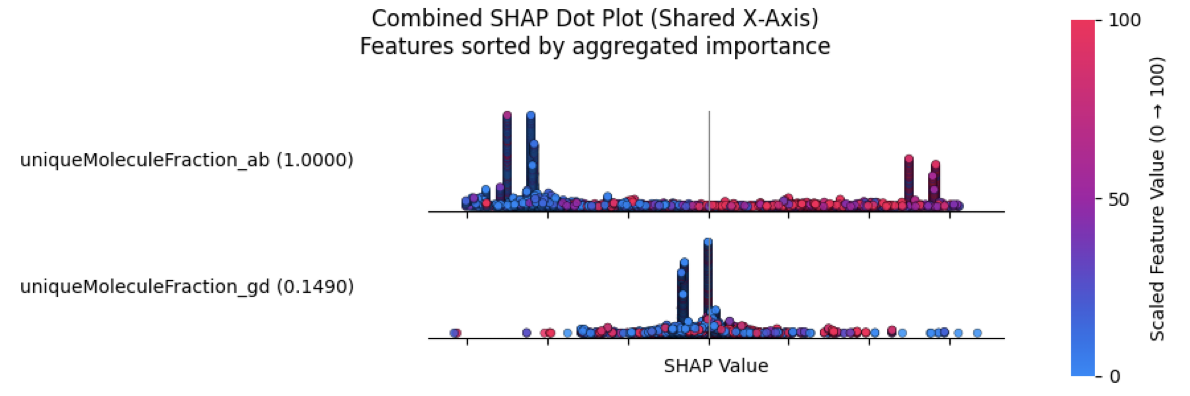
\includegraphics[width=\textwidth]{images/stable_features_clonal_depth.png}
        \caption{Stable Features clonal depth}
        \label{fig:stable_features_clonal_depth}
    \end{subfigure}

    \begin{subfigure}[b]{0.48\textwidth}
        \centering
        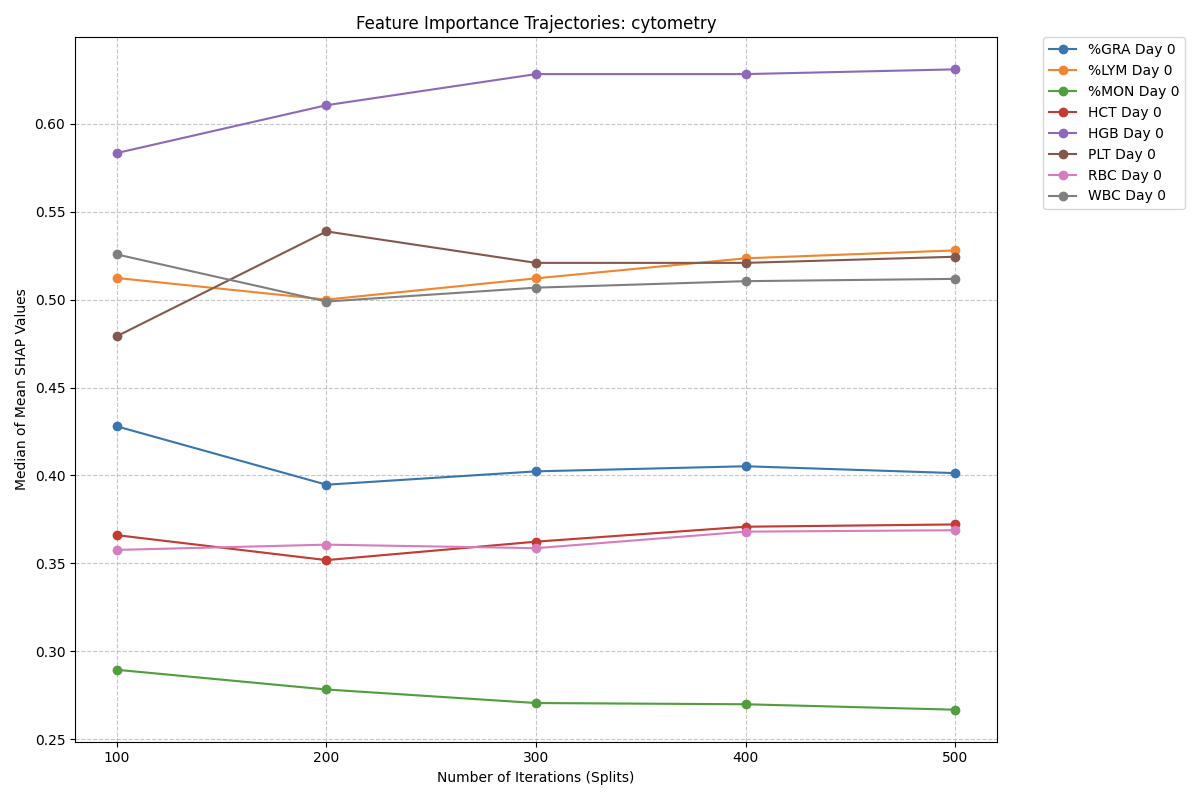
\includegraphics[width=\textwidth]{images/trajectory_cytometry.png}
        \caption{trajectory cytometry}
        \label{fig:trajectory_cytometry}
    \end{subfigure}
    \hfill
    \begin{subfigure}[b]{0.48\textwidth}
        \centering
        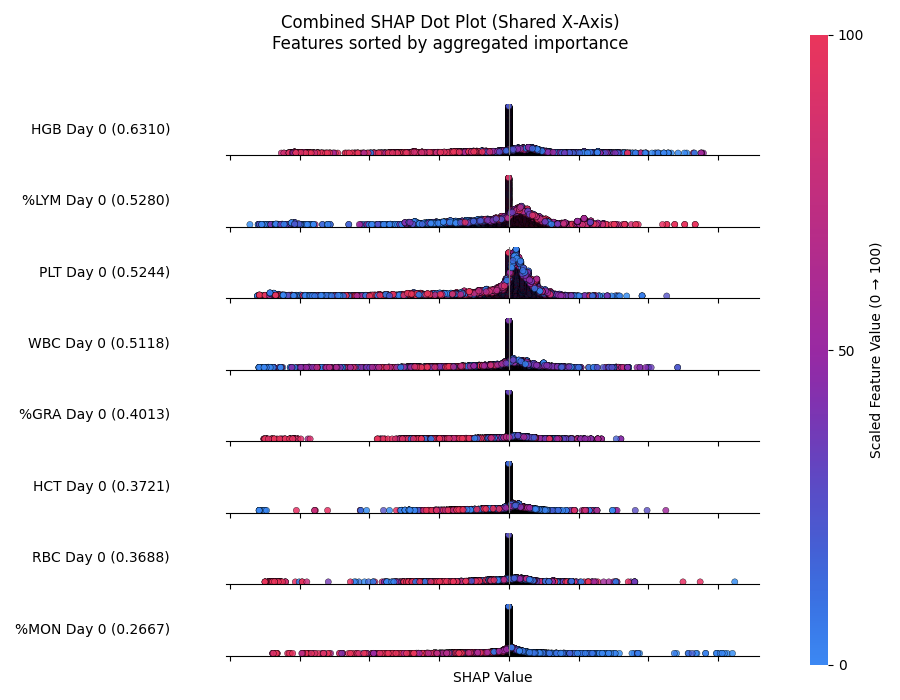
\includegraphics[width=\textwidth]{images/stable_features_cytometry.png}
        \caption{Stable Features cytometry}
        \label{fig:stable_features_cytometry}
    \end{subfigure}

    \caption[Feature Importance Trajectories and Stable Features 1]{Visual representation of feature importance convergence. The left column shows the trajectory of feature importance across 100, 200, 300, 400, and 500 iterations for converging datasets (e.g., Clonal Breadth, Clonal Depth, or Cytometry). The right column displays the stable feature importance after 500 iterations.}
    \label{fig:feature_trajectories_plots}
\end{figure}

\noindent
Despite having only 40 features, the Cytokines dataset exhibited persistent instability and a notable lack of clear convergence (see Figure \ref{fig:trajectory_cytokienes}). This is illustrated by features like TNFa, which was deemed important enough to be included in the top list after 100 splits but completely dropped out (or its importance fell below the display threshold) when aggregated over 500 iterations. Such disappearing features strongly indicate an unreliable perceived importance. Furthermore, other features showed substantial shifts in their attributed importance across iterations; for instance, HHV6.Status fluctuated significantly (e.g., from 0.2434 at 100 splits to 0.2085 at 500 splits, with intermediate values like 0.2834), as did IL-7 (from 0.0355 at 100 splits to 0.1126 at 500 splits) and IL-9 (starting at 0 at 100 splits and reaching 0.1287 at 500 splits, notably appearing only after 300 splits). This persistent instability suggests that, even with a moderate number of features, the high-dimensional space relative to the small sample size (N=40) and potential correlations allows models to pick different, equally valid, subsets of features across various random splits, leading to highly fluctuating individual feature importance. This implies the dataset likely contains a considerable amount of noise or lacks a strong, consistent signal for the predictive task.\\
\\

\begin{figure}[h!]
    \centering
    \begin{subfigure}[b]{0.48\textwidth}
        \centering
        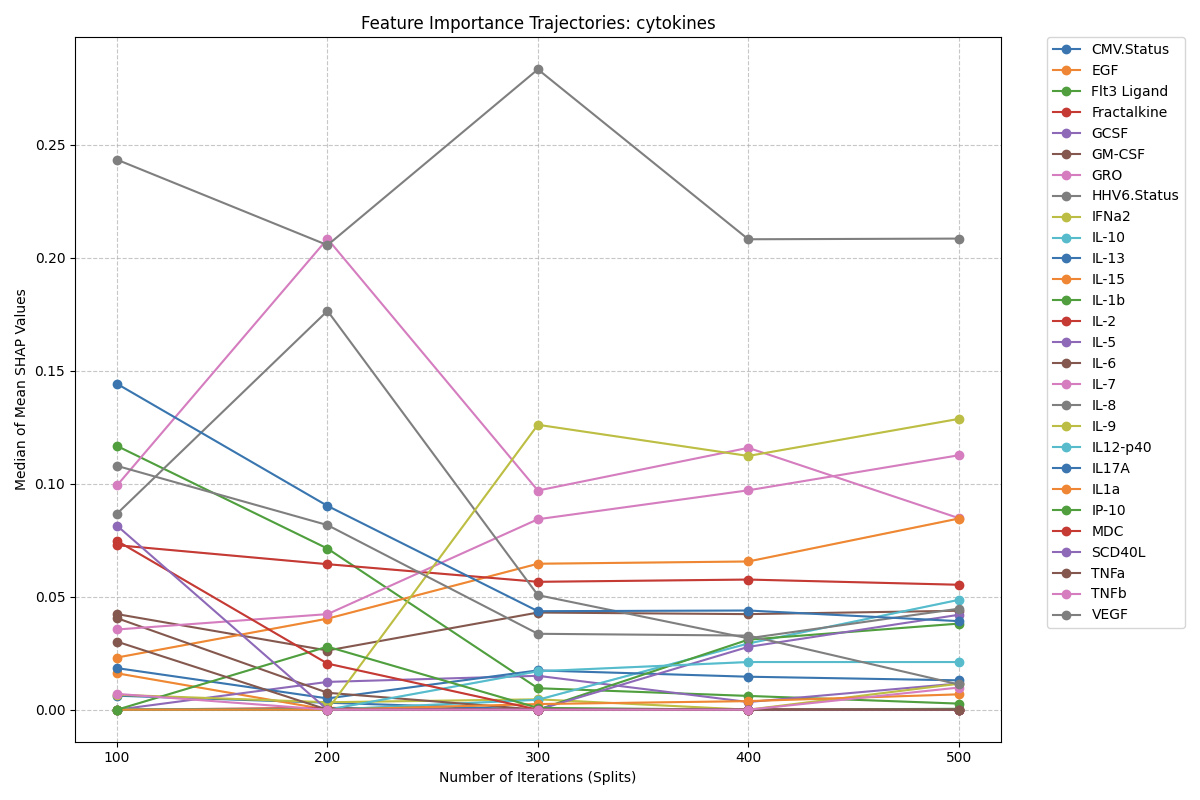
\includegraphics[width=\textwidth]{images/trajectory_cytokienes.png}
        \caption{trajectory cytokines}
        \label{fig:trajectory_cytokienes}
    \end{subfigure}
    \hfill
    \begin{subfigure}[b]{0.48\textwidth}
        \centering
        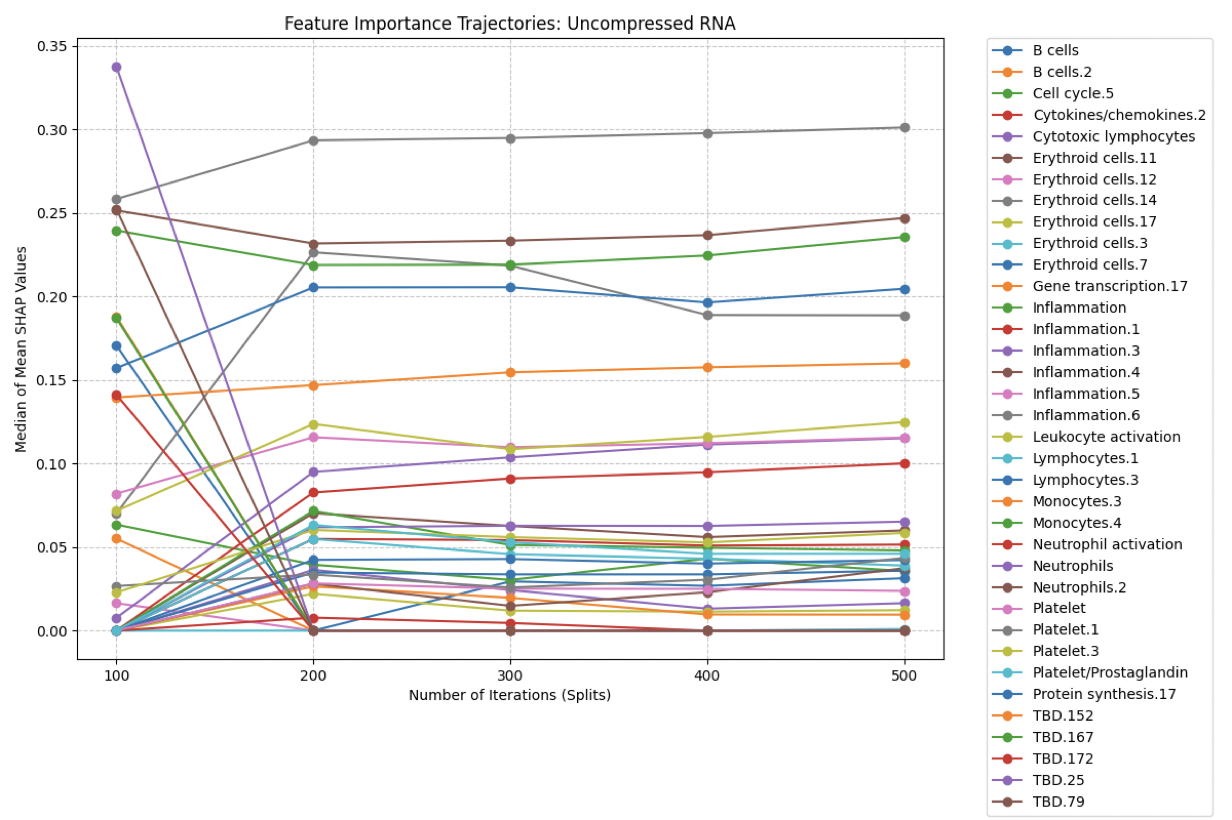
\includegraphics[width=\textwidth]{images/trajectory_RNA.png}
        \caption{trajectory \acrshort{rna}}
        \label{fig:trajectory_RNA}
    \end{subfigure}

    \begin{subfigure}[b]{0.48\textwidth}
        \centering
        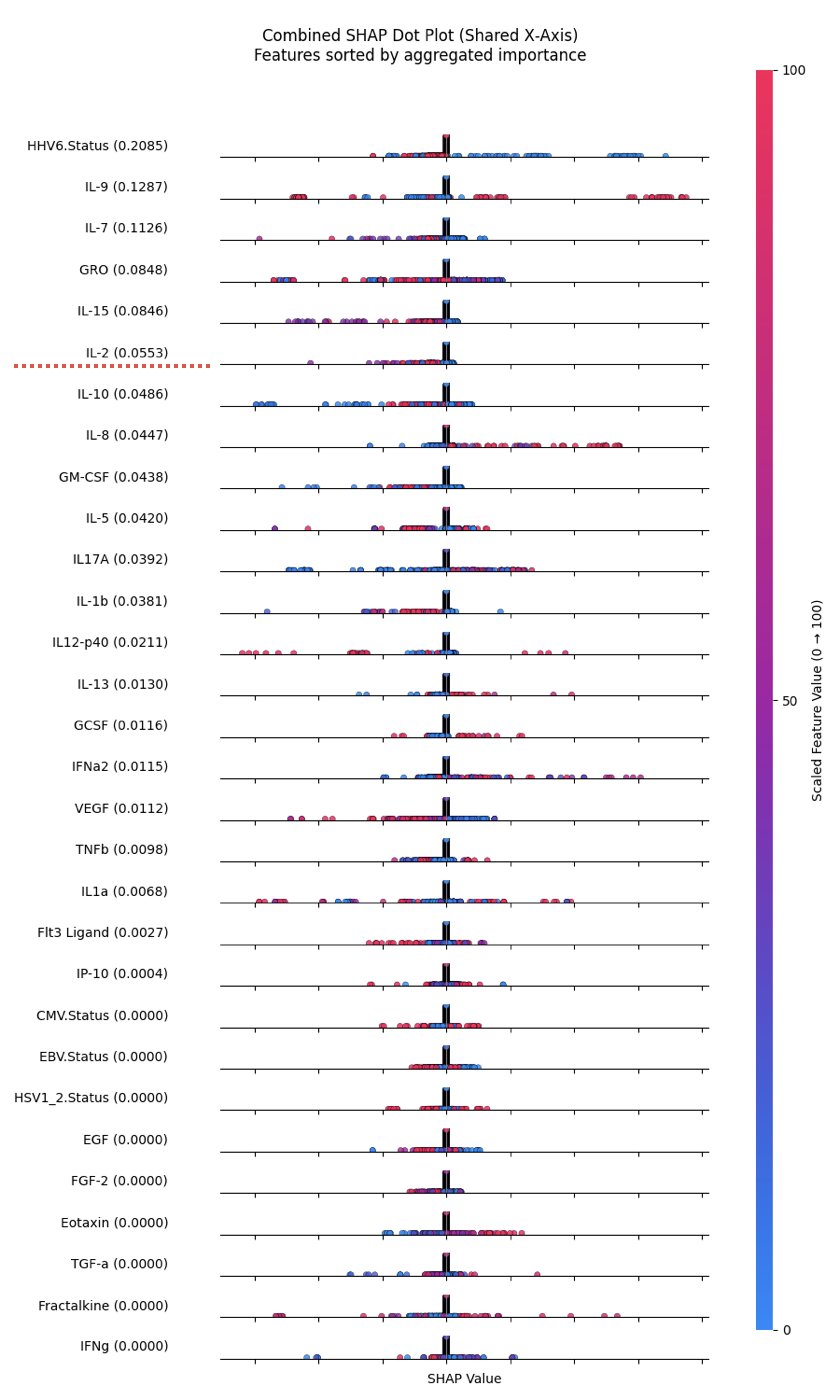
\includegraphics[width=\textwidth]{images/stable_features_cytokines.png}
        \caption{Stable Features cytokines}
        \label{fig:stable_features_cytokines}
    \end{subfigure}
    \hfill
    \begin{subfigure}[b]{0.48\textwidth}
        \centering
        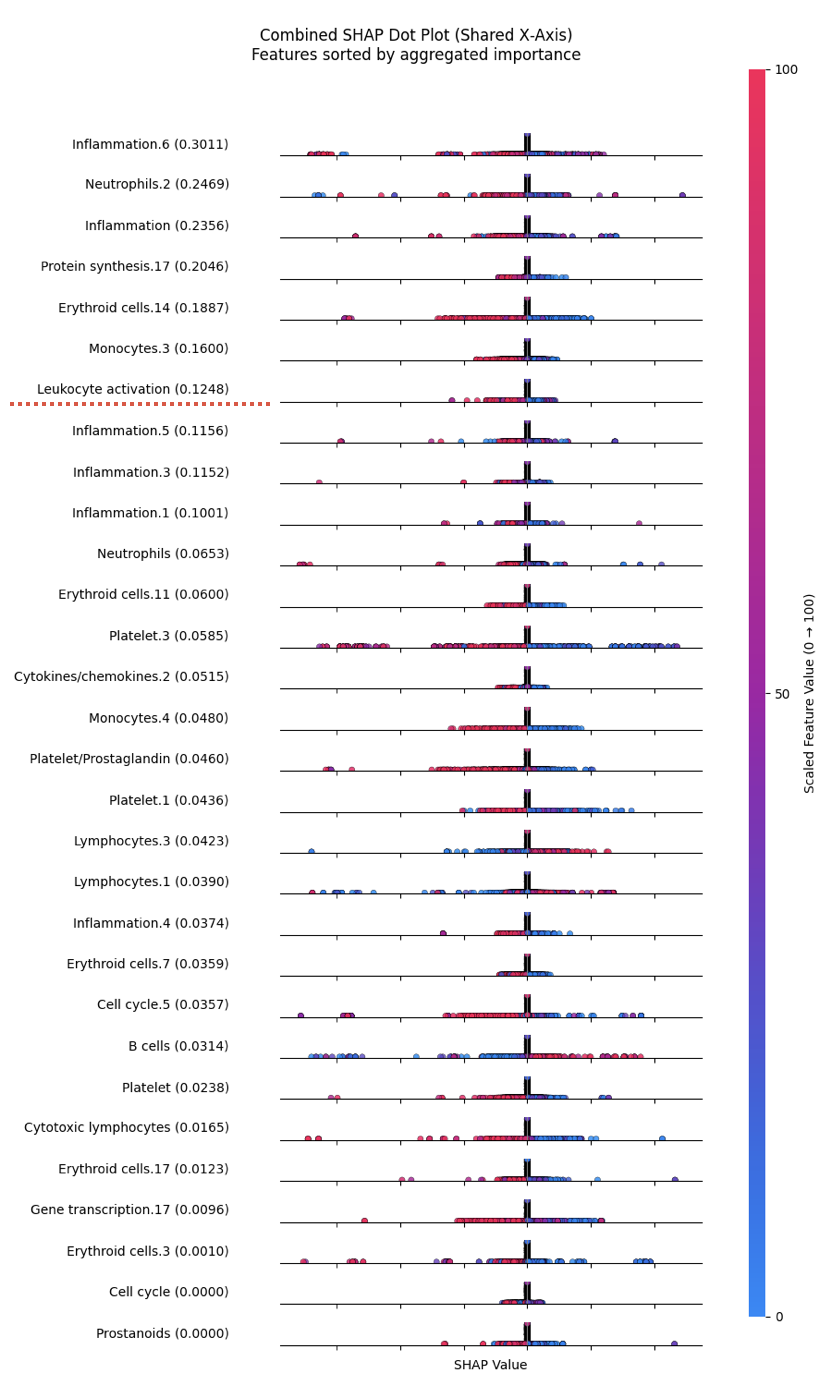
\includegraphics[width=\textwidth]{images/stable_features_RNA.png}
        \caption{Stable Features \acrshort{rna}}
        \label{fig:stable_features_RNA}
    \end{subfigure}

    \caption[Feature Importance Trajectories and Stable Features 2]{Visual representation of feature importance convergence. The top row shows the trajectory of feature importance across 100, 200, 300, 400, and 500 iterations for converging datasets (e.g., cytokines and \acrshort{rna} data). The bottom row displays the 'stable' feature importance after 500 iterations.}
    \label{fig:feature_trajectories_plots2}
\end{figure}
\noindent
The \acrshort{rna} dataset, with its significantly higher dimensionality (382 features), also showed signs of instability, akin to the Cytokines data. For instance, features like TBD.25 and TBD.79, which were present in the 100-split aggregated results, were not present by 500 splits, indicating a shift in the identified top features (see Figure \ref{fig:trajectory_RNA}). However, when compared to the Cytokines data, the \acrshort{rna} data showed some indications of converging, suggesting that despite its higher dimensionality, a discernible signal might still be present.\\
\\
Recognizing the persistent instability observed in the high-dimensional datasets, particularly Cytokines and \acrshort{rna}, and building upon the identification of correlating features as detailed in Section~\ref{sec:correlation_analysis_within_individual_datasets}, the role of feature compression was further investigated. The underlying hypothesis was that actively reducing noise and redundancy inherent in these correlated feature sets through compression would lead to more stable and reliable feature importance estimates. While our approach focused on clustering-based compression, it is important to note that other techniques for dimensionality reduction, such as Lasso regularization, which can intrinsically drive the importance of certain features to zero, could also serve as valuable alternative strategies to enhance model interpretability and stability.\\
\\
For the compressed \acrshort{rna} data, a noticeable improvement in stability was observed. The largest absolute changes in median \gls{shap} values between 100 and 500 iterations were generally smaller (around $\approx$0.06 to $\approx$0.07) compared to the uncompressed \acrshort{rna} data. Crucially, the set of identified compressed features (clusters) remained largely consistent across 100 and 500 iterations, indicating that compression helped to identify a more robust and consistently important set of underlying patterns (Figure~\ref{fig:trajectory_RNA_compressed}).\\
\\
The compressed Cytokines data also demonstrated an improvement in stability compared to its uncompressed counterpart, although it still did not fully converge to a perfectly stable state across all features. For instance, the median mean \gls{shap} value for GRO\_Compressed exhibited fluctuations (e.g., from 0.8564 at 100 iterations, peaking at 1.0 at 400 iterations, and settling at 0.8340 at 500 iterations). Similarly, HHV6.Status, though a less prominent feature, showed considerable variability (from 0.4319 at 100 iterations, dropping to 0 by 300 iterations, and then reappearing at 0.1103 at 500 iterations in its compressed form) as can be seen in Figure~\ref{fig:trajectory_cytokienes_compressed}. This behavior, where magnitudes adjust significantly (either increasing, decreasing, or even temporarily disappearing and reappearing), is interpreted as the model's iterative process converging towards a more confident and realistic estimate of the feature's true importance as noise from individual splits is progressively averaged out. A key distinction from the uncompressed data is that, even with these fluctuations, the set of important compressed features tended to remain consistent, with fewer features entirely dropping out from the top list.\\
\\
Some features show a median mean \gls{shap} value of 0, both in compressed and uncompressed sets (see Figures~\ref{fig:stable_features_cytokines} and \ref{fig:stable_features_cytokines_compressed}). This means they had no consistent influence on the model. Their effect was either weak, inconsistent, or canceled out across splits. This suggests they lack predictive power or behave like noise. In the uncompressed Cytokines data, this pattern was already visible. Even with fewer features, instability persisted. This points to a weak or noisy signal. When features still score 0 after many iterations, it confirms they contribute little or nothing to the prediction.\\
\\
\begin{figure}[H]
    \centering
    \begin{subfigure}[b]{0.48\textwidth}
        \centering
        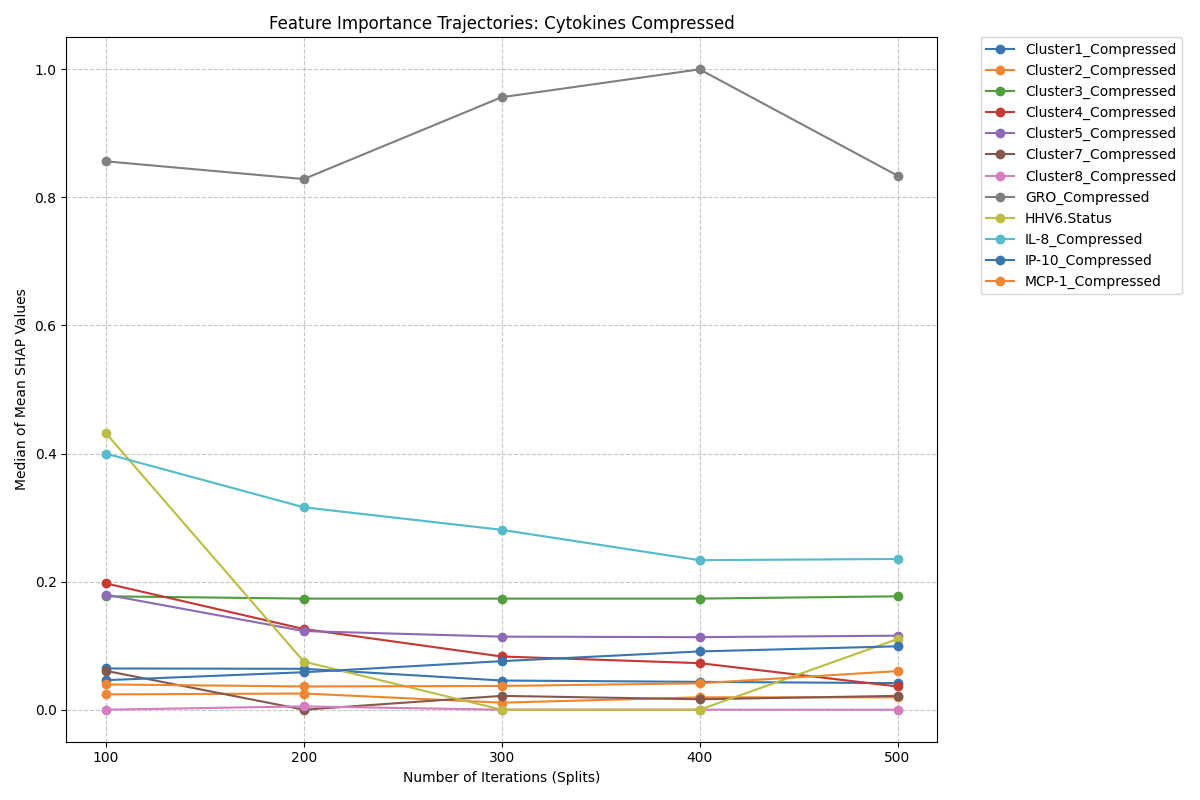
\includegraphics[width=\textwidth]{images/trajectory_cytokienes_compressed.png}
        \caption{trajectory cytokines compressed}
        \label{fig:trajectory_cytokienes_compressed}
    \end{subfigure}
    \hfill
    \begin{subfigure}[b]{0.48\textwidth}
        \centering
        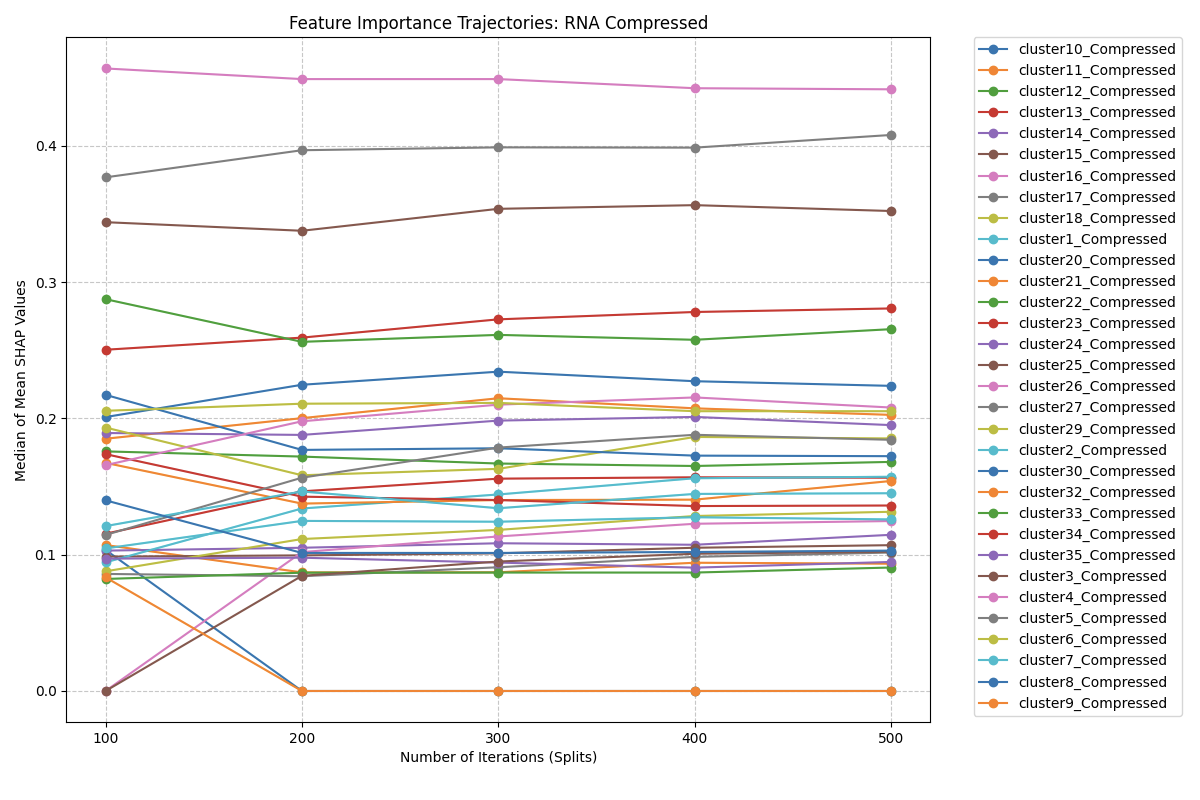
\includegraphics[width=\textwidth]{images/trajectory_RNA_compressed.png}
        \caption{trajectory \acrshort{rna} compressed}
        \label{fig:trajectory_RNA_compressed}
    \end{subfigure}

    \begin{subfigure}[b]{0.48\textwidth}
        \centering
        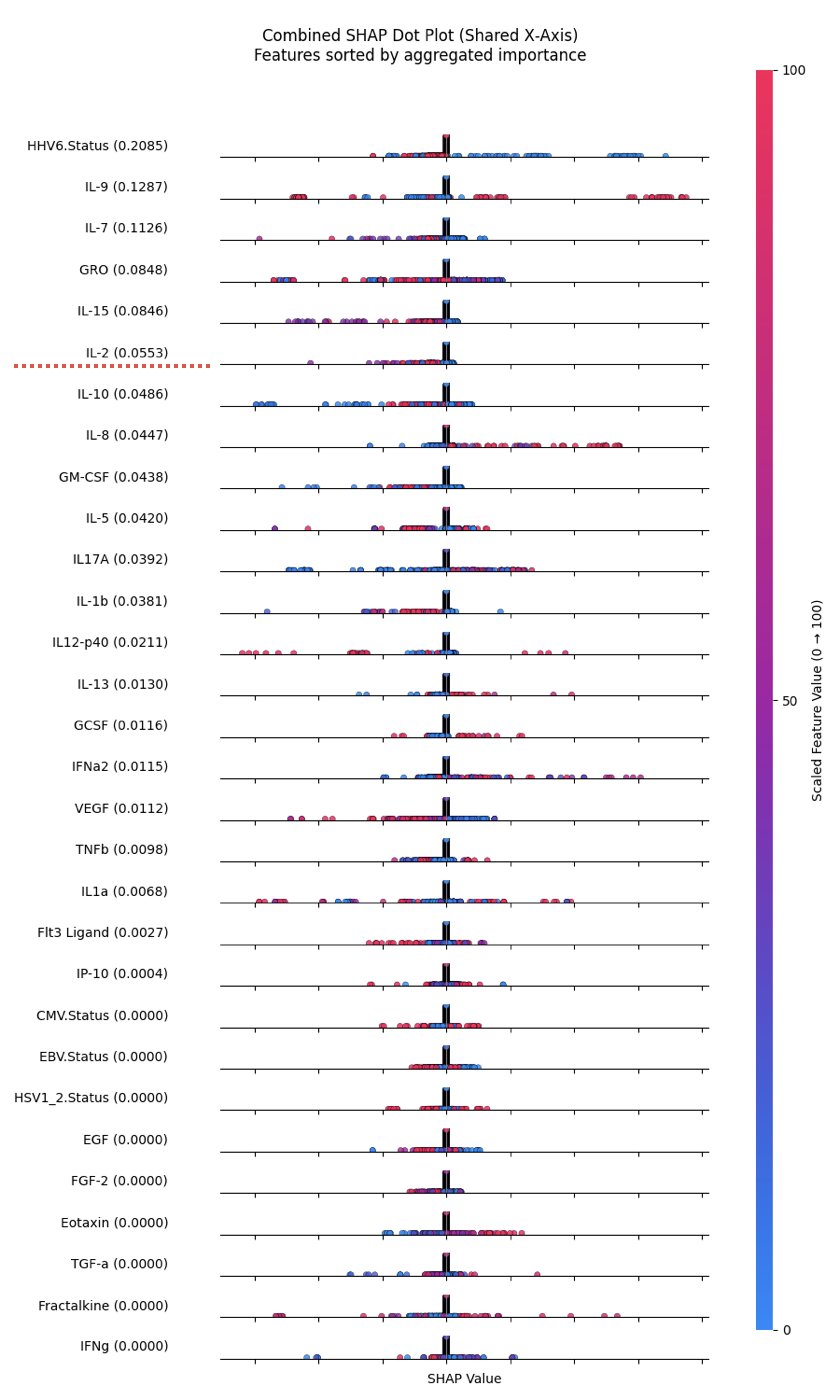
\includegraphics[width=\textwidth]{images/stable_features_cytokines.png}
        \caption{Stable Features cytokines compressed}
        \label{fig:stable_features_cytokines_compressed}
    \end{subfigure}
    \hfill
    \begin{subfigure}[b]{0.48\textwidth}
        \centering
        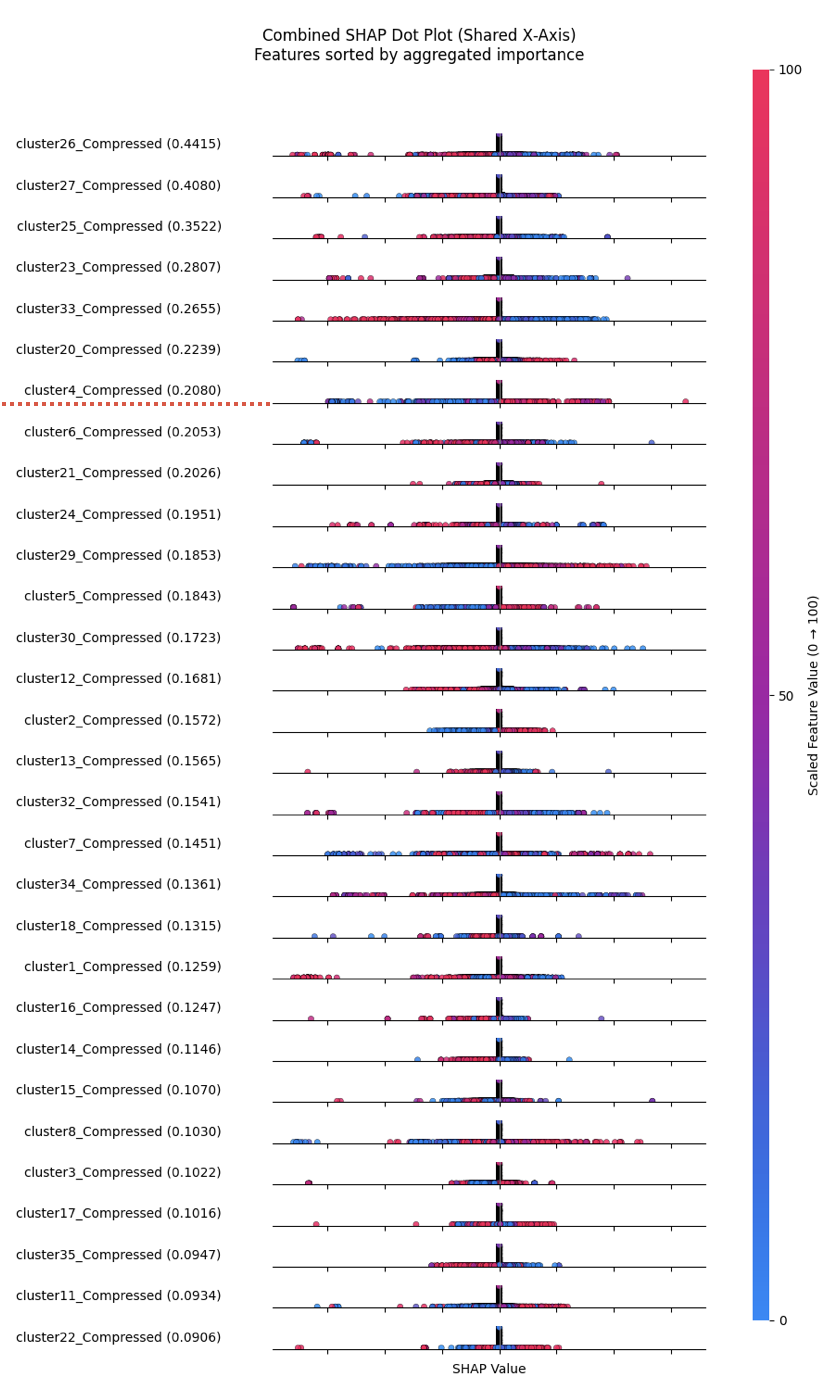
\includegraphics[width=\textwidth]{images/stable_features_RNA_compressed.png}
        \caption{Stable Features \acrshort{rna} compressed}
        \label{fig:stable_features_RNA_compressed}
    \end{subfigure}

    \caption[Feature Importance Trajectories and Stable compressed Features]{Visual representation of feature importance convergence. The top row shows the trajectory of the compressed feature importance across 100, 200, 300, 400, and 500 iterations for converging datasets (e.g., cytokines and \acrshort{rna} data). The bottom row displays the stable compressed feature importance after 500 iterations.}
    \label{fig:feature_trajectories_plots3}
\end{figure}
\pagebreak
\noindent
The empirical assessment of feature importance stability across numerous iterations and data partitions leads to several critical conclusions regarding the reliability of our model interpretations.\\
\\
Firstly, a highly robust finding across all datasets is the consistent directional influence of features. Regardless of compression applied or fluctuations in their absolute importance ranking, if a feature's higher values consistently pushed predictions towards a specific class in one split, this qualitative relationship was preserved across all iterations. This consistent directional impact provides a reliable and biologically interpretable basis for understanding feature effects, even when quantitative importance scores vary.\\
\\
Secondly, datasets that are inherently lower-dimensional, such as Clonal Depth and Cytometry data, consistently exhibit greater stability in feature importance. This confirms that a simpler feature space is less prone to the ambiguities and random variations that inherently challenge model learning in high-dimensional, low-sample-size settings. For these datasets, the observed convergence of \gls{shap} values provides confidence in the identified key features.\\
\\
Thirdly, for high-dimensional datasets like \acrshort{rna} and Cytokines, compressing features proved to be an effective and often necessary strategy for achieving more stable and reliable feature importance estimates within practical computational constraints. The primary benefit of compression lies in the increased consistency of which features (or feature clusters) are identified as important across different data views, significantly reducing the issue of features appearing and disappearing from the top ranks due to random sampling variations.\\
\\
Finally, the persistent instability observed in the uncompressed Cytokines data, even after 500 iterations, coupled with the fact that even compressed Cytokines data still required significant adjustments to converge, strongly suggests that this dataset may not carry a sufficiently strong or clear predictive signal for the given response labels. While compression successfully distills and clarifies the available signal, it cannot inherently create a strong signal where none exists. This implies the Cytokines dataset is likely inherently "noisy" or less informative for the specific predictive task. This explains why some features consistently registered zero importance, as they provide negligible or inconsistent contributions to the model's predictions.

\section{Code Availability}
\noindent
All code and scripts used for data processing, model training, and analysis are publicly available on GitHub at https://github.com/Elias-Dams/multimodal-data-integration-predictive-modeling-measles-vaccine-response-cross-validation.

%%%%%%%%%%%%%%%%%%%%%%%%%%%%%%%%%%%%%%%%%%%%%%%%%%%%%%%%%%%%%%%%%%%%%%%%%%%%%%%%%%%%%%%%%%%%%%%%%%%%%%%%%%%%%%%%%%%%%%%%%%%%%%%%%%%%%%%%%%%%%%%%%









\chapter{Cross-Vaccine Marker Validation with Hepatitis B}
%%%%%%%%%%%%%%%%%%%%%%%%%%%%%%%%%%%%%%%%%%%%%%%%%%%%%%%%%%%%%%%%%%%%%%%%%%%%%%%%%%%%%%%%%%%%%%%%%%%%%%%%%%%%%%%%%%%%%%%%%%%%%%%%%%%%%%%%%%%%%%%%%
% \todo{Describe the application of the same pipeline to the hepatitis B dataset, compare predictive features, and discuss the validation process.}
%%%%%%%%%%%%%%%%%%%%%%%%%%%%%%%%%%%%%%%%%%%%%%%%%%%%%%%%%%%%%%%%%%%%%%%%%%%%%%%%%%%%%%%%%%%%%%%%%%%%%%%%%%%%%%%%%%%%%%%%%%%%%%%%%%%%%%%%%%%%%%%%%


\noindent
This chapter details the attempt to validate the generalizability of predictive markers and models identified in the measles vaccine response study by applying them to an independent hepatitis B dataset.

\section{Validation Cohort Setup and Comparative Labeling}
\noindent
To confirm the generalizability of findings derived from the measles study it was essential to validate the approach on an independent cohort. For this purpose, the hepatitis B dataset was utilized as a distinct validation cohort.\\

\begin{figure}[h!] 
    \centering 

    % First row of subfigures (e.g., a & b)
    \begin{subfigure}[b]{0.49\textwidth}
        \centering
        \includegraphics[width=\textwidth]{images/Antibody_Titer_Trajectories_for_Hepatitis_original.png} 
        \caption{Original Pre-Determined Converter Status (Early, Late, and Non-Converters)} 
        \label{fig:antibody_titer_hepatitis_original}
    \end{subfigure}
    \hfill
    \begin{subfigure}[b]{0.49\textwidth}
        \centering
        \includegraphics[width=\linewidth]{images/Antibody_Titer_Trajectories_for_Hepatitis.png}
        \caption{Labels Derived Using the Same Stratification Strategy as for Measles Vaccine Converters} 
        \label{fig:antibody_titer_hepatitis} 
    \end{subfigure}

    \caption[Hepatitis B Antibody Titer Trajectories]{Comparison of hepatitis B Antibody Titer Trajectories. Subfigure (a) displays trajectories labeled according to their original pre-determined converter status (Early, Late, and Non-converters). Subfigure (b) presents the same trajectories re-labeled based on the stratification strategy applied to measles vaccine converters, enabling a direct comparison of labeling approaches across vaccine cohorts.} 
    \label{fig:antibody_titer_hepatitis_all} 
\end{figure}

\noindent
This dataset was selected due to its multimodal nature, containing both Cytometry and \acrshort{rna} data, mirroring the data modalities available in the original measles study. To ensure comparability and consistency in analysis, preprocessing steps for the hepatitis B dataset were performed in a manner similar to those applied to the measles study data. Furthermore, labels for hepatitis B participants were assigned using a consistent strategy: similar to the measles cohort, early converters were classified as "responders" while all other participants (late and non-converters) were designated as "non-responders"\\
\\
Figure \ref{fig:antibody_titer_hepatitis_all} illustrates the antibody titer trajectories for the hepatitis B cohort, comparing the original pre-determined converter statuses with the re-assigned labels based on the stratification strategy derived from the measles vaccine converters.

\section{Initial Data Characterization and Batch Assessment}
\noindent
To gain an initial understanding of the overall data structure and to assess potential study-specific (batch) effects between the measles and hepatitis B cohorts, \acrfull{pca} was performed as a dimensionality reduction step on the preprocessed multimodal data.\\

\begin{figure}[H] 
    \centering 

    % First row of subfigures (e.g., a & b)
    \begin{subfigure}[b]{0.49\textwidth}
        \centering
        \includegraphics[width=\textwidth]{images/M&H_PCA_Ctyometry.png} 
        \caption{Cytometry data} 
        \label{fig:m&h_pca_cytometry}
    \end{subfigure}
    \hfill
    \begin{subfigure}[b]{0.49\textwidth}
        \centering
        \includegraphics[width=\linewidth]{images/M&H_PCA_RNA.png}
        \caption{\acrshort{rna} data} 
        \label{fig:m&h_pca_rna} 
    \end{subfigure}

    \caption[\gls{pca} of Multimodal Data from measles and hepatitis B Studies]{Visual inspection of potential batch effects across studies. Subfigure (a) displays the \gls{pca} of cytometry data, where samples from both the measles and the hepatitis B do not segregate based on the experimental setup. In contrast, Subfigure (b) shows the \gls{pca} of \acrshort{rna} data, where samples from both studies clearly cluster separately.} 
    \label{fig:m&h_pca_both} 
\end{figure}
\noindent
The observations from this analysis are visually presented in Figure \ref{fig:m&h_pca_both}. For the cytometry data, samples from both studies largely overlapped after normalization, suggesting that technical (batch) effects were minimal. We therefore assumed that any remaining differences would primarily reflect underlying biological variability between cohorts.\\
\\
In contrast, the \acrshort{rna} data revealed a pronounced separation along the first principal component, with samples from the measles and hepatitis B cohorts forming two distinct clusters. This strong separation is likely attributable to a substantial technical artifact introduced by the RNA sequencing process, which is known to be a very sensitive experiment and thus highly susceptible to batch effects.\\ 
\\
In principle, batch effect removal would be appropriate to improve comparability across cohorts. However, batch effects are strongly entangled with biological signals. While the dominant source of variation appears to stem from technical aspects of the experimental setup, these are confounded with biologically meaningful features, such as putative vaccine-specific immune signatures. As discussed by Leek et al. (2010)~\cite{Leek2010Tackling}, batch effects become most problematic when they are confounded with the outcome of interest, as this makes it difficult or impossible to disentangle technical variation from genuine biological signal.\\
\\
Correcting for such a prominent effect often carries the risk of stripping away relevant biology along with the unwanted noise. Given this risk and in light of practical time constraints, we decided against applying standard batch correction methods to the RNA data, as there was a strong concern that even with correction, the strong biological patterns entangled with the strong technical variation might inadvertently be diminished or lost. Instead, subsequent modeling and interpretation efforts focus on the cytometry data, which did not exhibit strong technical batch effects and is thus better suited for cross-study comparison and generalizability analysis.

\section{Batch Effect Removal Strategies}
\noindent
Although batch effect removal was not applied in this study, several commonly used correction techniques are outlined below for context. Additionally, the section specifies briefly where such methods could have been integrated into the analysis.\\
\\
A foundational approach to mitigating batch effects is data normalization, which adjusts measurements to remove non-biological variability between samples. For example, quantile normalization aligns the distribution of gene expression intensities across microarray samples~\cite{bolstad2003normalization}.
For RNA-seq count data, scaling methods are employed to account for differences in sequencing depth and RNA composition. A standard, state-of-the-art approach is DESeq2's median of ratios normalization~\cite{love2014deseq2}, which computes sample-specific 'size factors' by taking the median of the ratios of a sample's counts to the geometric mean of counts across all samples for each gene. These size factors then normalize the raw counts. Alternatively, methods like the trimmed mean of M-values (TMM) from the edgeR package also perform a similar role for RNA-seq count data~\cite{robinson2010tmm}.\\
\\
Beyond normalization, more specific methods have been developed to correct for batch effects. One commonly used approach is the ComBat algorithm~\cite{johnson2007combat}, which adjusts the data by estimating and removing batch-related differences using a statistical technique called empirical Bayes. It works well even when some batches contain only a small number of samples. Another widely used method is based on linear modeling, as implemented in the limma package~\cite{ritchie2015limma}. Instead of directly changing the data, limma includes the batch information in its statistical model, so that the effect of batch can be accounted for when analyzing gene expression differences. This helps separate the biological variation of interest from technical noise and is especially useful when working with many genes but only a few samples per group.\\
\\
In single-cell and other multi-omics studies, different datasets often need to be combined. To help with this, several integration methods have been developed that reduce batch effects while keeping the biological signals aligned. One example is the mutual nearest neighbors (MNN) algorithm~\cite{haghverdi2018mnn}, which finds cells from different batches that are most similar to each other and uses these pairings to adjust the data so that the batches line up better. Similarly, the Seurat v3 method~\cite{stuart2019seurat} looks for “anchors”, cells that are biologically similar across datasets, and uses them to guide the alignment. This helps to combine data from different experiments or technologies into one shared space. Another method, Harmony~\cite{korsunsky2019harmony}, adjusts the positions of cells in a low-dimensional space so that cells with similar biology are grouped together, even if they came from different batches. These integration tools are especially useful in single-cell studies.\\
\\
Although no such correction was performed in the current study, if batch effects were to be addressed, this would be done after normalization but before the PCA-based module scoring described in Section~\ref{subsec:rna_data_construction}. In that case, ComBat or the limma package would be appropriate choices, given their robustness in moderate sample sizes and compatibility with normalized count data.



\section{Cross-Study Prediction Methodology}
\noindent
To evaluate the generalizability of the insights derived from the measles vaccine response data, a cross-study prediction assessment was performed. This involved applying models trained exclusively on the measles dataset to an entirely independent cohort stimulated with the hepatitis B vaccine, using the same set of features (from the cytometry data). The primary objective was to determine whether predictive patterns learned in one vaccine response context (measles) could effectively transfer and predict outcomes in another (hepatitis B).\\
\\
It is important to note that the extensive 500-iteration analysis was essential for establishing the robustness and stability of feature importance by averaging out split-dependent variability. However, this approach does not yield a single, consolidated model suitable for direct application or visualization. Therefore, to demonstrate specific model performance and to visualize decision boundaries, the selected representative models from the initial training-test split that met the predefined performance criteria were used (see Section~\ref{subsec:feature_identification}). The features identified as important in these single-split models closely align with those consistently highlighted across the 500-iteration analysis, suggesting that these models reflect robust patterns rather than chance performance.\\
\\
The overall outcome of the cross-study prediction was modest. Models trained on the measles dataset exhibited low accuracy when applied to the hepatitis B validation data. As shown in Table \ref{tab:cytometry_selected_models_Validated}, the balanced accuracy ranged from 0.40 to 0.58, and overall accuracy from 0.35 to 0.53. This generally low performance indicates limited direct transferability of predictive models between these two distinct vaccine response contexts.\\

\begin{table}[h!]
    \centering
    \scalebox{0.85}{
    \begin{tabular}{l l l l l}
        \toprule
        Model & Oversampling &  Validation Acc. & Validation Balance Acc. \\
        \midrule
        
        Random Forest       & smote & 0.4706 & 0.5421 \\
        Logistic Regression & smote & 0.3824 & 0.4414 \\
        SVM                 & smote & 0.3824 & 0.4414 \\
        \rowcolor{lightgray!20} Naive Bayes         & smote & 0.4706 & 0.5568 \\
        
        Random Forest       & smote-borderline & 0.4706 & 0.5421 \\
        Logistic Regression & smote-borderline & 0.3824 & 0.4414 \\
        SVM                 & smote-borderline & 0.3824 & 0.4414 \\
        Naive Bayes         & smote-borderline & 0.4706 & 0.5568 \\
        
        Random Forest       & smote-adasyn & 0.4118 & 0.4945 \\
        Logistic Regression & smote-adasyn & 0.3529 & 0.4029 \\
        SVM                 & smote-adasyn & 0.3824 & 0.4267 \\
        Decision Tree       & smote-adasyn & 0.4418 & 0.5183 \\
        Naive Bayes         & smote-adasyn & 0.4418 & 0.5183 \\
        
        \rowcolor{lightgray!20}  Random Forest       & smote-smotetomek & 0.5294 & 0.5897 \\
        Logistic Regression & smote-smotetomek & 0.3529 & 0.4029 \\
        SVM                 & smote-smotetomek & 0.3824 & 0.4267 \\
        Naive Bayes         & smote-smotetomek & 0.4418 & 0.5183 \\
        \bottomrule
    \end{tabular}
    }
    \caption[Validation accuracy for Cytometry]{Validation accuracy for Cytometry data. The rows highlighted in light gray represent the models whose decision boundaries are visualized in Figure~\ref{fig:decision_boundary_validation}.}
    \label{tab:cytometry_selected_models_Validated} 
\end{table}
\noindent
Figure~\ref{fig:decision_boundary_validation} shows the decision boundaries learned by two selected models on the measles training data and their application to both the measles test data and the hepatitis B validation data. These models (a Random Forest and a Naive Bayes classifier) were chosen for their relatively high accuracy on the hepatitis B set and for representing different types of decision-making: one tree-based, the other probabilistic. While these were not the absolute top two performers, they were among the best, with one being the top and the other the third-best overall.\\
\\
As seen in the figure, both models capture some separation within the measles dataset. However, this separation mostly disappears when applied to the hepatitis B cohort, underscoring the difficulty of transferring predictive patterns across different vaccine contexts.\\

\begin{figure}[h!] 
    \centering 

    % First row of subfigures (e.g., a & b)
    \begin{subfigure}[b]{0.49\textwidth}
        \centering
        \includegraphics[width=\textwidth]{images/train_decision_boundary_M.png} 
        \caption{Measles Training Data} 
        \label{fig:train_decision_boundary_M}
    \end{subfigure}
    \hfill
    \begin{subfigure}[b]{0.49\textwidth}
        \centering
        \includegraphics[width=\linewidth]{images/train2_decision_boundary_M.png}
        \caption{Measles Training Data} 
        \label{fig:train2_decision_boundary_M} 
    \end{subfigure}

    \vspace{1em}

    \begin{subfigure}[b]{0.49\textwidth}
        \centering
        \includegraphics[width=\textwidth]{images/test_decision_boundary_M.png} 
        \caption{Measles Test Data} 
        \label{fig:test_decision_boundary_M}
    \end{subfigure}
    \hfill
    \begin{subfigure}[b]{0.49\textwidth}
        \centering
        \includegraphics[width=\linewidth]{images/test2_decision_boundary_M.png}
        \caption{Measles Test Data} 
        \label{fig:test2_decision_boundary_M} 
    \end{subfigure}

    \vspace{1em}

    \begin{subfigure}[b]{0.49\textwidth}
        \centering
        \includegraphics[width=\textwidth]{images/val_decision_boundary_H.png} 
        \caption{Hepatitis B Validation Data} 
        \label{fig:val_decision_boundary_H}
    \end{subfigure}
    \hfill
    \begin{subfigure}[b]{0.49\textwidth}
        \centering
        \includegraphics[width=\linewidth]{images/val2_decision_boundary_H.png}
        \caption{Hepatitis B Validation Data} 
        \label{fig:val2_decision_boundary_H} 
    \end{subfigure}

    \caption[Decision Boundaries of Predictive Models Across Datasets]{Visualization of decision boundaries for the Random Forest model (left column) and Naive Bayes model (right column). The top row displays the models' performance on the measles training set, the middle row on the measles test set, and the bottom row on the independent hepatitis B validation set. These plots illustrate the models' learned separation criteria for classifying responders versus non-responders within the cytometry dataset.} 
    \label{fig:decision_boundary_validation} 
\end{figure}
\noindent
Since the direct transferability was limited, the next step was to apply iterative analysis of the full modeling pipeline independently to the hepatitis B dataset, following the same approach used for the measles data in Section~\ref{subsec:stability_of_model_interpretations_across_splits}. This analysis aimed to assess the convergence of feature importance values by determining if the features identified as important for hepatitis B vaccine response, and critically, the directions in which their values influence the final predictions (e.g., higher values pushing towards a positive outcome), remained consistent and stable across numerous hepatitis B-specific data splits. This process was designed to build a robust, internally validated understanding of the key predictive features within the hepatitis B vaccine response context, allowing for a direct comparison with the features deemed important in the measles study, and thus assessing the generalizability of these feature-level insights across different vaccine responses. The findings from this analysis are presented in the following section.
\pagebreak
\section{Hepatitis B Analysis and Feature Generalizability}
\noindent
After seeing that models trained on measles data didn’t transfer well to hepatitis B, an analysis was done on the hepatitis B dataset to explore its own feature importance landscape. Early modeling attempts showed that high predictive performance, such as training accuracy above 0.8, was rarely achieved. This suggested that the signal in this dataset is more difficult to capture. To build a stable picture of feature importance, the train accuracy threshold for selecting models was lowered to 0.70. This change was a practical trade-off. It allowed enough models to be included for reliable estimation of median SHAP values, even though each model performed only moderately well. To make sure these feature importance values were stable and not just due to randomness, the pipeline was run 5000 times. Each run used a different random train-test split. Over time, the SHAP values for key features stabilized, indicating that the estimates had converged.\\
\\
This iterative analysis revealed a distinct set of consistently important features for hepatitis B vaccine response, as shown in Figure \ref{fig:stable_features_cytometry_hepatitis}. A finding from this hepatitis B analysis is that the specific features deemed important for hepatitis B vaccine response are largely different from those consistently identified for measles vaccine response (see Figure~\ref{fig:stable_features_cytometry}). This dissimilarity in key predictive features directly explains why models trained on measles data generally performed poorly when directly applied to the hepatitis B cohort.
\begin{figure}[h!]
    \centering
    
    \begin{subfigure}[b]{0.48\textwidth}
    \centering
    \includegraphics[width=\textwidth]{images/trajectory_cytometry_hepatitis.png}
    \caption{Cytometry Feature Importance Trajectories}
    \label{fig:trajectory_cytometry_hepatitis}
    \end{subfigure}
    \hfill
    \begin{subfigure}[b]{0.48\textwidth}
    \centering
    \includegraphics[width=\textwidth]{images/stable_features_cytometry_hepatitis.png}
    \caption{Stable Feature Importances}
    \label{fig:stable_features_cytometry_hepatitis}
    \end{subfigure}
    
    \caption[Hepatitis B Feature Importance Convergence]{Visual representation of feature importance convergence for the hepatitis B cytometry data. The left panel shows the trajectory of feature importance across 100 to 5000 iterations, illustrating how median mean SHAP values stabilize. The right panel displays the final stable feature importances after 5000 iterations.}
    \label{fig:feature_trajectories_plots_hepatitis}
\end{figure}
\noindent
However, despite these differences in feature identity and quantitative importance, a qualitative generalizability was largely observed: the directions in which feature values push the predictions (e.g., whether higher values of a feature correlate with a positive or negative outcome) remained consistent across both vaccine contexts for most features. A notable exception was \%\acrshort{mon} Day 0: for measles, higher values of \%\acrshort{mon} Day 0 consistently pushed predictions towards non-responders, whereas for hepatitis B, higher values of this feature were associated with a positive response. This distinct behavioral pattern for \%\acrshort{mon} Day 0 aside, the qualitative directional influence of a specific feature on the prediction (i.e., whether its increase or decrease consistently pushes towards a responder or non-responder outcome) was preserved across both measles and hepatitis B data. This general consistency in directional influence suggests a level of conserved biological interpretation even if the exact features contributing most strongly differ.\\
\\
Specifically for the cytometry data, while direct transferability of predictive models from measles to hepatitis B is limited due to their distinct biological underpinnings, some indications of generalizability were nonetheless observed. Although the most prominent features and their specific contributions to prediction varied between the two vaccine contexts, a substantial number of shared immune markers exhibited consistent patterns in their influence on immunological outcomes. This suggests that while the development of universally applicable predictive models across diverse vaccine responses remains a challenge, underlying commonalities in immune behavior may serve as a foundation for developing more flexible and broadly applicable computational tools for understanding and predicting vaccine-induced immunity.





%%%%%%%%%%%%%%%%%%%%%%%%%%%%%%%%%%%%%%%%%%%%%%%%%%%%%%%%%%%%%%%%%%%%%%%%%%%%%%%%%%%%%%%%%%%%%%%%%%%%%%%%%%%%%%%%%%%%%%%%%%%%%%%%%%%%%%%%%%%%%%%%%

\chapter{Discussion}
\noindent
This study aimed to assess the feasibility of using multimodal data integration and predictive modeling to identify robust immune markers of measles vaccine response in a small but representative adult cohort (N=40), and to evaluate the potential cross-vaccine applicability of these findings using an unrelated dataset.

\section{Feasibility of Identifying Stable Features for Measles Vaccine Response}
\noindent
The results demonstrate that despite limitations inherent in small-sample analyses, multimodal data integration coupled with predictive modeling provides a valuable exploratory framework for identifying immune features with potentially stable directional influences on the measles vaccine response. Several findings support this feasibility. The aggregation of \acrshort{shap} values over numerous train-test splits effectively identified features with stable directional influences. This was particularly evident in lower-dimensional datasets such as Clonal Depth and Cytometry, although changes in feature importance rankings mean the results should be interpreted with care. Furthermore, the management of data complexity through \acrshort{pca}-based feature compression significantly improved the stability of feature importance assessments, especially in high-dimensional datasets like \acrshort{rna} and Cytokines. Appropriate oversampling methods, specifically \acrshort{smote} and selected variants, effectively managed class imbalance, thereby facilitating better predictive modeling. This methodology led to the identification of specific immune features. Notably stable candidate features emerged, including uniqueMoleculeFraction\_ab from Clonal Depth metrics, while for Cytometry data, features such as hemoglobin (\acrshort{hgb} Day 0), lymphocyte percentage (\%\acrshort{lym} Day 0), and white blood cell counts (\acrshort{wbc} Day 0) showed consistent stability and importance, providing strong hypotheses for further validation. However, the observed instability in feature importance for uncompressed high-dimensional datasets, particularly Cytokines and RNA, underscores the need for larger validation cohorts.

\section{Feasibility of Cross-Vaccine Marker Validation}
\noindent
The cross-vaccine validation showed that applying models across different vaccines was not very effective, but it still offered useful insights for generating new hypotheses. For example, models trained on flow cytometry measles data did not perform as well on the hepatitis B counterpart data, highlighting differences in the optimal immune response across vaccines. A significant challenge arose from data comparability issues, as notable batch effects in \acrshort{rna} data across studies restricted meaningful direct comparisons. This makes it clear that substantial technical and biological differences across vaccine studies exist. Despite these limitations, qualitative directional influences of some cytometry markers exhibited partial consistency across vaccine datasets, suggesting the existence of underlying shared immunological mechanisms that present opportunities for further investigation.

\section{Utility and Limitations of \acrshort{smote} in Small, Imbalanced Datasets}
\noindent
The application of \acrshort{smote} and its selected variants was validated as both feasible and beneficial for small, imbalanced datasets within this study. \acrshort{smote} effectively addressed class imbalance and enhanced model learning by generating representative synthetic samples, which improved overall model performance. The selection of \acrshort{smote} variants proved critical. Standard \acrshort{smote}, Borderline-\acrshort{smote}, \acrshort{adasyn}, and \acrshort{smote}-Tomek variants were effective, whereas \acrshort{smote}-\acrshort{enn} was found to be overly aggressive, degrading performance due to excessive distortion of the data distribution. The study also highlighted \acrshort{smote}'s sensitivity to data splits. Consequently, iterative multi-split analyses were important to address dataset-specific biases introduced by \acrshort{smote}, showing why strong validation methods are important.\\
\\
It is also important to acknowledge the inherent limitations of the technique. \acrshort{smote} enhances the opportunity for algorithms to detect existing patterns. However, if the underlying signal in the original minority class samples is inherently weak or noisy, these signals will not be improved in quality, but rather propagated through the generation of more samples in that same noisy space. Furthermore, while this study showed that SMOTE and related oversampling methods help mitigate class imbalance, they can introduce biases when minority-class signals are themselves weak or noisy. In future larger cohorts, one could compare SMOTE to other imbalance approaches, such as class-balanced loss or focal loss within deep networks, thereby reducing reliance on synthetic sampling and addressing its limitations more comprehensively.

\section{Pipeline Performance in "Weak-Signal" vs. "True-Signal" Scenarios}
\noindent
The multimodal data-integration pipeline relies on iterative SHAP-based feature importance to identify stable immune markers in small vaccine cohorts. A defining characteristic of this pipeline is its ability to distinguish datasets with little to no genuine predictive structure from those harboring true biological signals, even when the sample size is as small as forty participants. In contexts where a dataset lacks consistent predictors of responder versus non-responder status, random train/test splits yield widely differing SHAP rankings across features. Because no feature truly drives the outcome, each split “discovers” different markers by chance. When aggregating mean-absolute SHAP values across hundreds of splits, the resulting median values for every feature converge nearly toward zero, producing a flattened importance-versus-rank curve with no discernible elbow. Instead of generating spurious biomarker candidates, the pipeline effectively signals that no stable features exist and cautions investigators that the cohort may be too small or the measured assays too noisy to detect a meaningful signal. In other words, a flat median-SHAP profile is not a failure of the method but rather a meaningful outcome: it indicates that the underlying data do not support reproducible feature discovery and that any purported associations could be artifacts of random variation.\\
\\
Conversely, when a small study contains true predictive markers, the pipeline behaves very differently. Suppose that baseline hemoglobin or a specific TCR-depth metric genuinely correlates with vaccine response. Across random splits, these true predictors consistently emerge among the top SHAP scorers, while noisy or irrelevant features spike only occasionally before returning to near zero. When plotting median absolute SHAP values in descending order, these consistently important features form a pronounced plateau before the curve drops sharply. That gap defines the elbow and allows for the reliable selection of a small set of stable features, even if their exact ranks fluctuate slightly from one run to the next. Because these markers survive the variability inherent in small-N sampling, they warrant follow-up in larger cohorts with reasonable confidence that the signal is genuine rather than a chance artifact.\\
\\
The extent to which this behavior generalizes to other small studies hinges primarily on the underlying predictive power present in each dataset. If applied to another N$\approx$40 vaccine trial (e.g., for influenza, mRNA COVID-19, or other antigens), a lack of true associations between measured immune features and outcome will yield a flat SHAP profile. In that scenario, investigators can conclude that the cohort is underpowered or that the assays do not capture robust correlates of response. Conversely, if such a small study does contain reliable markers, the same median-SHAP procedure will reveal an elbowed curve that highlights true predictors. Thus, the pipeline provides a robust approach to biomarker discovery: in “weak-signal” settings, it reports no stable features, while in “true-signal” settings, it reveals a concise, reproducible set of markers. The validity of these markers is strengthened by their consistent emergence across numerous randomization, successful application on small datasets, and their capacity to hold true despite the inherent variability of real-world biological data. Therefore, such markers, having passed this conservative testing, are good candidates for further investigation.

%%%%%%%%%%%%%%%%%%%%%%%%%%%%%%%%%%%%%%%%%%%%%%%%%%%%%%%%%%%%%%%%%%%%%%%%%%%%%%%%%%%%%%%%%%%%%%%%%%%%%%%%%%%%%%%%%%%%%%%%%%%%%%%%%%%%%%%%%%%%%%%%%

\chapter{Conclusion}
\noindent
This study successfully developed and validated a multimodal data integration pipeline capable of identifying stable immune markers in small vaccine cohorts, even those with limited participant numbers. A key strength of the pipeline is its ability to differentiate between features containing genuine predictive signals and those driven by random variation, effectively preventing false discoveries in "weak-signal" scenarios while reliably surfacing stable features in "true-signal" contexts.\\
\\
For measles vaccine response, the pipeline identified several promising candidate immune features, particularly in lower-dimensional datasets like Clonal Depth and Cytometry. While direct cross-vaccine generalizability proved challenging due to inherent biological and technical differences, the observed partial consistency of some markers highlighted opportunities for investigating shared immunological markers. The application of SMOTE and its variants was crucial for managing class imbalance in these small datasets, though the study also shows the importance of iterative validation to mitigate potential biases introduced by synthetic sampling.\\
\\
In conclusion, this pipeline offers a principled, exploratory framework for biomarker discovery in small, noisy immunological datasets. The identified candidate markers provide robust hypotheses for larger-scale validation studies, and the insights gained into cross-vaccine comparability and the utility of SMOTE pave the way for future research aimed at uncovering universal immunological principles and developing more robust analytical methods for vaccine responsiveness.


%%%%%%%%%%%%%%%%%%%%%%%%%%%%%%%%%%%%%%%%%%%%%%%%%%%%%%%%%%%%%%%%%%%%%%%%%%%%%%%%%%%%%%%%%%%%%%%%%%%%%%%%%%%%%%%%%%%%%%%%%%%%%%%%%%%%%%%%%%%%%%%%%








\appendix

\chapter{Supplementary Figures and Methods}
\label{chap:dendrograms_and_feature_interpretations}

\section{Cytokine Features Clustering}
\label{appendix:cytokine_features_clusterings}

\begin{figure}[H] 
    \centering
    \includegraphics[width=\linewidth]{images/Cytokines_features_clustering_cut_colors.png}
    \caption[Cytokine features clustering dendrogram]{Hierarchical clustering dendrogram illustrating the relationships among \textbf{cytokine features}. The height of the branches indicates the dissimilarity between clusters, and the colored blocks at the bottom represent the distinct clusters identified.}
    \label{fig:Cytokines_features_clustering_cut_colors}
\end{figure}

\section{Cytometry Features Clustering}
\label{appendix:cytometry_features_clusterings}
\begin{figure}[H]
    \centering
    \includegraphics[width=\linewidth]{images/Cytometry_features_clustering_cut_colors.png}
    \caption[Cytometry features clustering dendrogram]{Hierarchical clustering dendrogram illustrating the relationships among \textbf{cytometry features}. The height of the branches indicates the dissimilarity between clusters, and the colored blocks at the bottom represent the distinct clusters identified.}
    \label{fig:Cytometry_features_clustering_cut_colors}
\end{figure}

\section{RNA Features Clustering}
\label{appendix:rna_features_clusterings}


\begin{longtable}{l p{0.9\linewidth} }
\caption{Clustered Biological Modules}\label{tab:clustered_terms_RNA}\\
\toprule
\textbf{Cluster} & \textbf{Module} \\
\midrule
\endfirsthead

\multicolumn{2}{c}{%
{\bfseries \tablename\ \thetable{} -- continued from previous page}} \\
\toprule
\textbf{Cluster} & \textbf{Module} \\
\midrule
\endhead

\bottomrule
\endfoot

\bottomrule
\endlastfoot

\textbf{cluster1} & Cytokines/chemokines.1, Cell cycle.2, Protein phosphorylation.1, Protein phosphorylation, Cell adhesion \\
\addlinespace
\textbf{cluster2} & Protein phosphorylation.3, Antigen presentation.1, Gene transcription.26, Erythroid cells.15, Cell death, Cell adhesion.1 \\
\addlinespace
\textbf{cluster3} & Gene transcription.12, Cell cycle.6, Gene transcription.17, T cells.2, Cell death.1, Lymphocyte, Protein synthesis.21, Protein modification.11, Oxidative stress, Gene transcription.6, Protein modification.15, Gene transcription.30, Protein modification.5, Oxidative stress.1, Oxidative phosphorylation.1, Protein synthesis.6, Protein modification.1, T cells.8, Cellular respiration, Inflammation.13, Cell cycle.9, B cells.1, Protein phosphorylation.2, Gene transcription.3, Cell cycle.8, Mitochondrial Stress/Proteasome, Protein modification.13, Protein synthesis.15 \\
\addlinespace
\textbf{cluster4} & Cell cycle.4, Gene transcription.18, Antigen presentation \\
\addlinespace
\textbf{cluster5} & Gene transcription.29, Cell cycle.1, TGF-beta, Gene transcription.7, Gene transcription.16 \\
\addlinespace
\textbf{cluster6} & Inflammation.4, Cytokines/chemokines.3 \\
\addlinespace
\textbf{cluster7} & B cells.2 \\
\addlinespace
\textbf{cluster8} & Plasma cells.3, Plasma cells.4 \\
\addlinespace
\textbf{cluster9} & Cytotoxic lymphocytes.1, Protein modification.18 \\
\addlinespace
\textbf{cluster10} & Plasma cells.1, Platelet/Prostaglandin \\
\addlinespace
\textbf{cluster11} & T cells.5, Lymphocytes.3 \\
\addlinespace
\textbf{cluster12} & Monocytes, Monocytes.4, Platelet, Cell cycle.5 \\
\addlinespace
\textbf{cluster13} & Protein synthesis, Erythroid cells.1 \\
\addlinespace
\textbf{cluster14} & Erythroid cells.3, Erythroid cells.4, Erythroid cells.13 \\
\addlinespace
\textbf{cluster15} & Erythroid cells.10, Proteolysis.1, TNF \\
\addlinespace
\textbf{cluster16} & Cell cycle.3, Inflammation.8, Neutrophils.3, Protein modification.6, Gene transcription.28, Complement, Cell cycle, Cell cycle.10, Gene transcription.27, Monocytes.6, Protein modification.14, Monocytes.1, Protein synthesis.18 \\
\addlinespace
\textbf{cluster17} & Plasma cells, Erythroid cells.18, Protein synthesis.11, T cells.1, Cell death.2, Plasma cells.2, Cell cycle.7, Protein synthesis.19, Gene transcription.13, Protein synthesis.14, Protein synthesis.2, Protein synthesis.5, Protein synthesis.1, Protein synthesis.10, Gene transcription.9, Protein synthesis.12 \\
\addlinespace
\textbf{cluster18} & Protein synthesis.9, Protein synthesis.20, Protein synthesis.16, Protein synthesis.22, Protein modification.4, Protein modification.17, T cells.6, Lipid metabolism, Oxidative phosphorylation.3, Protein modification.7, Gene transcription.19, Protein synthesis.13, Gene transcription.2, Platelet.2, Gene transcription.8, Protein modification.12, Gene transcription.1, Gene transcription.4, Gene transcription.14, Gene transcription.10, Oxidative phosphorylation, Protein modification.9, Protein modification, Oxidative phosphorylation.2, T cells.7, Gene transcription, Protein modification.2, T cells.4, Protein synthesis.4, Proteolysis, Gene transcription.21, Oxidative phosphorylation.4, Gene transcription.20, Cell death.5, Cell cycle.12, Antigen presentation.2, Cell death.6, Lymphocytes, Gene transcription.5, Protein synthesis.7, Gene transcription.23, Lymphocytes.2, Cell death.4, Protein synthesis.8, B cells.3, Cell cycle.11, Monocytes.5, Gene transcription.22, Cell death.3, T cells.3, Gene transcription.24, Protein modification.10, Gene transcription.25, Monocytes.2, Protein synthesis.3, Protein modification.3, Protein modification.16, Gene transcription.11, Protein modification.8 \\
\addlinespace
\textbf{cluster19} & Interferon.3, Interferon, Type 1 Interferon, Interferon.4 \\
\addlinespace
\textbf{cluster20} & Oxidative stress.2, Inflammation.1, Neutrophils.1 \\
\addlinespace
\textbf{cluster21} & Cytokines/chemokines, Inflammation.2, Inflammation.3, Inflammation.11 \\
\addlinespace
\textbf{cluster22} & Erythroid cells.17, Erythroid cells.6, Erythroid cells.19, Erythroid cells.5, Erythroid cells.8 \\
\addlinespace
\textbf{cluster23} & Gene transcription.15, Inflammation.7, Inflammation.10 \\
\addlinespace
\textbf{cluster24} & Inflammation.9, Interferon.1, Interferon.2 \\
\addlinespace
\textbf{cluster25} & Neutrophils, Protein synthesis.17, Monocytes.3, Cytokines/chemokines.2 \\
\addlinespace
\textbf{cluster26} & Leukocyte activation, Neutrophils.2, Inflammation, Inflammation.5 \\
\addlinespace
\textbf{cluster27} & Inflammation.6, Inflammation.12 \\
\addlinespace
\textbf{cluster28} & T cells \\
\addlinespace
\textbf{cluster29} & B cells, Lymphocytes.1 \\
\addlinespace
\textbf{cluster30} & Cytotoxic lymphocytes \\
\addlinespace
\textbf{cluster31} & Prostanoids.1 \\
\addlinespace
\textbf{cluster32} & Platelet.1 \\
\addlinespace
\textbf{cluster33} & Erythroid cells.14 \\
\addlinespace
\textbf{cluster34} & Neutrophil activation, Prostanoids, Platelet.3 \\
\addlinespace
\textbf{cluster35} & Erythroid cells.2, Erythroid cells.7 \\
\addlinespace
\textbf{cluster36} & Erythroid cells, Erythroid cells.16, Erythroid cells.12, Erythroid cells.9, Erythroid cells.11 \\
\addlinespace
\textbf{cluster37} & TBD, TBD.1, TBD.2, TBD.3, TBD.4, TBD.5,  ... , TBD.174\\
\end{longtable}

\begin{figure}[H]
    \centering
    \includegraphics[width=1.4\linewidth, angle=270]{images/RNA_features_clustering_cut_colors.png}
    \caption[RNA features clustering dendrogram]{Hierarchical clustering dendrogram illustrating the relationships among \textbf{RNA features}. The height of the branches represents the dissimilarity between clusters, and the colored blocks at the bottom denote the distinct clusters identified.}
    \label{fig:RNA_features_clustering_cut_colors}
\end{figure}

\pagebreak

\section{SHAP Value Aggregation Across Models}
\label{appendix:shap_aggregation}

\begin{figure}[h!]
  \centering
  \hspace*{-1.5cm}
  \includegraphics[width=1.2\textwidth]{images/SHAP-aggregate.png}
  \caption[Aggregation of \gls{shap} Values Across Multiple Models]{Illustration of the process for aggregating \gls{shap} values across multiple trained models to derive robust global feature importance. For each individual model included in the analysis (Models 1-5 shown as examples), standard SHAP summary plots (left panels) visualize feature importance and impact distribution for that specific model. The overall importance of each feature within the model is further quantified by normalized mean absolute \gls{shap} values (middle panels). These per-model normalized importance measures were then aggregated by calculating the median normalized mean absolute \gls{shap} value for each feature across all models (indicated by text and calculations on the right), which determined the global ranking of features. The final panel on the far right, the Combined \gls{shap} Dot Plot, visualizes all individual \gls{shap} values from all contributing models for each feature on a single, shared X-axis, with features sorted vertically by their aggregated median importance. Points are colored by the feature's original value. This combined plot provides a consolidated view of the distribution and consistency of feature impacts across diverse models and data balancing strategies, serving as a more robust representation of global feature importance than individual model explanations alone.}
  \label{fig:SHAP-aggregate-explained}
\end{figure}

\subsection{Elbow Plots for Feature Selection}
\label{appendix:elbow_plots}

\begin{figure}[h!]
    \centering
    \includegraphics[width=0.9\textwidth]{images/elbow_plot_cytometry_uncompressed.png}
    \caption[Elbow plot for Cytometry]{Elbow plot showing the ranked trajectory of aggregated \gls{shap} values for the Cytometry dataset. These values are identical to those visualized in the aggregated SHAP summary plot in Figure~\ref{fig:cytometry_aggregated_shap}, and are used here to determine a feature selection cutoff point.}
    \label{fig:elbow_plot_cytomery_uncompressed}
\end{figure}

\begin{figure}[h!]
    \centering
    \includegraphics[width=0.9\textwidth]{images/elbow_plot_rna_uncompressed.png}
    \caption[Elbow plot for RNA]{Elbow plot showing the ranked trajectory of aggregated \gls{shap} values for the RNA dataset. These values are identical to those visualized in the aggregated SHAP summary plot in Figure~\ref{fig:rna_aggregated_shap}, and are used here to determine a feature selection cutoff point.}
    \label{fig:elbow_plot_rna_uncompressed}
\end{figure}


%%%%%%%%%%%%%%%%%%%%%%%%%%%%%%%%%%%%%%%%%%%%%%%%%%%%%%%%%%%%%%%%%%%%%%%%%%%%%%%%%%%%%%%%%%%%%%%%%%%%%%%%%%%%%%%%%%%%%%%%%%%%%%%%%%%%%%%%%%%%%%%%%

\bibliographystyle{plain}
\bibliography{references}

\end{document}